%% -*- coding: utf-8 -*-
\documentclass[a4paper,12pt,russian]{article} % Объявление типа документа
\usepackage{st_basic} % Здесь прописаны все используемые стили и пакеты

\usepackage{xcolor}
\usepackage{pdfpages}

\begin{document} % Начало документа

\begin{titlepage}	% Титутальная страница
\begin{center}
	МИНОБРНАУКИ РОССИИ\\
	Федеральное государственное бюджетное образовательное учреждение высшего профессионального образования\\
	\textbf{<<Тверской государственный технический университет>>}\\
	(ТвГТУ)\\
	\vspace{0.5cm}
	\textbf{Кафедра Программное обеспечение вычислительной техники}
\end{center}
\vspace{0.3cm}
\begin{small}\begin{flushright}
	К защите допустить:\\
	Заведующий кафедрой\\
	\underline{\hspace{3.cm}} \\
	\underline{\hspace{5.cm}} \\
	«\underline{\hspace{0.7cm}}» \underline{\hspace{2cm}} 2017 г.
\end{flushright}\end{small}
\vspace{0.3cm}
\begin{center}
	\textbf{ВЫПУСКНАЯ КВАЛИФИКАЦИОННАЯ РАБОТА\\МАГИСТРА\\}
	\vspace{0.4cm}
	на тему: <<Распознавание изображений CAPTCHA методами машинного обучения>>
\end{center}
\vspace{2.6cm}
\begin{small}\begin{listliketab}\begin{tabular}{p{3cm} p{8cm} p{5cm}}
		Направление: 				& информационные технологии 			&\\
		Профиль: 					& программная инженерия 				& \\
		Форма обучения: 		& очная								 				& \\
		Группа: 						& 1106 												& \\
		Студент(ка): 				& Коробейников Сердар Рустамович & $\underset{\text{(подпись, дата)}}{\underline{\hspace{5cm}}}$ \\
		Руководитель: 			& К. т. н. доцент Мальков А. А. 			& $\underset{\text{(подпись, дата)}}{\underline{\hspace{5cm}}}$
\end{tabular}\end{listliketab}\end{small}
\vfill
\begin{center}МИНОБРНАУКИ РОССИИ\\ТВЕРЬ\\2017\end{center}
\end{titlepage}

\setcounter{page}{2}

\newpage
\section*{РЕФЕРАТ}

Текст  \pageref{LastPage} с., \total{section} ч., \total{figure} рис., \total{table} табл., \total{citnum} источн., 2 прил.

\vspace{0.8cm}

\textbf{Ключевые слова.} Интеллектуальный анализ данных, машинное обучение, искусственные нейронные сети, обработка изображений, сегментация изображений, CAPTCHA, python.

\textbf{Keywords.} Data mining, machine learning, artificial neural networks, image processing, image segmentation, CAPTCHA, python.

\vspace{0.8cm}

В работе рассматриваются современные методы машинного обучения и интеллектуального анализа больших объемов данных в применении к задачам распознавания текстовой информации на графических изображениях.
Нами последовательно анализируется метод искусственных нейронных сетей для автоматизации процесса распознавания и обсуждаются различные алгоритмы для предварительной обработки изображений (удаления шумов, сегментации и т.д.).
Изученный подход применяется для автоматизированного распознавания рукописных цифр и CAPTCHA,
В данной работе была создана нейросетевая архитектура и набор алгоритмов для предварительной обработки, сегментации и распознавания изображений, содержащих текстовую информацию.
Для практической реализации построенного подхода было создано браузерное приложение и серверная часть, позволяющие производить распознавание CAPTCHA в автоматическом режиме.
Результаты данной работы могут быть использованы для построения сервиса автоматизированного сбора информации, разработки рекомендаций по улучшению существующих алгоритмов построения CAPTCHA, а также для решения иных задач распознавания изображений, включая распознавание автомобильных номеров, различных объектов на биомедицинских изображениях и др.

\newpage		
\renewcommand*{\contentsname}{\begin{center}СОДЕРЖАНИЕ\end{center}}
\tableofcontents

\newpage
\section*{ОПРЕДЕЛЕНИЯ, ОБОЗНАЧЕНИЯ И СОКРАЩЕНИЯ}
\addcontentsline{toc}{section}{ОПРЕДЕЛЕНИЯ, ОБОЗНАЧЕНИЯ И СОКРАЩЕНИЯ}

В данной работе применяются следующие определения, обозначения и сокращения.

\newcommand\MCabbr[2]{\begin{flushleft}\textbf{#1} – #2.\\\end{flushleft}}

\MCabbr{Тензор}{одномерный или многомерный упорядоченный массив вещественных или комплексных чисел}
\MCabbr{Вектор}{одномерный упорядоченный массив вещественных или комплексных чисел (одномерный тензор)}
\MCabbr{Матрица}{двухмерный упорядоченный массив вещественных или комплексных чисел (двухмерный тензор)}
\MCabbr{$\vect{x} \in \set{R}^{N}$}{вектор с числом элементов $N$}
\MCabbr{$\matr{X} \in \set{R}^{I \times J}$}{матрица размера $I \times J$}
\MCabbr{$\matr{I}_{J} \in \set{R}^{J \times J}$}{диагональная единичная матрица размера $J \times J$}
\MCabbr{ИНС}{искусственная нейронная сеть}
\MCabbr{Графическое изображение}{двумерный упорядоченный набор пикселей. В данной работе мы будем рассматривать только изображения, заданные в $256$-цветной палитре, где $0$ соответствует черному цвету, а $255$ -- белому цвету. Также мы будем использовать матричное представление изображения в виде $\matr{X} \in \set{R}^{W \times H}$, где $W$ -- высота изображения, $H$ -- ширина, и при этом первый элемент матрицы всегда соответствует верхнему левому углу изображения}
\MCabbr{Символ}{буква английского/русского алфавита или цифра, если не указано иное}
\MCabbr{CAPTCHA}{Completely Automated Public Turing test to tell Computers and Humans Apart. В данной работе мы будем подразумевать под CAPTCHA графическое изображение, содержащее несколько упорядоченных символов (возможно с определенными искажениями), а также различные искажающие элементы}

%=======================================================================
\newpage
\section*{ВВЕДЕНИЕ}
\addcontentsline{toc}{section}{ВВЕДЕНИЕ}

В 21-ом веке эффективные методы машинного обучения и интеллектуального анализа больших объемов данных~\cite{michalski2013machine} приобрели особую важность практически для всех областей научных и прикладных знаний.
Наибольшее распространение данные методы на сегодняшний день получили в контексте применения к проблеме машинного зрения, включающей в себя обработку изображений, распознавание объектов на изображениях, классификацию, кластеризацию и генерацию текстового описания, генерацию фотореалистичных изображений и ряд иных задач.
В данной работе мы рассматриваем задачу автоматизированного распознавания CAPTCHA (Completely Automated Public Turing test to tell Computers and Humans Apart)~\cite{von2003captcha}, которая является частным случаем более общей проблемы распознавания текстовой информации на графических изображениях, соответственно методы, разрабатываемые при распознавании CAPTCHA, могут использоваться затем в более простых (в том смысле, что при создании CAPTCHA применяются искусственные методы зашумления изображений, препятствующие ее распознаванию) задачах распознавания надписей, текстов, и т.д.
С другой стороны, разработка методов распознавания CAPTCHA представляет самостоятельный интерес, в частности, для анализа степени надежности уже существующих систем генерации CAPTCHA и формулировки рекомендаций для эффективной реализации надежных систем такого рода.

При разработке любой CAPTCHA, к ней предъявляются два, зачастую конкурирующих требования:
\begin{itemize}
	\item сложность автоматизированного распознавания;
	\item простота распознавания человеком.
\end{itemize}
При этом для разработки CAPTCHA применяются различные методы размытия изображений, линейных и нелинейных трансформаций, частичное наложение отдельных символов, зашумление изображения отдельными пикселями или целыми линиями и т.д.
Перечисленные методы в своей совокупности делают процесс автоматизированного распознавания CAPTCHA сложной задачей машинного обучения.

В качестве основной (конечной) цели работы рассматривается разработка набора алгоритмов и комплекса программного обеспечения для автоматизированного распознавания CAPTCHA методами машинного обучения.
В соответствии с указанной целью определены следующие задачи исследования.
\begin{enumerate}
\item Изучение научно-технической базы по теме современных методов машинного обучения в контексте обработки и распознавания информации, представленной в графических изображениях.
\item Изучение современной литературы, посвященной подходам к автоматизированному распознаванию текстовой информации на графических изображениях и, в частности, автоматизированным методам распознавания CAPTCHA.
\item Отбор наиболее эффективных алгоритмов, а также при необходимости разработка собственных, для проведения процедуры автоматизированного распознавания изображений типа CAPTCHA, включающей: удаление шумов на изображении, сегментацию изображения, автоматизированное распознавание отдельных символов с помощью современных методов машинного обучения (искусственных нейронных сетей и т.д.).
\item Реализация комплекса программного обеспечения для автоматизированного распознавания CAPTCHA.
\item Тестирование и адаптация разработанного программного комплекса для ряда типов CAPTCHA, гсенерированных посредством специальных программных продуктов а также реальных CAPTCHA,, используемых веб-сервисами.
\end{enumerate}

Используемые в данной работе методы исследования включают в себя аналитические методы: методы фильтрации изображений, методы работы с многомерными массивами данных, методы машинного обучения (метод главных компонент, искусственные нейронные сети), а также
аналитико-экспериментальные методы: вычислительный эксперимент в виде (имитационного) моделирования на ЭВМ объектов и задач исследования.

Достоверность полученных результатов определяется корректным применением использованных методов исследования.
Она подтверждается совпадением результатов вычислительных экспериментов для тех данных, которые имеют аналоги в литературе, что позволяет сделать вывод об адекватности разработанных способов и моделей, а также эффективным (верным с заданной достоверностью) распознаванием ряда CAPTCHA, предварительно распознанных вручную, либо созданных самостоятельно на основе известного текста.

Результаты данной работы могут быть использованы для автоматизированного распознавания CAPTCHA для ряда «уместных» задач, для которых представляется оправданным использование автоматизированных систем распознавания –- это могут быть, например, различные справочные системы (позволяющие установить наличие билетов в продаже, количество доступной для продажи продукции и т.д.), требующие ввода CAPTCHA для получения необходимой информации. Использование CAPTCHA в подобных системах затрудняет доступ к информации, препятствует проведению процедур по ее агрегированию, а также встраиванию в сторонние сервисы.
Другое важное применение результатов – это возможность формулировки рекомендаций по эффективной разработке систем генерации CAPTCHA, устойчивых к алгоритмам автоматизированного распознавания.
И, наконец, поскольку задача распознавания CAPTCHA является частным случаем задачи распознавания текстовых изображений, результаты данной работы могут быть обобщены в дальнейшем на такие актуальные задачи, как распознавание текстов, распознавание автомобильных номеров по фотоснимкам и записям камер видеонаблюдения и т.д.

В первом разделе мы проводим анализ наиболее распространенных методов машинного обучения и работы с большими объемами данных, и подробно рассматриваем формализм метода искусственных нейронных сетей (artificial neural network, далее мы будем использовать сокращение ИНС)~\cite{hebb2005organization,haykin2008nnbook}.
Метод ИНС является перспективным методом машинного обучения, позволяющим компьютеру выявлять сложные закономерности, фактически обучаться, на данных в цифровой форме.
Данный метод изначально возник~\cite{mcculloch1943logical} как попытка математического и численного моделирования деятельности головного мозга (в частности, головного мозга человека).
Классические полносвязные ИНС  состоят из отдельных нелинейных элементов -- искусственных нейронов, являющихся простейшей моделью естественных (биологических) нейронов -- основы мыслительного аппарата головного мозга.
Каждый нейрон характеризуется набором параметров (весов), которые подстраиваются в процессе обучения для наилучшего соответствия выхода сети, требуемому (правильному) значению для данного набора входных данных.
Так, например, для задачи распознавания цифр или букв алфавита на изображении, входными данными для сети будут значения интенсивности (для случая монохромного изображения) в каждом пикселе изображения, а желаемым выходом -- правильно распознанное число или символ (естественно, в закодированной форме).
Процесс обучения заключается в последовательном предъявлении изображений с известным  содержанием (например, предварительно распознанным вручную) на вход сети и соответствующей модификации весов нейронов сети для получения наилучших (например, в среднем наиболее точных) ответов ИНС на всей тестовой выборке.

Направление ИНС на сегодняшний день является одним из наиболее активно развивающихся как в контексте разработки новых подходов и алгоритмов, так и в контексте использования ИНС во все большем числе практических приложений, большинство из которых связано с графическими изображениями (распознавание, классификация, улучшение, генерация), распознаванием речи и обработкой естественного языка.
Быстрое развитие, в том числе, связано с активной поддержкой темы крупнейшими компаниями сферы информационных технологий, такими как, например, Google, Microsoft, Facebook.

Существенной и привлекательной особенностью метода ИНС является его (по крайней мере, принципиальная) универсальность -- если в классических подходах (в том числе, машинного обучения) разрабатывается конкретный алгоритм, а затем компьютер производит понятные вычисления в соответствии с этим алгоритмом, то ИНС самостоятельно (используя, естественно, тестовый набор данных) обучаются решать предъявленные им проблемы, фактически генерируя алгоритм (заключающийся в наборе параметров весов обученной сети). Однако, стоит отметить, что с данной особенностью сопряжены также и определенные трудности на пути практического, в особенности, промышленного использования ИНС -- имея обученную нейронную сеть, можно лишь использовать ответы (рекомендации) сети, при этом, практически невозможно понять <<логику>> ее работы и воспроизвести алгоритм вычислений. В этой связи, как было уже указано выше, на сегодняшний день ИНС преимущественно применяются в приложениях, некритичных к ошибкам\footnote{
	Так например, если социальная сеть при добавлении пользователем новой фотографии верно распознала присутствующих на ней людей, указав ссылки на их профили в социальной сети, это будет полезной и привлекательной опцией, ведущей к росту популярности соответствующей социальной сети.
	При этом, неверный результат распознавания изображения не является критичным -- в этом случае пользователь просто проигнорирует рекомендацию сети и воспользуется привычным ручным методом добавления ссылок на профили изображенных на фотографии людей.
},
а в областях, связанных с производством и медициной, ИНС пока находят лишь очень ограниченное применение и только в качестве рекомендательной системы, т.е. конечное решение всегда остается за человеком, специалистом соответствующего профиля\footnote{
	ИНС, например, может указать врачу на высокую вероятность определенного диагноза по имеющимся данным обследования, однако дальнейшие медицинские исследования и окончательное принятие решения остаются за врачом.
}.

Далее во втором разделе работы мы рассматриваем основные подходы к задаче распознавания CAPTCHA, а также наиболее современные алгоритмы для повышения качества распознавания и ускорения процесса распознавания.
Большинство современных CAPTCHA являются зашумленными графическими изображениями, содержащими несколько упорядоченных символов (букв определенного алфавита и/или арабских цифр).
Процесс распознавания CAPTCHA предполагает предварительную фильтрацию изображения, его сегментацию на отдельные символы и последующее распознавание этих символов.
Данные этапы также подробно рассматриваются во втором разделе работы.

Затем, в разделе~3 приводятся практические аспекты реализации программного комплекса для распознавания CAPTCHA, в частности, мы описываем использованные алгоритмы для предварительной обработки и сегментации CAPTCHA и выбранную архитектуру ИНС для распознавания отдельных символов.
Также в данном разделе приводятся результаты применения созданного программного комплекса для задачи распознавания CAPTCHA.

Для практической реализации алгоритмов нами был выбран язык программирования python~\cite{Python_van2011, Python_kuhlman2009, Python_ceder2010}.
В качестве основных преимуществ python, послуживших причиной его выбора для данной работы, можно отметить такие как компактность и наглядность синтаксиса языка, мощная техническая поддержка, наличие крупнейшей свободной базы библиотек (пакетов) с реализованными алгоритмами практически во всех областях научной деятельности, простота в переносимости приложений и т.д.

Завершает данную работу Заключение, содержащее тезисное описание основных полученных результатов, выводы по проделанной работе и ряд рекомендаций для ее дальнейшего развития.
		
%=======================================================================
\newpage
\section{Методы машинного обучения для распознавания изображений} \label{s:review}

\subsection{Введение} \label{ss:review_intro}

В данной главе рассматриваются современные методы машинного обучения и интеллектуального анализа больших объемов данных, применимые к задаче распознавания изображений, содержащих текстовую информацию.
В разделе~\ref{ss:review_methods} мы описываем наиболее распространенные на сегодняшний день методы машинного обучения, указываем их потенциальные возможности, известные недостатки и возможные области применения.
В частности, кратко рассматриваются метод главных компонент, генетические алгоритмы, генетическое программирование и искусственные нейронные сети (ИНС).

Далее мы фокусируемся на наиболее перспективном, на наш взгляд, подходе -- методе ИНС.
Первые идеи в области метода ИНС появились в 40-х годах прошлого века при попытке создания математической модели деятельности головного мозга~\cite{mcculloch1943logical,vinner1948cybernetics,hebb1949organization}.
До 80-х годов данное направление оставалось по большей части теоретическим, и интерес в научном сообществе к ИНС быстро спадал, однако после выхода в 1986 году работы~\cite{williams1986learning}, где был фактически переоткрыт и существенно улучшен алгоритм обратного распространения ошибки, появились первые приложения, и к ИНС в полной мере вернулась былая популярность.
Тем не менее, до конца первого десятилетия нашего века, данная парадигма все еще была далека от реального практического воплощения ввиду отсутствия больших размеченных объемов данных, необходимых для эффективного обучения сложных сетей, достаточно мощных вычислительных ресурсов, требуемых для быстрого обучения сетей и, собственно, достаточно устойчивых алгоритмов обучения, позволяющих проводить обучение сложных ИНС.
Затем, отчасти из-за появления в открытом доступе больших объемов размеченных данных, отчасти из-за бурного роста доступных вычислительных мощностей (в первую очередь, графических процессоров), и отчасти из-за открытия внушительного набора эвристик (включая правильный выбор вида функции активации и функции стоимости, ряд подходов для решения проблемы переучивания сети и неустойчивости градиента и т.д.), некоторые из которых будут описаны в данной главе работы, стало возможным создание и эффективное обучение глубоких нейронных сетей, насчитывающих сотни тысяч нейронов и миллионы параметров.

В разделе~\ref{ss:review_neuron} описывается принцип действия отдельного нейрона ИНС.
Далее, в разделе~\ref{ss:review_nn} приводится систематическое описание парадигмы полносвязных ИНС, и в частности, рассматривается механизм распространения сигнала в сети.
И наконец, в разделе~\ref{ss:review_nnlearning} формулируются основные уравнения фундаментального метода обратного распространения ошибки для обучения ИНС на историческом наборе данных, а также обсуждаются наиболее популярные функции активации и  функции стоимости.

\newpage
\subsection{Методы машинного обучения и анализ больших объемов данных} \label{ss:review_methods}

Один из наиболее популярных классических методов анализа данных -- это \textbf{метод главных компонент}\footnote{
	Для описания метода главных компонент автор частично использовал текст и основные результаты собственной выпускной квалификационной работы бакалавра <<Разработка программного обеспечения для визуализации многомерных данных>>.
},
предложенный впервые в 1901-ом году Пирсоном~\cite{PCAorigin_pearson1901} и затем переоткрытый и детально исследованный Хоттелингом~\cite{PCAorigin_hotelling1933}.
Иногда данный метод называют преобразованием Кархунена-Лоэва или преобразованием Хотеллинга.
Метод главных компонент позволяет понизить размерность пространства исходных признаков путем перехода в подпространство меньшей размерности при минимальности потери информативности (определенной как некоторый функционал специального вида).
Данный метод выделяется простой логической конструкцией, используемой при его реализации, является широко распространенным и используемым в научных и технических приложениях, в том числе, в эконометрике, биоинформатике, алгоритмах обработки изображений и сжатия данных, а также в общественных науках.
	
Впервые метод главных компонент возник в своей исходной формулировке при решении Пирсоном задачи наилучшей аппроксимации конечного множества точек прямыми и плоскостями~\cite{PCAorigin_pearson1901}.
Таким образом, данный метод связан с получением наилучшей в некотором смысле проекции совокупности точек наблюдения в пространство меньшей размерности и основан на анализе матрицы расстояний.
Затем Хоттелингом в работе~\cite{PCAorigin_hotelling1933} был предложен иной подход к построению главных компонент, основанный на выделении линейных комбинаций случайных величин, имеющих максимально возможную дисперсию, и опирающийся на ковариационную матрицу этих величин.
Отметим, что в обоих случаях используется знание только матрицы вторых моментов рассматриваемых признаков.

В современной формулировке задача анализа главных компонент имеет, как минимум, четыре базовых версии:
\begin{enumerate}
	\item аппроксимировать исходные многомерные данные некоторыми линейными многообразиями меньшей размерности;
	\item для исходных многомерных данных найти подпространства меньшей размерности, в ортогональной проекции на которые разброс данных (то есть среднеквадратичное отклонение от среднего значения или дисперсия) максимален;
	\item для исходных многомерных данных найти подпространства меньшей размерности, в ортогональной проекции на которые среднеквадратичное расстояние между точками максимально;
	\item для данной многомерной случайной величины построить такое ортогональное преобразование координат, в результате которого корреляции между отдельными координатами обратятся в нуль.
\end{enumerate}

Первые три из приведенных выше версий оперируют конечными множествами данных, при этом, не используя никакой гипотезы о статистическом происхождении данных.
С другой стороны, четвёртая версия фактически оперирует случайными величинами и конечные множества появляются в данном случае как конечные выборки из данного распределения.
Соответственно, решение первых трёх из приведенных задач является приближением к разложению, получаемому из теоремы Кархунена — Лоэва (так называемого <<истинного преобразования Кархунена — Лоэва>>~\cite{KL_methods_Karhunen1947,KL_methods_Loeve1948}).
	
Программная реализация метода главных компонент предполагает первичную обработку исходных данных (вычисление выборочных средних, построение ковариационной матрицы и т.д.), нахождение спектра ковариационной матрицы и выбор оптимальной размерности в пространстве главных компонент.
Алгоритм построения главных компонент в схематической форме можно описать следующим образом.
\begin{enumerate}
	\item Получить матрицу входных данных $\matr{X}$ размера $n \times p$, где $p$ -- это размерность пространства признаков, а $n$ -- количество измерений в выборке.
	\item Вычислить вектор выборочных средних значений $\vect{\overline \mu}$ по формуле
		$$
			\vect{\mu} \approx \vect{\overline{\mu}} = 
				(
					\frac{1}{n} \sum_{k=0}^{n-1} \matr{X} [k, 0], 
					\frac{1}{n} \sum_{k=0}^{n-1} \matr{X} [k, 1], 
					\ldots,
					\frac{1}{n} \sum_{k=0}^{n-1} \matr{X} [k, p-1]
				)^T.
		$$
	\item Центрировать данные, то есть для каждой строки $\matr{X} [k, :]$ матрицы $\matr{X}$ произвести преобразование
		$\matr{X} [k, :] \rightarrow \matr{X} [k, :] - \vect{\overline \mu}$, получив центрированную матрицу $\matr{X}^{(1)}$.
	\item Вычислить сингулярное разложение\footnote{
		Поскольку сингулярное разложение матрицы (SVD) будет также использовано далее в работе, то в Приложении~1 мы кратко приводим основные свойства данного разложения.
	}
	для отмасштабированной преобразованной матрицы $\frac{1}{\sqrt{n}} \matr{X}^{(1)} = \matr{U} \matr{\Sigma} \matr{V}^T$.
	\item Используя матрицу $\matr{V}$, по формуле $\vect{z'} = \matr{V} \vect{x}$ получить преобразования исходных данных к главным компонентам.
	\item Выбрать размерность $p'$ подпространства в пространстве главных компонент и оставить в матрице $\matr{V}$ первые $p'$ столбцов, получив, соответственно, редуцированную матрицу $\matr{V'}$.
	Вычислить соответствующие преобразованные координаты по формуле $\vect{z'} = \matr{V'} \vect{x}$, где $\vect{x}$ -- это произвольная строка матрицы данных $\matr{X}$ или новое измерение.
\end{enumerate}

Полученный редуцированный базис позволяет в ряде случаев существенно понизить размерность входного пространства признаков, а также выделить наиболее существенные признаки, которые затем могут быть использованы для проведения классификации, кластеризации или распознавания.
Более детально метод главных компонент, а также его практические приложения описываются, например, в обзорной статье~\cite{karamizadeh2013overview}.

Отметим, что данный метод может применяться для задач распознавания объектов на графических изображениях.
Так, например, в работе~\cite{deng2014transform} модифицированный метод главных компонент применяется для распознавания человеческих лиц на изображениях.
С использованием данного метода строится так называемое пространство лиц (face space) -- множество простых базисных изображений, по линейной комбинации которых может быть построено изображение произвольного лица.
Полученный базис может использоваться как для распознавания лиц, так и для решения задачи реконструкции лица по части изображения.

Существует также широкий ряд иных работ, где метод главных компонент применяется к различным задачам распознавания.
Однако, данный метод на сегодняшний день объективно проигрывает современным алгоритмам машинного обучения, в частности нейросетевому подходу.
Более того, с формальной точки зрения данный метод является не более чем модифицированным урезанным сингулярным разложением матрицы, а в области построения подобных урезанных (малопараметрических) разложений в последние годы произошел существенный скачок, и возникли новые более эффективные методы, которые будут кратко описаны далее в работе.

Чрезвычайно нестандартным для вычислительной математики подходом стали \textbf{генетические алгоритмы}, и тесно связанное с ними \textbf{генетическое программирование}~\cite{koza1994genetic,banzhaf1998genetic}.
Если искусственные нейронные сети в своей исходной реализации являлись простейшей моделью нейронной сети головного мозга, то генетические алгоритмы заходят еще дальше, и являют собой предельно упрощенную математическую модель эволюции видов животного мира.
В данном подходе в рассмотрение вводится популяция, состоящая из отдельных особей.
Каждая из особей в случае генетического алгоритма -- это некоторый упорядоченный набор байтов (возможно лишенный какого-либо смысла), а в случае генетического программирования -- это кусок программного кода (возможно выполняющий бессмысленные операции, но с единственным ограничением на корректность с точки зрения компилятора используемого языка программирования).

В начале работы алгоритма (на начальном этапе эволюции) создается популяция из случайных особей.
Под случайной особью в случае генетического алгоритма подразумевается случайный набор байтов, а в случае генетического программирования -- кусок программного кода из случайных операторов и выражений (формально корректных с точки зрения синтаксиса используемого языка программирования и не приводящих к зацикливанию при выполнении).
Далее на каждом шаге работы алгоритма (на каждом витке эволюции) некоторые (случайно отобранные) особи популяции подвергаются мутациям (mutation) и кроссинговеру (crossover).

Мутация заключается в замене у заданной особи с некоторой вероятностью случайной части байтов или куска кода на новые случайно сгенерированные байты или кусок кода.
При кроссинговере случайным образом отбираются две особи из популяции, и с некоторой вероятностью между ними происходит обмен случайными байтами или кусками кода.
В итоге, ввиду описанных процедур к концу витка эволюции многие особи популяции изменяются, и некоторые из них приобретают новые полезные с точки зрения их предназначения (качества решения рассматриваемой прикладной задачи) свойства.
В конце витка производится соответствующая проверка каждой особи на качество решения рассматриваемой задачи, и затем все особи ранжируются по убыванию их качества.

Так например в случае задачи построения программного кода способного к игре в крестики-нолики, этап проверки может выглядеть следующим образом.
Каждой особи (программе) <<предлагается>> сыграть с эталонной программой или с человеком, и по результату игры соответствующая особь получает +2 очка в случае победы, +1 очко в случае ничьи и -1 очко в случае поражения.
Для каждой особи процесс игры может повторяться несколько раз, при этом набираемые очки суммируются.
В итоге, особи, показавшие наихудший результат (учитывая специфику алгоритма многие, или даже большинство из них, будут просто случайным кодом, не имеющим никакой ценности), оказываются в конце списка, а особи с лучшим результатом (особи, соответствующие программному коду, случайно получившему модификации, способствующие улучшению качества игры) оказываются в начале списка.

Отметим, что очень красивой модификацией процедуры оценки качества особей является игра особей одной популяции друг с другом, в этом случае по сути отсутствует необходимость в учителе (эталонной программе или человеке), то есть система становится самообучающейся.
Еще одним плюсом данной процедуры является возможность проведения большого числа раундов игры особей друг с другом, в отличие от случая, когда, например, игра происходит с человеком, и время одной партии становится лимитирующим фактором.
С другой стороны, стоит отметить, что для предотвращения стагнации популяции в целом, все же необходимо периодически производить оценку особей по отношению к внешнему измерителю.
Отметим, что похожий подход использовался при обучении глубокой нейронной сети~\cite{silver2016mastering}, показавшей феноменальный результат при игре в Го.
Для улучшения качества сети, периодически производились игры сети с самой собой, что позволяло ей отбрасывать заведомо неудачные стратегии (снижать соответствующие веса).
Программа, использующая данную нейронную сеть приобрела широкую популярность в СМИ, так как ей впервые в истории удалось обыграть действующего чемпиона мира по игре Го, при том, что до недавних пор считалось практически невозможным реализовать достаточно серьезного компьютерного противника, способного на равных сражаться с профессионалами, ввиду чрезвычайно сложной структуры игры.

К полученному описанным выше образом списку особей, упорядоченному по убыванию их качества, применяется эволюционный отбор.
То есть, в популяцию на следующий виток эволюции отбираются некоторые особи из текущего списка с вероятностью быстро убывающей к концу списка (для особи с плохими результатами таким образом вероятность перейти на следующий виток эволюции оказывается чрезвычайно малой, но не нулевой, по аналогии с реальной эволюцией видов, соответственно для особи в начале списка вероятность перейти на следующий виток эволюции очень высока).
Для сохранения <<генетического разнообразия>>, к отобранным описанным образом особям на следующий виток эволюции добавляется также некоторый процент случайно сгенерированных особей (которые, напомним, являются последовательностью случайных бит или куском случайного программного кода).

Описанный метод генетических алгоритмов применялся, в частности, к задачам сегментации и классификации изображений~\cite{paulinas2015survey}.
Существует ряд иных работ, демонстрирующих перспективность данного метода, однако на сегодняшний день для него отсутствует достаточное теоретическое обоснование, и при всей неоспоримой привлекательности метода не существует надежных подходов для корректного выбора параметров расчета (вероятностей мутации и кроссинговера, числа особей в популяции и т.д.).
В этой связи мы не будем углубляться в метод генетических алгоритмов, тем не менее подчеркивая, что есть высокая вероятность того, что данный подход, пройдя ряд эволюционных витков, станет мощным и надежным методом решения прикладных задач.

Наиболее перспективным методом машинного обучения и анализа больших объемов данных, на наш взгляд, является \textbf{нейросетевой подход}.
В частности, на сегодняшний день методы искусственных нейронных сетей (ИНС) уже нашли применение в широком числе практических приложений, связанных с графическими изображениями: 
\begin{itemize}
	\item распознавание символов на изображении~\cite{jaderberg2014synthetic},
	\item распознавание объектов на изображении~\cite{rowley1998neural},
	\item классификация и кластеризация изображений~\cite{ciregan2012multi,simonyan2014very},
	\item генерация текстового описания к изображению~\cite{karpathy2015deep},
	\item поиск изображений, похожих на данное~\cite{wang2010semi},
	\item сжатие изображений~\cite{dony1995neural,daugman1988complete},
	\item устранение дефектов на изображении~\cite{jain2009natural}, 
	\item восстановление целого изображения по его части~\cite{yang2002image},
	\item генерация фотореалистичных изображений~\cite{gregor2015draw,ulyanov2016texture}.
\end{itemize}

В данной работе для решения практической задачи автоматического распознавания CAPTCHA мы остановимся именно на нейросетевом подходе.
Далее в этой главе мы соответственно рассмотрим более подробно данный подход и его основные положения, при этом, сосредоточив основное внимание на полносвязных ИНС прямого распространения (в том числе, глубоких ИНС), оставляя в стороне массу альтернативных реализаций (вариационные автокодировщики, сети Кохонена, ограниченные машины Больцмана и т.д.).

\newpage
\subsection{Нейроны в искусственных нейронных сетях} \label{ss:review_neuron}

Для последовательного анализа метода искусственных нейронных сетей (ИНС) мы начнем рассмотрение с основного элемента ИНС -- искусственного нейрона или, иначе мы рассмотрим в данном разделе ИНС, состоящую из всего одного нейрона.
Отметим, что для искусственных нейронов всех типов часто используют единый термин персептрон (perceptron), восходящий к оригинальной работе Розенблатта~\cite{rosenblatt1958perceptron}, являющегося одним из основоположников парадигмы ИНС.
Однако изначально (в частности, в оригинальной работе) под персептроном понимался частный случай искусственного нейрона, с бинарным выходом (нейрон на выходе дает $1$, в случае если суммарный входной сигнал с учетом весов входов нейрона превышает заданное пороговое значение, и $0$ -- в противном случае), поэтому далее мы будем использовать более обширный термин <<искусственный нейрон>>, опуская слово <<искусственный>> в тех местах, где это не приводит к неоднозначности.

ИНС используются для выявления закономерностей и взаимозависимостей в наборах данных, и в частности для приближения зависимости некоторой (выходной) характеристики явления или процесса от набора (обычно неполного) свойств конкретного явления или условий протекания конкретного процесса.
Например, пусть для некоторого человека нам известны результаты сданных им выпускных экзаменов: $x_0$ баллов по математике, $x_1$ баллов по программированию, ..., $x_{n-1}$ баллов по русскому языку.
В данном случае, $n$ -- это количество сданных экзаменов, а величины $x_0, x_1, \ldots, x_{n-1}$ -- это свойства наблюдаемого процесса. Для рассматриваемого примера эти свойства являются натуральными числами, ограниченными максимальным баллом, который можно получить за экзамен, однако для сохранения общности мы будем рассматривать их как набор произвольных вещественных чисел, то есть $x_{k} \in \set{R}$ при $k=0, 1, \ldots, n-1$.
Для компактности математических выкладок объединим все величины $x_0, x_1, \ldots, x_{n-1}$ в вектор\footnote{
	Здесь и далее для задания элементов векторов и матриц мы будем использовать нумерацию, начинающуюся с нуля для удобства последующей  программной реализации.
	Так для вектора $\vect{x}$ длины $n$, первый элемент мы будем обозначать как $x_0$ или $\vect{x}[0]$, а последний элемент тогда запишется как $x_{n-1}$ или $\vect{x}[n-1]$.
	Также отметим, что для скалярных величин (чисел) мы будем использовать в работе строчные символы (например, $a$), для векторов мы будем использовать строчные жирные символы (например, $\vect{x}$), а для матриц -- прописные жирные символы (например, $\matr{A}$).
	В рамках описанной системы обозначений, $x_0$ -- это число (являющееся по смыслу первым элементом вектора), а $\vect{x}[0]$ -- это вектор, из которого взят первый его элемент. 
}
наблюдения $\vect{x}$ длины $n$.

Одной из возможных задач машинного обучения для рассматриваемого примера может быть предсказание стартовой зарплаты $y$ выпускника по результатам сдачи экзаменов, описываемых вектором $\vect{x}$ длины $n$, где, как было указано выше, каждый элемент вектора -- это количество баллов, полученных за соответствующий экзамен.
Обозначим данную связь в виде функции\footnote{
	Очевидно, что более строго данная связь должна задаваться некоторой вероятностной функцией, так как, например, для рассматриваемого случая, результаты экзамена не являются полным набором переменных, определяющих итоговую зарплату.
	Однако для упрощения построений мы опустим данный момент, при этом всюду неявно его подразумевая далее в тексте.
}
$f$ и запишем соответственно $y = f(\vect{x})$.
Простейшая (не тривиальная) функция -- это линейная функция
$$
	y = f(\vect{x}) = w_0 x_0 + w_1 x_1 + \ldots + w_{n-1} x_{n-1} + b,
$$
где $ w_0, w_1, \ldots, w_{n-1}, b \in \set{R}$.
Подобная запись фактически означает, что зарплата $y$ определяется суммой оценок за экзамены, причем каждому предмету приписывается свой вес $w_k$ при $k=0, 1, \ldots, n-1$ (так например, если подразумевается работа по технической специальности, то оценкам по математике и программированию может приписываться большой вес $w_0=w_1=1$, а оценке по русскому языку -- малый вес $w_{n-1}=10^{-1}$, тогда в приведенной сумме слагаемое, соответствующее результату экзамена по русскому языку будет вносить малый вклад в результат).
В вышеприведенной формуле также была добавлена константа $b$, которая может иметь смысл базовой части зарплаты, не зависящей от уровня квалификации сотрудника.

Отметим, что если ввести вектор весов $\vect{w}$ длины $n$ (такой что $\vect{w}[k] = w_k$  при $k=0, 1, \ldots, n-1$) и использовать  вектор наблюдения $\vect{x}$, то последнее выражение можно переписать более компактно с использованием скалярного произведения векторов
$$
	y = f(\vect{x}) = \vect{w}^T \vect{x} + b,
$$
где надстрочным символом $T$ обозначена операция транспонирования.

В реальных приложениях конечно вид функции $f$ неизвестен, и задачей машинного обучения, как раз является построение эффективного приближения этой функции в виде композиции некоторых простых функций.
Простейшим вариантом, естественно, оказывается линейная модель (линейная регрессия), то есть предположение, что искомая функция $f$ может быть с достаточной точностью аппроксимирована линейной функцией, соответствующей приведенной выше формуле.
При этом входящие в приближение параметры (вектор весов $\vect{w}$ и константа $b$ для рассматриваемого случая) должны определяться, исходя из известного набора исторических данных, то есть для рассматриваемого примера для $M$ выпускников, устроившихся на работу, должны быть указаны их оценки за экзамены $\vect{x}_0, \vect{x}_1, \ldots, \vect{x}_{M-1}$ (где $\vect{x}_q$ -- это вектор, являющийся набором баллов, полученных $q$-ым выпускником за каждый из $n$ предметов\footnote{
	Отметим, что $\vect{x}_q$ при $q=0, 1, \ldots, M-1$ -- это именно вектор, а не элемент вектора, что подчеркивается использованным жирным шрифтом.
	При этом, величина $\vect{x}_q [k]$ при $q=0, 1, \ldots, M-1$ и $k=0, 1, \ldots, n-1$ -- это оценка $q$-ого выпускника за $(k-1)$-ый предмет.
}) и соответствующие реальные стартовые зарплаты $y_0, y_1, \ldots, y_{M-1}$ (где $y_q$ -- это зарплата в рублях или в валюте $q$-ого выпускника).

В контексте подхода ИНС обычно выбирается более простая величина в качестве предсказываемой.
Например, будем под $y$ понимать величину, характеризующую факт трудоустройства (или факт получения <<престижной>> работы) выпускника в течение года по окончании учебного заведения, и для возможности математических выкладок положим $y=1$, если человек получил работу и $y=0$, если найти работу не удалось.
Предсказанием ИНС (в нашем случае одного нейрона) тогда будет вещественное число $a$, лежащее в отрезке $[0, 1]$, причем в случае, если $a$ больше или равно $0.5$, считаем что ИНС предсказывает удачу в поиске работы, а в противном случае -- неудачу.

Как и выше, рассмотрим простейшую линейную модель зависимости от вектора наблюдения или входного вектора $\vect{x}$ (input), и назовем взвешенным выходом нейрона (weighted output) величину
$$
	z = w_0 x_0 + w_1 x_1 + \ldots + w_{n-1} x_{n-1} + b = \vect{w}^T \vect{x} + b.
$$
Элементы вектора $\vect{w}$ будем соответственно называть весами нейрона (weights), а число $b$ -- смещением (bias), при этом, очевидно, чем больше абсолютное значение конкретного веса, тем большую значимость имеет соответствующая наблюдаемая переменная.
Для получения предсказания нейрона в виде числа $a$ (output), лежащего в отрезке $[0, 1]$, подействуем некоторой функцией $\sigma$ с областью значений  в отрезке от нуля до единицы, называемой функцией активации (activation function), которая может, например, представлять из себя сигмоидальную (логистическую) функцию вида
$$
	\sigma(z) = \frac{1}{1+e^{-z}},
$$
на взвешенный выход нейрона $z$
$$
	a = \sigma(z) =  \sigma \left( \vect{w}^T \vect{x} + b \right) = \frac{1}{1+e^{-\vect{w}^T \vect{x} - b}} .
$$
Полученная величина $a$ и будет являться предсказанием ИНС (в нашем случае, состоящей из всего одного нейрона).

При создании (программной реализации) искусственных нейронов их веса и смещения обычно инициализируются случайными величинами, и естественно предсказанное нейроном значение $a$ для заданного набора входных данных $\vect{x}$ (оценок конкретного выпускника за экзамены в нашем примере) не имеет ни малейшего отношения к правильному значению $y$ (факту трудоустройства).
Важнейшим свойством отдельных нейронов, и ИНС в целом, является возможность обучения по историческим данным\footnote{
	Более строго, существует несколько подходов к обучению ИНС. В данной работе (в соответствии с ее основной целью -- распознаванием символов на графических изображениях) мы рассматриваем только вариант обучения по размеченной выборке исторических данных, называемый также обучением с учителем (supervised learning).
}.
Более подробно процесс обучения будет рассмотрен далее в работе после описания ИНС, однако уже сейчас мы приведем его схематическое описание.

Пусть в нашем распоряжении имеется набор из $M$ исторических данных -- входные значения $\vect{x}_0, \vect{x}_1, \vect{x}_{M-1}$ и соответствующие известные правильные значения выходных параметров $y_0, y_1, \ldots, y_{M-1}$ (в нашем случае -- это оценки за экзамены и реальный результат в виде получения/неполучения работы для каждого из $M$ выпускников, например из нескольких предыдущих выпусков).
Для каждого элемента исторического набора данных $q$ ($q = 0, 1, \ldots, M-1$), то есть для каждого выпускника, подадим на вход нейрона вектор оценок $\vect{x}_q$, получим соответствующий выход нейрона $a_q$ и оценим полную ошибку на всем наборе исторических данных.
Оценить ошибку можно с использованием функции стоимости (cost function), которая, например, может иметь вид:
$$
C = \frac{1}{2M} \sum_{q=0}^{m-1} (y_q - a_q)^2.
$$
Смысл данной величины очевиден.
Если для каждого элемента исторического набора данных нейрон дает верный результат ($a_q = y_q$), то функция стоимости равна нулю.
Если для некоторых элементов набора ошибка ненулевая, то функция стоимости будет положительной, и ее величина будет тем больше, чем больше количество ошибок и величина каждой из ошибок.
При некотором выборе весов и смещения нейрона функция ошибки для заданного набора исторических данных достигнет своего минимального значения (в идеальном случае она станет равной нулю, но на практике это практически недостижимо).
При минимальности (или близости к минимуму) функции стоимости говорят, что нейрон (или ИНС, если речь идет про целую сеть) обучен, и если набор исторических данных обладает достаточной репрезентативностью, то при предъявлении затем нейрону нового входного вектора (не входящего в исторические данные) выходное значение нейрона или сети будет близким или даже совпадет с правильным значением.

Под репрезентативностью набора данных обычно подразумевают, что данный набор охватывает все возможные значения входных параметров или, по крайней мере, достаточно равномерно распределен по их области определения.
Например, для рассматриваемого нами примера оценок за экзамены, выборка в которой будут присутствовать только отличники или, наоборот, только выпускники с низкой успеваемостью, очевидно, не будет обладать свойством репрезентативности.
Так ИНС (или отдельный нейрон), обучившаяся только по историческим данным по ученикам с низкой успеваемостью, безусловно, не сможет дать корректное предсказание для отличника и наоборот.
	
Отметим, что обычно при работе с ИНС (и со многими другими подходами машинного обучения) набор исторических данных разбивается на две части.
Первая бОльшая часть называется обучающим набором данных (training data) и используется для обучения сети в соответствии с кратко описанным выше подходом минимизации функции стоимости (подстройки весов сети).
Вторая часть, называемая тестовым набором данных (test data), используется для оценки корректности работы обученной сети (вычисляется доля правильных предсказаний сети на тестовом наборе данных, и полученная величина используется в качестве показателя точности сети).
Так же стоит отметить, что во многих приложениях исторические данные разбиваются даже на три части.
Две части, как было указано, являются обучающим и тестовым набором, а третья часть, называемая валидационным набором данных (validation data), используется для подбора оптимальных значений гиперпараметров сети.
Под гиперпараметрами сети понимаются, по сути, все параметры, отличные от подстраиваемых в процессе обучения сети (весов и смещений нейронов).
Так гиперпараметрами полносвязной ИНС являются число слоев сети, количество нейронов в каждом из слоев, вид функции активации, вид функции стоимости и т.п.
Процесс обучения сети по обучающему набору данных происходит при фиксированных значениях гиперпараметров.
Для настройки оптимальных значений гиперпараметров формируется ряд сетей с разными их значениями, полученные сети обучаются на одном и том же обучающем наборе данных, затем на валидационном наборе данных оценивается качество (точность) каждой из сетей, на основе чего делается заключение об оптимальных значениях гиперпараметров.

\begin{figure}[t!]\centering
	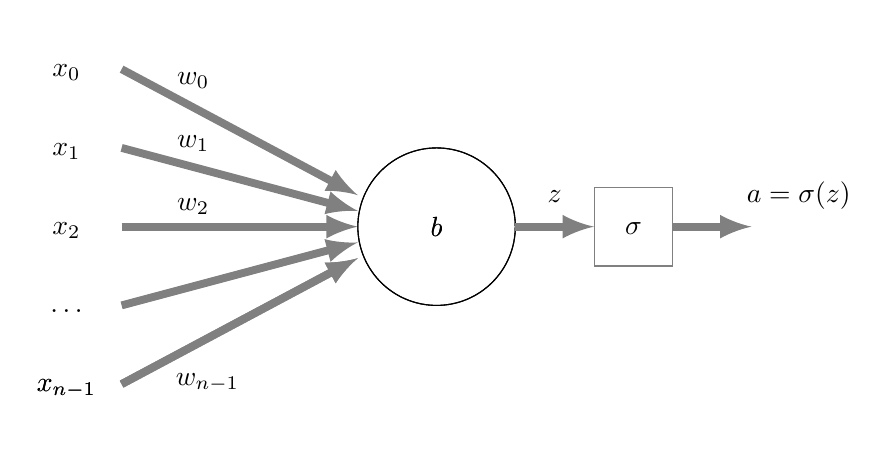
\begin{tikzpicture}[
		axtxt/.style={  
			draw=none,
			text height=1.5ex,
			text depth=.25ex,
			minimum height=3em,
		}]
		\def\L{3.}; \def\dxt{-0.7}; \def\dy{1.}; \def\dyl{0.2};
		
	    \def\n{2};
	    	\draw [line width=.1cm, gray,-latex] (0,\dy*\n) -- (\L,\n*\dyl);
	    	\node[axtxt] at (\dxt,\dy*\n) {$x_0$};
	    	\node[axtxt] at (-\dxt*1.3,\dy*\n-0.1) {$w_0$};
	    \def\n{1};
	    	\draw [line width=.1cm, gray,-latex] (0,\dy*\n) -- (\L,\n*\dyl);
	    	\node[axtxt] at (\dxt,\dy*\n) {$x_1$};
	    	\node[axtxt] at (-\dxt*1.3,\dy*\n+0.1) {$w_1$};
	    \def\n{0};
	    	\draw [line width=.1cm, gray,-latex] (0,\dy*\n) -- (\L,\n*\dyl);
	    	\node[axtxt] at (\dxt,\dy*\n) {$x_2$};
	    	\node[axtxt] at (-\dxt*1.3,\dy*\n+0.3) {$w_2$};
	    \def\n{-1};
	    	\draw [line width=.1cm, gray,-latex] (0,\dy*\n) -- (\L,\n*\dyl);
	    	\node[axtxt] at (\dxt,\dy*\n) {$\ldots$};
	    \def\n{-2}; 
	    	\draw [line width=.1cm, gray,-latex] (0,\dy*\n) -- (\L,\n*\dyl);
	    	\node[axtxt] at (\dxt,\dy*\n) {$x_{n-1}$};
	    	\node[axtxt] at (-\dxt*1.3+0.18,\dy*\n+0.08) {$w_{n-1}$};
	    
	    \def\R{1}; 	
	    \draw (\L+\R,0) circle [radius=\R] node {$b$};
	    \draw (\L+\R,0) circle [radius=\R] node {$b$};
	    
	    \draw [line width=.1cm, gray,-latex] (0,\dy*\n) -- (\L,\n*\dyl);
	    \node[axtxt] at (\dxt,\dy*\n) {$x_{n-1}$};
	    
	    \draw [line width=.1cm, gray,-latex] (\L+\R*2,0) -- (\L+\R*2+1.,0);
	    \node[axtxt] at (\L+\R*2+0.5,0.4) {$z$};
	    
	    \def\S{1}; 
	    \filldraw[fill=white, draw=gray] (\L+\R*2+1.,\S*0.5) rectangle (\L+\R*2+\S+1.,-\S*0.5);
	    \node[axtxt] at (\L+\R*2+\S*0.5+1.,0) {$\sigma$};
	    
	   	\draw [line width=.1cm, gray,-latex] (\L+\R*2+\S+1.,0) -- (\L+\R*2+\S+1.+1.,0);
	    \node[axtxt] at (\L+\R*2+\S+1.+1.+0.6,0.4) {$a=\sigma(z)$};
	    
	\end{tikzpicture}
  	\caption{
  		схематическое изображение искусственного нейрона (для наглядности функция активации вынесена отдельно) и используемые в данной работе обозначения.
  		Входной сигнал нейрона, имеющего $n$ входов, обозначается вектором $\vect{x}$ длины $n$ с элементами $x_0, x_1, \ldots, x_{n-1}$.
  		Совокупность весов входов нейрона обозначается как вектор $\vect{w}$ длины $n$ с элементами $w_0, w_1, \ldots, w_{n-1}$, смещение нейрона обозначено символом $b$, взвешенный выход как $z$ ($z=\vect{w}^T \vect{x} + b$), а функция активации как $\sigma$.
  		Результирующий выход нейрона после действия функции активации на взвешенный выход тогда запишется как $a=\sigma(z)$.
  	}
  	\label{fig:neuron}
\end{figure}

На рисунке~\ref{fig:neuron} приводится схематическое изображение одного нейрона ИНС с использованием введенных выше обозначений.
Нейрон имеет $n$ входов, каждый из которых соответствует одной из наблюдаемых переменных (в нашем случае, полученным баллам за один из экзаменов), и каждому входу приписывается соответствующий вес.
Вектор весов нейрона $\vect{w}$, а также смещение $b$ образуют набор параметров нейрона, и задачей обучения сети является фактически выбор их оптимальных значений.
Также нейрон характеризуется используемой функцией активации $\sigma$ (гиперпараметр).

Принцип работы нейрона соответственно можно описать следующим образом.
\begin{enumerate}
	\item На вход нейрона подается вектор наблюдаемых переменных $\vect{x}$ длины $n$.
	\item С использованием текущих значений весов и смещения нейрона (задаваемых вектором $\vect{w}$ длины $n$ и числом $b$), вычисляется взвешенный выход нейрона $z = \vect{w}^T \vect{x} + b$.
	\item Используемая в данном нейроне функция активации $\sigma$ действует на взвешенный выход нейрона, и соответственно получаем окончательный выход нейрона $a = \sigma(z)$ (число, в большинстве реализаций лежащее в отрезке $[0, 1]$), который является предсказанием значения исследуемой величины.
\end{enumerate}

\begin{figure}[t!]
	\center{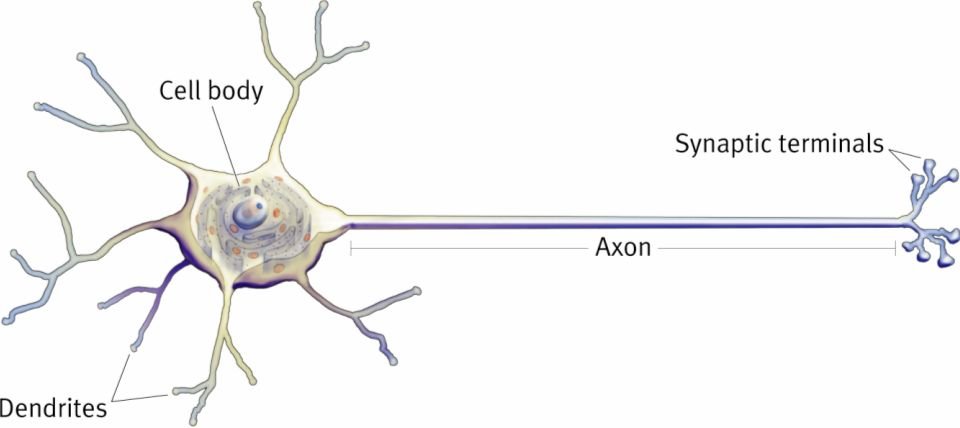
\includegraphics[width=1\linewidth]{../pictures/neuron_real.jpg}}
	\caption{
		Схематическое изображение нейрона головного мозга.
        }
        \label{fig:neuron_real}
\end{figure}

На рисунке~\ref{fig:neuron_real}\footnote{
	Данное изображение заимствовано с веб-ресурса \url{http://bio3520.nicerweb.com/Locked/chap/ch03/neuron.html}.
}
изображены основные элементы реального нейрона головного мозга, ставшего прототипом для модели искусственного нейрона в ИНС.
В сильно упрощенной форме принцип его действия следующий: дендриты (dendrites) передают телу нейрона (cell body) сигналы от соседних нейронов (вектор входных параметров $\vect{x}$ в модели искусственного нейрона) в виде физико-химических импульсов, причем пропускные способности дендритов различаются и могут меняться с течением времени (веса $\vect{w}$ в модели искусственного нейрона).
Если суммарная величина сигнала (взвешенный выход нейрона $z$ в модели искусственного нейрона) превышает некоторое пороговое значение (роль порогового значения в модели искусственного нейрона играет величина $b$, однако для удобства математического представления в формулах выше она была учтена в выражении для взвешенного выхода нейрона, соответственно, в данном случае для продолжения аналогии, в модели искусственного нейрона в качестве порогового значения можно указать нуль), то активизируется выход аксона (axon) нейрона (имеется определенная аналогия с функцией активации $\sigma$ в модели искусственного нейрона), и сигнал передается далее по нейронной сети мозга. При этом, если на некоторый дендрит сигнал от соседних нейронов поступает редко, то происходит снижение его проводящих свойств, а в противном случае -- повышение, что является аналогией для классического алгоритма обучения искусственных нейронов и ИНС, который будет рассмотрен далее в работе. 

\newpage
\subsection{Полносвязные искусственные нейронные сети} \label{ss:review_nn}

В данном разделе мы последовательно сформулируем принцип действия полносвязной ИНС, составленной из искусственных нейронов, которые были описаны в предыдущем разделе.
Приводимые выкладки будут использованы нами далее в работе при программной реализации ИНС данного типа для решения задачи распознавания символов на графических изображениях, а именно для автоматического распознавания CAPTCHA.

На рисунке~\ref{fig:nn}\footnote{
	Данное изображение заимствовано с веб-ресурса \url{https://people.cs.pitt.edu/~xianeizhang/notes/NN/NN.html}.
}
схематически изображена полносвязная нейронная сеть, которая может быть использована для задачи распознавания цифры, представленной на графическом монохромном изображении.
На рисунке~\ref{fig:nn_digits}\footnote{
	Данное изображение заимствовано с веб-ресурса \url{http://neuralnetworksanddeeplearning.com/chap1.html}.
}
в качестве примера приведен набор из рукописных цифр, каждую из которых (после сегментации исходного изображения) можно распознать посредством ИНС.
В рассматриваемом примере монохромное изображение размера $28 \times 28$ пикселей представляется в виде входного вектора (input vector) $\vect{x}$ длины $748$ (для этого необходимо матрицу значений интенсивностей пикселей развернуть в вектор, производя последовательный обход строка за строкой, либо столбец за столбцом), в качестве значений содержащего интенсивности соответствующих пикселей.
Данный вектор подается на входной слой (input layer) ИНС, содержащий аналогичное число ($748$) входных нейронов.
Входной слой по своей сути является формальным -- в нем не выполняется никаких преобразований сигнала, а основное его предназначение -- это ввод сигнала в ИНС и передача его на следующий, внутренний слой (hidden layer) ИНС (то есть фактически входной слой составлен из обычных приемников сигнала, или формально -- из нейронов с единичным весом, нулевым смещением и тождественной функцией активации).

Каждый нейрон внутреннего слоя ИНС устроен в точности так, как было подробно описано в предыдущем разделе и изображено на рисунке~\ref{fig:neuron}.
Соответственно, на внутреннем слое происходит преобразование сигнала каждым нейроном слоя, а полученный промежуточный выходной сигнал передается на выходной слой (output layer), где также происходит дополнительное преобразование сигнала нейронами выходного слоя.
В простейшем случае выходной слой состоит из таких же нейронов, как и внутренний слой, и после преобразования ими сигнала, полученный результирующий сигнал (output vector), собственно и является результатом работы сети.
Для случая распознавания цифр, выходной слой обычно имеет $10$ нейронов, соответственно длина выходного вектора $\vect{y}$ равна $10$, а $k$-ый ($k=0, 1, \ldots, 9$) его элемент соответствует вероятности того, что на входном изображении представлена цифра $k$.
В рассматриваемом случае в качестве итогового ответа сети можно рассматривать $v = argmax (\vect{y})$, т.е. номер элемента выходного вектора, имеющего наибольшее значение.
Этот номер и будет предсказанным (распознанным) сетью числом на изображении.

\begin{figure}[t!]
	\center{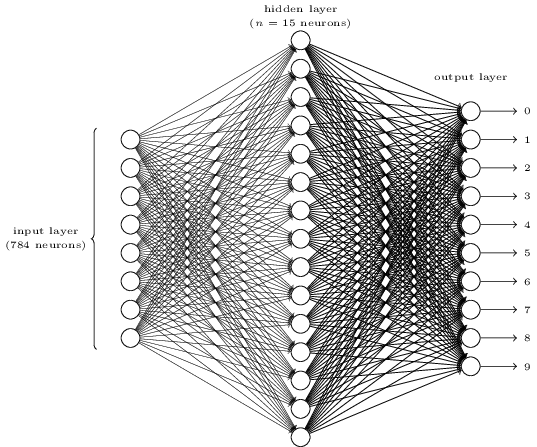
\includegraphics[width=1\linewidth]{../pictures/nn.png}}
	\caption{
		Схематическое изображение полносвязной ИНС.
		Входной вектор $\vect{x}$ сети для данного примера имеет длину $748$ (и соответственно столько же нейронов находится во входном слое ИНС), что соответствует интенсивностям пикселей монохромного изображения размера $28 \times 28$.
		Число нейронов выходного слоя (и соответственно, размерность выходного вектора $\vect{y}$) равно $10$, что соответствует задаче распознавания цифры, представленной на входном изображении.
		Внутренний слой изображенной ИНС состоит из $15$ нейронов (количество нейронов внутреннего слоя -- это один из гиперпараметров сети).
        }
        \label{fig:nn}
\end{figure}

Поскольку в приведенной модели ИНС каждый нейрон внутреннего слоя связан с каждым нейроном входного слоя, а каждый нейрон выходного слоя связан с каждым нейроном промежуточного слоя, то такие сети называют полносвязными ИНС (при наличии нескольких внутренних слоев соответствующие сети обычно называют глубокими или глубинными полносвязными ИНС).
Отметим, что, например, каждый нейрон выходного слоя имеет число входов, равное числу нейронов внутреннего слоя, при этом входным вектором значений для каждого из нейронов выходного слоя является вектор, составленный из выходов всех нейронов внутреннего слоя ($a_0, a_1, \ldots, a_{14}$ для примера ИНС с $15$-ю нейронами во внутреннем слое, изображенной на рисунке~\ref{fig:nn}).

Теперь мы введем систему обозначений, которую будем использовать далее в работе, для рассматриваемой модели полносвязной ИНС.

\begin{itemize}
	\item 
		Пусть $L$ -- это число слоев ИНС\footnote{
			Формально при количестве слоев $L>3$, то есть при наличии более чем одного внутреннего слоя, ИНС является глубокой (deep).
			Однако обычно данный термин применяют для сетей с числом слоев значительно больше $3$-х, например, $10$ слоев.
		}
		(в приведенном выше примере $L=3$).
		При этом, для обозначения конкретного слоя сети будем использовать символ $l$ с нумерацией, начинающейся с нуля (соответственно, $l=0, 1, \ldots, L-1$).
	\item 
		Количество нейронов в $l$-ом ($l=0, 1, \ldots, L-1$) слое  будем обозначать как $N^{(l)}$ (в приведенном выше примере $N^{(0)}=784$, $N^{(1)}=15$, $N^{(2)}=10$).
		При этом, для обозначения конкретного нейрона будем обычно использовать символ $i$ или $j$ с нумерацией, начинающейся с нуля (соответственно, $i=0, 1, \ldots, N^{(l)}-1$ для $l$-ого слоя при $l=0, 1, \ldots, L-1$).
	\item 
		Вектор, подаваемый на вход ИНС (например, вектор, состоящий из определенным образом упорядоченных значений интенсивности пикселей анализируемого изображения) будем обозначать как $\vect{x}$ и называть входом ИНС или входным вектором ИНС (вектором, поданным на вход сети)\footnote{
			Мы не вводим специальных обозначений для входных векторов нейронов внутренних слоев и нейронов выходного слоя, поскольку входными векторами нейронов $l$-ого слоя ($l=1, 2, \ldots, L-1$) являются выходные векторы предыдущего, $(l-1)$-ого слоя.
		}.
		Отметим, что длина вектора $\vect{x}$ и число нейронов входного слоя $N^{(0)}$ должны в точности совпадать.
	\item 
		Смещение $j$-ого нейрона  ($j=0, 1, \ldots, N^{(l)}-1$) $l$-ого слоя  ($l=0, 1, \ldots, L-1$) будем обозначать как $b_j^{(l)}$, а соответствующие упорядоченные значения для всех нейронов $l$-ого слоя объединим в вектор $\vect{b}^{(l)}$ длины $N^{(l)}$.
	\item 
		Для $j$-ого нейрона  ($j=0, 1, \ldots, N^{(l)}-1$) $l$-ого слоя ($l=1, 2, \ldots, L-1$, при этом входной слой не рассматривается) определим $i$-ый вес  или вес его $i$-ого входа как $w_{ji}^{(l)}$ (подчеркнем, что $i$-ый вес является выходом $i$-ого нейрона $(l-1)$-ого слоя, соответственно $i=0, 1, \ldots, N^{(l-1)}-1$).
		Веса всех нейронов $l$-ого слоя сети ($l=1, 2, \ldots, L-1$) для удобства математических выкладок соберем в матрицу $\matr{W}^{(l)}$ размера $N^{(l)} \times N^{(l-1)}$, в которой $\matr{W}^{(l)} [j, i] = w_{ji}^{(l)}$, то есть элемент матрицы на пересечении $j$-ой строки и $i$-ого столбца -- это $i$-ый вес $j$-ого нейрона $l$-ого слоя.
	\item
		Взвешенный выход $j$-ого нейрона  ($j=0, 1, \ldots, N^{(l)}-1$) $l$-ого слоя  ($l=0, 1, \ldots, L-1$) будем обозначать как $z_j^{(l)}$, а соответствующие упорядоченные значения для всех нейронов $l$-ого слоя объединим в вектор $\vect{z}^{(l)}$ длины $N^{(l)}$.
	\item
		Функцию активации нейронов $l$-ого слоя  ($l=0, 1, \ldots, L-1$) будем обозначать как $\sigma^{(l)}$ (все нейроны в одном слое всегда имеют одну и ту же функцию активации), а для случая использования одинаковой функции активации для всех слоев сети будем использовать обозначение $\sigma$, то есть опускать индекс, соответствующий номеру слоя.
	\item
		Выход $j$-ого нейрона  ($j=0, 1, \ldots, N^{(l)}-1$) $l$-ого слоя  ($l=0, 1, \ldots, L-1$) будем обозначать как $a_j^{(l)}$, а соответствующие упорядоченные значения для всех нейронов $l$-ого слоя объединим в вектор $\vect{a}^{(l)}$ длины $N^{(l)}$.	
		Выход последнего слоя (выходного слоя) $\vect{a}^{(L-1)}$ является результатом работы (предсказанием) ИНС и называется выходом ИНС или выходным вектором ИНС.
	\item
		В случае, если для данного входа ИНС (вектора $\vect{x}$) известно правильное значение моделируемого свойства (например, цифра, представленная на изображении), то выход сети, соответствующий этому правильному значению, будем обозначать $\vect{y}$ и называть желаемым выходом сети \footnote{
		Например, если известно, что на изображении представлен нуль, то желаемым выходом ИНС с десятью нейронами в выходном слое будет вектор длины $10$, в котором первый элемент равен единице, а остальные являются нулями. Очевидно, данный вектор будет соответствовать предсказанию сети, отвечающему стопроцентной вероятности того, что на изображении представлен нуль.
		}.
	\item
		Функцию $C_{\vect{x}}$, зависящую от выхода ИНС $\vect{a}^{(L-1)}$ (а значит от архитектуры сети, в частности, от значений весов и смещений всех нейронов сети) и желаемого выхода ИНС $\vect{y}$ для данного значения входа ИНС $\vect{x}$ будем называть функцией стоимости отдельного измерения.
	\item
		Если имеется обучающая выборка размера $M$, то есть, $M$ пар входных векторов $\vect{x}_q$ и соответствующих желаемых выходов $\vect{y}_q$ ($q=0, 1, \ldots, M-1$), то функцией стоимости будем называть функцию вида
		$$
			C = \frac{1}{M} \sum_{q=0}^{M-1} C_{\vect{x}_q},
		$$
		где $C_{\vect{x}_q}$ -- это функция стоимости отдельного измерения, соответствующего $q$-ому элементу выборки.
\end{itemize}

\begin{figure}[t!]
	\center{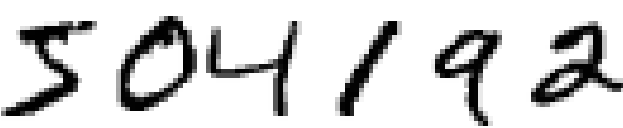
\includegraphics[width=1\linewidth]{../pictures/nn_digits.png}}
	\caption{
		Пример изображения с рукописными цифрами, каждая из которых после сегментации исходного изображения на отдельные символы может быть распознана посредством ИНС.
        }
        \label{fig:nn_digits}
\end{figure}

Отметим, что смещения и функция активации для нейронов входного слоя ввиду формальной его структуры не имеют прямого смысла, однако для удобства будем полагать, что вектор смещений нейронов входного слоя -- это нулевой вектор, а функция активации -- это тождественная функция.
Взвешенный выход и (итоговый) выход входного слоя соответственно совпадают со входным вектором сети.
При этом, очевидно, что введенная выше матрица весов явно учитывает формальный характер входного слоя ИНС.

Учитывая модель искусственного нейрона, представленную в предыдущем разделе, можем записать для взвешенного выхода $j$-ого нейрона $l$-ого слоя
\begin{equation} \label{ss:review_nn_def_z_part}
	z_j^{(l)} = \sum_{i=0}^{N^{(l-1)}-1} w_{ji}^{(l)} a_i^{(l-1)} + b_j^{(l)}, \quad
	j = 0, 1, \ldots, N^{(l)}-1, \quad
	l = 1, 2, \ldots, L-1,
\end{equation}
а для взвешенного выхода первого слоя ($l=0$) с учетом его формального характера
\begin{equation} \label{ss:review_nn_def_z_part_l0}
	z_j^{(0)} = x_j, \quad
	j = 0, 1, \ldots, N^{(0)}-1.
\end{equation}
Отметим, что в формуле~\eqref{ss:review_nn_def_z_part} учтено, что $i$-ый вход любого нейрона $l$-ого слоя является выходом $i$-ого нейрона  $(l-1)$-ого слоя.

Формулы~\eqref{ss:review_nn_def_z_part} и~\eqref{ss:review_nn_def_z_part_l0} могут быть переписаны более компактно в векторном виде
\begin{equation} \label{ss:review_nn_def_z}
	\vect{z}^{(0)} = \vect{x}, \quad
	\vect{z}^{(l)} = \matr{W}^{(l)} \vect{a}^{(l-1)} + \vect{b}^{(l)}, \quad
	l = 1, 2, \ldots, L-1,
\end{equation}
где использована матрица весов $l$-ого слоя, введенная выше, и соответствующее суммирование заменено на эквивалентную операцию матрично-векторного произведения.

Выход (итоговый) нейронов $l$-ого слоя можем получить, подействовав функцией активации на соответствующий взвешенный выход.
В векторной форме можем записать\footnote{
	В данной формуле функция активации действует на вектор, соответственно результат является также вектором, каждый элемент которого -- это результат действия функции активации на соответствующий элемент векторного аргумента.
}
\begin{equation} \label{ss:review_nn_def_a}
	\vect{a}^{(0)} = \vect{x}, \quad
	\vect{a}^{(l)} = \sigma^{(l)} (\vect{z}^{(l)}) = \sigma^{(l)} (\matr{W}^{(l)} \vect{a}^{(l-1)} + \vect{b}^{(l)}), \quad
	l = 1, 2, \ldots, L-1.
\end{equation}

Таким образом, математически процесс распространения сигнала в ИНС описывается следующим образом.
\begin{enumerate}
	\item
		На вход сети подается входной вектор $\vect{x}$, имеющий длину, равную числу нейронов первого (входного) слоя.
	\item
		Взвешенный выход и выход (итоговый) входного слоя сети задаются как
		$$
			\vect{z}^{(0)} = \vect{x}, \quad
			\vect{a}^{(0)} = \vect{x}.
		$$
	\item
		Для каждого из последующих слоев сети (в цикле) вычисляются взвешенный выход и выход (итоговый) на основе выхода предыдущего слоя
		$$
			\vect{z}^{(l)} = \matr{W}^{(l)} \vect{a}^{(l-1)} + \vect{b}^{(l)}, \quad
			\vect{a}^{(l)} = \sigma^{(l)} (\vect{z}^{(l)}), \quad
			l = 1, 2, \ldots, L-1.
		$$
	\item
		Выход последнего слоя (выходного слоя) $\vect{a}^{(L-1)}$ является результатом работы (предсказанием) ИНС или выходным вектором ИНС.
	\item
		Если для текущего входного вектора $\vect{x}$ известен желаемый выход сети $\vect{y}$ (элемент данных обучающей выборки), то может быть также вычислена функция стоимости отдельного измерения $C_{\vect{x}}$, которая затем используется для обучения (подстройки весов и смещений) ИНС.
\end{enumerate}

Например, для задачи распознавания цифры на изображении, входной вектор $\vect{x}$ -- это интенсивности пикселей изображения, а результат работы сети -- это вектор $\vect{a}^{(L-1)}$, максимальный элемент которого может считаться предсказываемым числом на изображении.
Отметим, что если известно реально представленное на изображении число (то есть, рассматривается элемент обучающей выборки), то составляется соответствующий вектор желаемого выхода $\vect{y}$ длины $10$ с единственным ненулевым (и равным единице) элементом в позиции, соответствующей числу, представленному на изображении.
С использованием выходного вектора ИНС $\vect{a}^{(L-1)}$ и желаемого выходного вектора $\vect{y}$, может быть вычислена функция стоимости (отдельного измерения) $C_{\vect{x}}$ для данного элемента данных, с использованием которой может быть проведено обучение сети, то есть, коррекция значений весов и смещений всех или некоторых нейронов сети.
Одним из популярных выборов функции стоимости является, например, квадратичная функция вида
\begin{equation} \label{ss:review_nn_def_C_quad}
	C_{\vect{x}} = 
		\frac{1}{2} || \vect{y} - \vect{a}^{(L-1)} ||^2 =
		\frac{1}{2} \sum_{j=0}^{N^{(L-1)}-1} \left( \vect{y}[j] - \vect{a}^{(L-1)}[j] \right)^2.
\end{equation}

\newpage
\subsection{Обучение искусственных нейронных сетей} \label{ss:review_nnlearning}

Описанный в предыдущем разделе процесс распространения сигнала в полносвязной ИНС позволяет получить предсказание сети для данного входного вектора и заданных параметров и гиперпараметров сети.
Параметрами сети являются веса и смещения каждого из ее нейронов.
Соответственно, гиперпараметры -- это количество слоев сети, число нейронов в каждом из слоев, вид функции активации для каждого из слоев, вид функции стоимости, а также вводимые далее в данном разделе параметр скорости обучения,  размер подвыборки для обучения методом стохастического градиентного спуска и количество эпох обучения.

При создании ИНС ее параметры инициализируются случайными значениями (с использованием определенных эвристик выбора параметров соответствующих случайных распределений), и предсказание такой (необученной) сети не будет соответствовать правильным (желаемым) значениям.
Таким образом, основной задачей является обучение ИНС, то есть выбор по определенной процедуре таких значений ее параметров (а также, в идеале, и гиперпараметров), что предсказания сети с большой вероятностью являются верными.

Как уже указывалось ранее в работе, для обучения сети необходим набор размеченных данных, то есть $M$-пар вида входной вектор / желаемый выходной вектор (при распознавании цифр на изображении каждый входной вектор -- это упорядоченные интенсивности пикселей изображения, а соответствующий выходной вектор -- это вектор длины $10$, все элементы которого нулевые, кроме элемента, номер которого совпадает с представленной на изображении цифрой).
Набор размеченных данных обычно разбивается на три части:  обучающий набор данных (training data) с числом элементов $M^{(trn)}$, валидационный набор данных (validation data) с числом элементов $M^{(vld)}$ и тестовый набор данных (test data) с числом элементов $M^{(tst)}$.
При этом, очевидно, выполняется
$$
	M^{(trn)} + M^{(vld)} + M^{(tst)} = M.
$$

В простейшем случае, для каждого элемента обучающего набора данных, то есть пары 
$$
	\left( \vect{x}_q, y_q \right), \quad q=0, 1, \ldots, M^{(trn)}-1,
$$
где $\vect{x}_q$ -- это входной вектор и $y_q$ -- это желаемый выход ИНС, вычисляется выход ИНС $\vect{a}^{(L-1)}$, а затем функция стоимости отдельного измерения $C_{\vect{x}_q}$, которая, очевидно, зависит от текущих значений весов и смещений нейронов сети.

Вычислив соответствующие функции стоимости отдельных измерений для всех элементов обучающего набора, можно построить итоговую функцию стоимости
\begin{equation} \label{ss:review_nnlearning_C}
	C = \frac{1}{M^{(trn)}} \sum_{q=0}^{M^{(trn)}-1} C_{\vect{x}_q},
\end{equation}
величина которой пропорциональна ошибке сети.
Процесс обучения (настройки параметров сети) соответственно заключается в выборе таких значений весов и смещений нейронов ИНС, при которых функция стоимости~\eqref{ss:review_nnlearning_C} достигнет минимума.
То есть, фактически функция стоимости из формулы~\eqref{ss:review_nnlearning_C} должа быть рассмотрена как функция весов и смещений всех нейронов сети, и для такой функции многомерного аргумента должен быть найден локальный или глобальный минимум.
Соответствующие значения весов и смещений, обеспечивающие этот минимум, и будут оптимальными значениями параметров сети, при которых она дает максимальную точность.

Явная минимизация функции стоимости является для большинства практически значимых случаев невозможной, поэтому обычно используют итерационный метод градиентного спуска (gradient descent)~\cite{fletcher1963rapidly}.
Данный метод применим для функций многих аргументов.
Для пояснения сути метода, рассмотрим некоторую скалярную функцию $f = f(\vect{x})$ от $N$-мерного (векторного) аргумента $\vect{x} = [x_0, x_1, \ldots, x_{N-1}]^T$.
Запишем приращение функции в некоторой многомерной точке $\vect{x}$ (формулу Тейлора) с точностью первого порядка
\begin{equation} \label{ss:review_nnlearning_graddesc_pre}
	f(\vect{x} + \Delta \vect{x}) \approx
		f(\vect{x}) + \frac{\partial f}{\partial x_0} \Delta x_0 + 
		\frac{\partial f}{\partial x_1} \Delta x_1 + 
		\ldots + 
		\frac{\partial f}{\partial x_{N-1}} \Delta x_{N-1},
\end{equation}
где $\Delta \vect{x} = (x_0, x_1, \ldots, x_{N-1})^T$ -- это малое приращение многомерного аргумента.
Вводя вектор градиента функции
$$
	\vect{\nabla} f = 
		\frac{\partial f}{\partial \vect{x}} =
		\left( \frac{\partial f}{\partial x_0}, \frac{\partial f}{\partial x_1}, \ldots , \frac{\partial f}{\partial x_{N-1}}  \right)^T,
$$
и приращение функции
$$
	\Delta f = f(\vect{x} + \Delta \vect{x}) - f(\vect{x}),
$$
можем переписать формулу~\eqref{ss:review_nnlearning_graddesc_pre} как
\begin{equation} \label{ss:review_nnlearning_graddesc_deltaf}
	\Delta f  \approx ( \vect{\nabla} f )^T \Delta \vect{x}.
\end{equation}
Данная формула отражает практически очевидный факт: приращение функции приблизительно пропорционально приращению аргумента, причем коэффициент пропорциональности -- это градиент функции в соответствующей точке (в случае одномерного аргумента, градиент заменился бы на соответствующую производную).
Отметим, что для корректности формулы~\eqref{ss:review_nnlearning_graddesc_deltaf} необходима непрырывность вторых частных производных функции (только в этом случае правомерно разложение~\eqref{ss:review_nnlearning_graddesc_pre}), а также малость приращения аргумента $\Delta \vect{x}$.

Формула~\eqref{ss:review_nnlearning_graddesc_deltaf} лежит в основе метода градиентного спуска.
Зафиксируем некоторое значение многомерного аргумента функции $\vect{x}$ (например, возьмем некоторое случайное значение из области определения) и вычислим градиент функции в данной точке $\vect{\nabla} f (\vect{x})$.
Дадим теперь приращение аргументу функции в направлении противоположном градиенту
\begin{equation} \label{ss:review_nnlearning_graddesc_deltax}
	\Delta \vect{x} = - \eta \vect{\nabla} f (\vect{x}),
\end{equation}
где положительная величина $\eta$ называется скоростью обучения (learning rate).
Отметим, что величина $\eta$ должна быть достаточно малой для выполнения условия малости приращения аргумента и соответственно применимости разложения~\eqref{ss:review_nnlearning_graddesc_pre}.

Объединяя формулы~\eqref{ss:review_nnlearning_graddesc_deltaf} и~\eqref{ss:review_nnlearning_graddesc_deltax}, получим для приращения функции в точке $\vect{x}$
\begin{equation} \label{ss:review_nnlearning_graddesc_deltaf_fin}
	\Delta f  \approx - \eta ( \vect{\nabla} f )^T \vect{\nabla} f.
\end{equation}

Очивидно, что приращение функции согласно формуле~\eqref{ss:review_nnlearning_graddesc_deltaf_fin} (при выполнении описанных выше условий ее применимости) является отрицательным (или, в редких случаях, нулевым).
Действительно, в правой части данной формулы стоит скалярный квадрат вектора градиента, который является неотрицательным; скорость обучения, которая положительная по определению; соответственно знак <<->> определяет итоговый знак выражения.

Из вышеприведенных соображений напрямую следует компактная формулировка метода градиентного спуска.
Для минимизации функции многих переменных следует взять некоторую случайную точку (значение многомерной переменной), вычислить градиент функции в данной точке и изменить значение аргумента на величину, определяемую формулой~\eqref{ss:review_nnlearning_graddesc_deltax} (то есть, в направлении, противоположном направлению градиента).
Затем для нового значения аргумента следует вновь вычислить градиент и вновь обновить значение аргумента.
Данный шаг повторяется в цикле до выполнения некоторого зафиксированного условия сходимости, например, достаточной малости изменения функции на очередном шаге или достижения максимального числа шагов.
При этом, при выполнении условий на вторые производные функции и на малость скорости обучения, гарантируется, что на каждом шаге значение функции будет становиться все ближе к минимальному, поскольку на каждом шаге значение функции убывает в соответствии с~\eqref{ss:review_nnlearning_graddesc_deltaf_fin}.

Особо подчеркнем, что с одной стороны, чем меньше параметр скорости обучения $\eta$, тем устойчивее и точнее метод градиентного спуска, с другой стороны, чем больше значение данного параметра, тем быстрее работает алгоритм.
Таким образом, при практической реализации ИНС особенно важным является удачный выбор значения параметра скорости обучения (который, фактически является гиперпараметром сети), обеспечивающий одновременно и достаточно точное, и достаточно быстрое обучение сети.
Также отметим, что в нейросетевом подходе каждый шаг обучения (точнее, каждый полный проход обучающего набора данных) называют эпохой (epoch) обучения, при этом для задаваемого числа эпох обучения, которое соответственно также является гиперпараметром сети, будем использовать обозначение $M^{(ep)}$.

Описанный метод градиентного спуска может быть, в принципе, применен для обучения ИНС.
Мы фиксируем некоторые случайные значения весов и смещений нейронов сети.
Для каждого из элементов обучающей выборки мы вычисляем выход сети и соответствующую функцию стоимости отдельного измерения, а затем вычисляем функцию стоимости по формуле~\eqref{ss:review_nnlearning_C}.
Далее находим градиент функции стоимости и изменяем веса и смещения сети на малую величину, в направлении, противоположном градиенту с некоторой скоростью обучения $\eta$.
Для обновленных значений весов и смещений (на очередной эпохе обучения) мы вновь вычисляем функции стоимости отдельных измерений, затем новое значение функции стоимости и ее градиента, и вновь обновляем веса и смещения.
Данный процесс повторяется до тех пор, пока не будут получены веса и смещения сети, при которых функция стоимости достаточно близка к нулю, то есть, пока сеть не научится давать правильные предсказания на обучающем наборе данных или пока не будет достигнуто максимальное число эпох обучения $M^{(ep)}$.

Однако практическая реализация приведенной схемы обучения на основе метода градиентного спуска практически нереальна, поскольку для каждого шага градиентного спуска необходимо заново вычислять выход сети для каждого из элементов обучающего набора, а при крупных обучающих выборках (например, $M^{(trn)} \approx 10^6$), которые применяются в реальных приложениях для обеспечения репрезентативности,  это становится вычислительно сложным.

Используемое на сегодняшний день решение данной проблемы -- это замена классического метода градиентного спуска на его стохастический вариант -- стохастический метод градиентного спуска (stochastic gradient descent)~\cite{bottou2010large}.
Основная идея здесь довольно простая: мы проводим минимизацию функции стоимости согласно описанному выше методу градиентного спуска, однако на каждом его шаге (на каждой эпохе обучения) для построения функции стоимости мы вычисляем функции стоимости отдельных измерений не для всех элементов обучающей выборки, а только для нескольких $M^{(mb)}$ случайно отобранных элементов ($M^{(mb)} << M^{(trn)}$), называемых подвыборкой (mini-batch).
Соответственно, формула~\eqref{ss:review_nnlearning_C} для функции стоимости заменится на
\begin{equation} \label{ss:review_nnlearning_C_stochastic}
	C \approx \frac{1}{M^{(mb)}} \sum_{q=0}^{M^{(mb)}-1} C_{\vect{x}_{r(q)}},
\end{equation}
где $r(q)$ -- это случайное целое неотрицательное число, такое что  $0 \leq r(q) < M^{(trn)}$.
То есть, из всего тестового набора данных размера $M^{(trn)}$ отбирается $M^{(mb)}$ случайных элементов, по которым строится приближение функции стоимости, причем на каждой эпохе обучения отбор случайных элементов производится заново.
В практических приложениях метод стохастического градиентного спуска в большинстве случаев сходится к минимуму, при этом вычислительная сложность относительно обычного градиентного спуска существенно снижается.

Отметим, что крайним случаем метода стохастического градентного спуска является построение подвыборок размера $1$, то есть $M^{(mb)}=1$.
В данном случае на каждой эпохе обучения отбирается только один случайный элемент из обучающего набора данных, и соответственно функция стоимости~\eqref{ss:review_nnlearning_C_stochastic} совпадает с функцией стоимости отдельного измерения.
Вычисленная таким образом функция стоимости используется для обновления весов и смещений нейронов сети.
Поскольку в данном варианте метода фактически не требуется знания всего массива обучающей выборки единовременно (сети просто подается на вход один за другим обучающий примеры, и на каждом примере сеть адаптирует параметры), то такое обучение часто называют обучением на лету.
Например, сети может быть последовательно передано $10$ обучающих примеров, на каждом из которых она <<немного обучится>>, далее сеть используется для работы (предсказаний), а затем, например, сети передается еще один обучающий пример, на котором она еще <<немного обучится>>.
Данный подход является очень привлекательным для практических приложений, однако он не всегда приводит к качественному обучению ИНС.

Последним шагом для реализации практического метода обучения ИНС является построение эффективного метода вычисления градиента функции стоимости для возможности использования стохастического метода градиентного спуска, описанного выше.
Отметим, что существует очевидный метод построения градиента функции на основе конечных разностей.
Так для функции $f = f(\vect{x})$ от $N$-мерного (векторного) аргумента $\vect{x} = [x_0, x_1, \ldots, x_{N-1}]^T$, приводимой выше в качестве примера, градиент в точке $\vect{x}$ может быть вычислен следующим образом.
Мы даем малое приращение $h$ первой координате вектора $\Delta_0 \vect{x} = [x_0+h, x_1, \ldots, x_{N-1}]^T$ и вычисляем
$$
		\frac{\partial f}{\partial x_0} \approx \frac{ f(\vect{x}+ \Delta_0 \vect{x} ) - f(\vect{x})}{h},
$$
затем мы даем приращение только второй координате $\Delta_1 \vect{x} = [x_0, x_1+h, \ldots, x_{N-1}]^T$ и вычисляем
$$
		\frac{\partial f}{\partial x_1} \approx \frac{ f(\vect{x}+ \Delta_1 \vect{x} ) - f(\vect{x})}{h},
$$
и аналогично для остальных координат.
Существенной проблемой данного метода является чрезвычайно высокая вычислительная сложность: для каждого элемента обучающей выборки необходимо произвести вычисления по явным формулам, представленным выше, для каждого веса и каждого смещения для всех нейронов сети.

Данная проблема была решена только в конце 80-х годов прошлого века, когда в работе~\cite{williams1986learning} был предложен (частично переоткрытый) алгоритм обратного распространения ошибки (backpropagation) в ИНС, позволяющий быстро вычислять частные производные функции стоимости по весам и смещениям нейронов сети.

Далее мы сформулируем алгоритм обратного распространения ошибки для полносвязной ИНС, представленной в предыдущем разделе, с использованием соответствующих обозначений, подробно описанных там же.
Отметим, что функция стоимости $C$ на обучающей выборке -- это среднее по выборке от функции стоимости отдельного измерения $C_{\vect{x}_q}$ при $q=0,  1, \ldots, M^{(trn)}-1$ (в соответствии с формулой~\eqref{ss:review_nnlearning_C} или приближенной формулой~\eqref{ss:review_nnlearning_C_stochastic}).
При этом функция стоимости отдельного измерения $C_{\vect{x}_q}$ (определяемая, например, по формуле~\eqref{ss:review_nn_def_C_quad} для случай выбора квадратичной функции стоимости) является мерой отклонения выхода ИНС от желаемого (правильного) значения.
Для заданного элемента обучающей выборки и заданной архитектуры сети $C_{\vect{x}_q}$ зависит только от весов и смещений всех нейронов ИНС, то есть
$$
	C_{\vect{x}_q} = C_{\vect{x}_q} \left(
		\matr{W}^{(1)}, \matr{W}^{(2)}, \ldots, \matr{W}^{(L-1)}, \vect{b}^{(1)}, \vect{b}^{(2)}, \ldots, \vect{b}^{(L-1)}
	\right),
$$
где $\matr{W}^{(l)}$ ($l=1, 2, \ldots L-1$) -- это матрица весов $l$-ого слоя, а $\vect{b}^{(l)}$ ($l=1, 2, \ldots L-1$) -- это вектор смещений $l$-ого слоя (для компактности записи мы объединили веса и смещения нейронов каждого слоя в соответствующие матрицы весов и векторы смещений).
Соответственно для обучения ИНС по методу (стохастического) градиентного спуска нам необходимы выражения для частных производных функции стоимости по всем весам 
$$
	\frac{\partial C_{\vect{x}_q}}{\partial w_{ji}^{(l)}}, \quad
	j = 0, 1, \ldots, N^{(l)}-1, \quad
	i = 0, 1, \ldots, N^{(l-1)}-1, \quad
	l = 1, 2, \ldots, L-1,
$$
и по всем смещениям
$$
	\frac{\partial C_{\vect{x}_q}}{\partial b_{j}^{(l)}}, \quad
	j = 0, 1, \ldots, N^{(l)}-1, \quad
	l = 1, 2, \ldots, L-1,
$$ 
нейронов ИНС (для входного слоя, соответствующего $l=0$, веса отсутствуют, а смещения являются нулевыми).

Дополнительно для удобства выкладок мы введем также формальную величину ошибки нейрона\footnote{
	Производная здесь понимается в смысле производной по сложной функции: функция стоимости зависит от весов и смещений нейронов ИНС, при этом взвешенные выходы нейронов, по которым производится дифференцирование, также зависят от весов и смещений.
}
по формуле
$$
	\delta_j^{(l)} = \frac{\partial C_{\vect{x}}}{\partial z_{j}^{(l)}}, \quad
	j = 0, 1, \ldots, N^{(l)}-1, \quad
	l = 1, 2, \ldots, L-1,
$$
где $C_{\vect{x}}$ -- это функция стоимости ИНС на на конкретном элементе обучающей выборки, а $z_{j}^{(l)}$ -- это взвешенный выход $j$-ого нейрона $l$-ого слоя.
Ошибки нейронов одного слоя можно объединить в соответствующий вектор ошибки нейронов слоя следующим образом
$$
	\vect{\delta^{(l)}} = \frac{\partial C_{\vect{x}}}{\partial \vect{z}^{(l)}}, \quad
	l = 1, 2, \ldots, L-1,
$$
где производная по вектору обозначает вектор, каждая из компонент которого -- это соответствующая частная производная числителя по соответствующей компоненте вектора в знаменателе.

\begin{theorem} \label{th:backprop}
	Для полносвязной искусственной нейронной сети, имеющей $L$ слоев, состоящих из $N^{(0)}, N^{(1)}, \ldots, N^{(L-1)}$ нейронов соответственно, частная производная функции стоимости отдельного измерения $C_{\vect{x}}$ по смещению $j$-ого нейрона ($j = 0, 1, \ldots, N^{(l)}-1$) $l$-ого слоя ($l = 1, 2, \ldots, L-1$) может быть записана как
	\begin{equation} \label{ss:review_nnlearning_C_grad_b}
		\frac{\partial C_{\vect{x}}}{\partial b_j^{(l)}} = \delta_j^{(l)},
	\end{equation}
	а частная производная по $i$-ому весу ($i = 0, 1, \ldots, N^{(l-1)}-1$) $j$-ого нейрона ($j = 0, 1, \ldots, N^{(l)}-1$) $l$-ого слоя ($l = 1, 2, \ldots, L-1$) как
	\begin{equation} \label{ss:review_nnlearning_C_grad_w}
		\frac{\partial C_{\vect{x}}}{\partial w_{ji}^{(l)}} = a_i^{(l-1)} \delta_j^{(l)},
	\end{equation}
	где $\delta_j^{(l)}$ -- это величина ошибки $j$-ого нейрона ($j = 0, 1, \ldots, N^{(l)}-1$) $l$-ого слоя ($l = 1, 2, \ldots, L-1$), которая может быть определена по следующим векторным рекуррентным формулам
	\begin{equation} \label{ss:review_nnlearning_C_grad_delta} 
		\begin{split}	
			\vect{\delta}^{(L-1)} = &
				\frac{\partial C_{\vect{x}}}{\partial \vect{a}^{(L-1)}} \odot \sigma'(\vect{z}^{(L-1)}),
			\\
			\vect{\delta}^{(l)} =  &
				\left( \left( \matr{W}^{(l+1)} \right)^T \vect{\delta}^{(l+1)} \right) \odot \sigma'(\vect{z}^{(l)}),
			\quad
			l = L-2, L-3, \ldots, 1,
		\end{split}
	\end{equation}
	где <<$\odot$>> - это операция поэлементного (Адамарова) перемножения векторов, штрих у функции активации\footnote{
		Для компактности формул мы опускаем номер слоя ($l$) у функции активации.
	} 
	соответствует полной производной по ее аргументу, а остальные величины соответствуют системе обозначений, введенной в разделе~\ref{ss:review_nn}.
\end{theorem}

\begin{proof}
	Докажем истинность первой формулы в~\eqref{ss:review_nnlearning_C_grad_delta}.
	Согласно определению ошибки нейронов, а также правилу дифференцирования сложной функции имеем
	$$
		\delta_j^{(L-1)} = \frac{\partial C_{\vect{x}}}{\partial z_j^{(L-1)}} =
			\sum_{i=0}^{N^{(L-1)}} 
				\frac{\partial C_{\vect{x}}}{\partial a_i^{(L-1)}}
				\frac{\partial a_i^{(L-1)}}{\partial z_j^{(L-1)}},
		\quad
		j = 0, 1, \ldots, N^{(L-1)}-1.
	$$
	Поскольку $a_i^{(L-1)} = \sigma(z_i^{(L-1)})$, то только одно слагаемое в последней формуле отлично от нуля, и
	$$
		\delta_j^{(L-1)} =
			\frac{\partial C_{\vect{x}}}{\partial a_j^{(L-1)}}
			\frac{\partial a_j^{(L-1)}}{\partial z_j^{(L-1)}} =
			\frac{\partial C_{\vect{x}}}{\partial a_j^{(L-1)}}
			\sigma'(z_j^{(L-1)}).
	$$
	Соответственно в векторной форме можем переписать как
	$$
		\vect{\delta}_j^{(L-1)} =
			\frac{\partial C_{\vect{x}}}{\partial \vect{a}^{(L-1)}}
			\sigma'(\vect{z}^{(L-1)}),
	$$
	то есть получаем в точности первую формулу из~\eqref{ss:review_nnlearning_C_grad_delta}.
	
	Теперь докажем рекуррентную формулу (вторую формулу) из~\eqref{ss:review_nnlearning_C_grad_delta}.
	Вновь воспользуемся определением ошибки нейронов и правилом дифференцирования сложной функции с учетом того, что взвешенный выход любого нейрона $(l+1)$-ого слоя определяется (является функцией) взвешенных выходов всех нейронов $l$-ого слоя
	\begin{equation} \label{ss:review_nnlearning_C_grad_delta_tmp}
		\delta_j^{(l)} = \frac{\partial C_{\vect{x}}}{\partial z_j^{(l)}} =
			\sum_{i=0}^{N^{(l+1)}} 
				\frac{\partial C_{\vect{x}}}{\partial z_i^{(l+1)}}
				\frac{\partial z_i^{(l+1)}}{\partial z_j^{(l)}},
		\quad
		j = 0, 1, \ldots, N^{(l)}-1,
		\quad
		l = 1, 2, \ldots, L-2.
	\end{equation}
	Производная от функции стоимости под знаком суммы -- это ошибка соответствующего нейрона $(l+1)$-ого слоя.
	Учитывая также, что по определению взвешенного выхода
	$$
		z_i^{(l+1)} = 
			\sum_{k=0}^{N^{(l)}-1}
				w_{ik}^{(l+1)} a_k^{(l)} + b_i^{(l+1)} =
			\sum_{k=0}^{N^{(l)}-1}
				w_{ik}^{(l+1)} \sigma(z_k^{(l)}) + b_i^{(l+1)},
	$$
	то есть
	$$
		\frac{\partial z_i^{(l+1)}}{\partial z_j^{(l)}} = 
				w_{ij}^{(l+1)} \sigma'(z_j^{(l)}),
	$$
	где штрих у функции активации означает полную производную по аргументу, можем переписать~\eqref{ss:review_nnlearning_C_grad_delta_tmp} в следующей форме
	$$
		\delta_j^{(l)} =
			\sum_{i=0}^{N^{(l+1)}-1} 
				\delta_i^{(l+1)} w_{ij}^{(l+1)} \sigma'(z_j^{(l)}) =
			\left( \sum_{i=0}^{N^{(l+1)}-1}  w_{ij}^{(l+1)} \delta_i^{(l+1)} \right) \sigma'(z_j^{(l)}).
	$$
	Поскольку выражение в скобках -- это соответствующий элемент матрично-векторного произведения для матрицы весов $(l+1)$-ого слоя и вектора ошибок нейронов $(l+1)$-ого слоя, то, в итоге, можем переписать данную формулу в векторной форме как
	$$
		\vect{\delta}^{(l)} = \left( \left( \matr{W}^{(l+1)} \right)^T \vect{\delta}^{(l+1)} \right) \odot \sigma'(\vect{z}^{(l)}),
	$$
	что в точности соответствует второй формуле из~\eqref{ss:review_nnlearning_C_grad_delta}.
	
	Для доказательства формулы~\eqref{ss:review_nnlearning_C_grad_b} перепишем производную по смещению нейрона через производную по соответствующему взвешенному выходу, используя правило дифференцирования сложной функции
	$$
		\frac{\partial C_{\vect{x}}}{\partial b_j^{(l)}} = 
			\frac{\partial C_{\vect{x}}}{\partial z_j^{(l)}}
			\frac{\partial z_j^{(l)}}{\partial b_j^{(l)}},
	$$
	$$
		j = 0, 1, \ldots, N^{(l)}-1,
		\quad
		l = 1, 2, \ldots, L-1,
	$$
	и учитывая определение ошибки нейрона, а также то что по определению
	\begin{equation} \label{ss:review_nnlearning_th_wout_tmp}
		z_i^{(l)} = \sum_{k=0}^{N^{(l)}-1} w_{ik}^{(l)} a_k^{(l-1)} + b_i^{(l)},
	\end{equation}
	получаем
	$$
		\frac{\partial C_{\vect{x}}}{\partial b_j^{(l)}} =  \delta_j^{(l)} \times 1,
	$$
	то есть, искомую формулу~\eqref{ss:review_nnlearning_C_grad_b}.

	И наконец, для доказательства формулы~\eqref{ss:review_nnlearning_C_grad_w} мы, по аналогии, переписываем частную производную по весу нейрона через частную производную по соответствующему взвешенному выходу, используя правило дифференцирования сложной функции
	$$
		\frac{\partial C_{\vect{x}}}{\partial w_{ji}^{(l)}} = 
			\frac{\partial C_{\vect{x}}}{\partial z_j^{(l)}}
			\frac{\partial z_j^{(l)}}{\partial w_{ji}^{(l)}},
	$$
	$$
		j = 0, 1, \ldots, N^{(l)}-1,
		\quad
		i = 0, 1, \ldots, N^{(l-1)}-1,
		\quad
		l = 1, 2, \ldots, L-1,
	$$
	затем, как и выше, мы учитываем определение ошибки нейрона и выражение~\eqref{ss:review_nnlearning_th_wout_tmp}, и, в итоге, получаем
	$$
		\frac{\partial C_{\vect{x}}}{\partial w_{ji}^{(l)}} =  \delta_j^{(l)} a_i^{(l-1)},
	$$
	то есть, формулу~\eqref{ss:review_nnlearning_C_grad_w}.
\end{proof}

Отметим, что при получении предсказания сети (выходного вектора) по заданному входному вектору (алгоритм прямого распространения сигнала по ИНС), как было описано в предыдущем разделе, используется <<прямая>> рекуррентная формула, то есть, последовательно обходятся слои сети, начиная с первого, и выходной вектор одного слоя является входным вектором для следующего слоя.
При этом, согласно приведенной выше теореме, для получения частных производных функции стоимости используется <<обратная>> рекуррентная формула, то есть слои сети обходятся в цикле, начиная с последнего, и для каждого из них вычисляется вектор ошибки нейронов по формуле~\eqref{ss:review_nnlearning_C_grad_delta}.
В этой связи данный алгоритм получил название <<алгоритм обратного распространения ошибки>>.

Доказанная теорема является эффективным инструментом обучения ИНС по заданным обучающим наборам данных в соответствии с методом стохастического градиентного спуска.
С использованием данной теоремы, а также описания процесса распространения сигнала в ИНС, представленного в предыдущем разделе, мы можем теперь схематически описать процесс обучения ИНС, который будет использован нами далее в работе для создания автоматизированной системы распознавания CAPTCHA на основе известных данных по уже распознанным изображениям.

\begin{enumerate}
	\item
		На вход сети подается входной вектор $\vect{x}$, имеющий длину, равную числу нейронов первого (входного) слоя.
		Взвешенный выход и выход (итоговый) входного слоя сети задаются как
		$$
			\vect{z}^{(0)} = \vect{x}, \quad
			\vect{a}^{(0)} = \vect{x}.
		$$
	\item
		Для каждого из последующих слоев сети вычисляем и сохраняем в памяти взвешенный выход и выход по рекуррентным формулам
		$$
			\vect{z}^{(l)} = \matr{W}^{(l)} \vect{a}^{(l-1)} + \vect{b}^{(l)}, \quad
			\vect{a}^{(l)} = \sigma (\vect{z}^{(l)}), \quad
			l = 1, 2, \ldots, L-1.
		$$
		При этом, выход последнего слоя (выходного слоя) $\vect{a}^{(L-1)}$ является результатом работы (предсказанием) ИНС или выходным вектором ИНС.
	\item
		Используя явную форму (производных) функции стоимости отдельного измерения и функции активации, а также значение выходного вектора сети для текущего входного вектора, вычисляем ошибку нейронов последнего слоя по формуле
		$$
			\vect{\delta}^{(L-1)} = \frac{\partial C_{\vect{x}}}{\partial \vect{a}^{(L-1)}} \odot \sigma'(\vect{z}^{(L-1)}).
		$$	
	\item
		Обходим слои в обратном направлении и вычисляем по рекуррентным формулам ошибку нейронов соответствующего слоя, используя явный вид функции активации
		$$
			\vect{\delta}^{(l)} = 
				\left( 
					\left( \matr{W}^{(l+1)} \right)^T \vect{\delta}^{(l+1)} 
				\right) 
				\odot \sigma'(\vect{z}^{(l)}),
			\quad
			l = L-2, L-3, \ldots, 1.
		$$
	\item
		Вычисляем частные производные функции стоимости отдельного измерения по весам и смещениям всех нейронов сети в соответствии с методом обратного распространения ошибок
		\begin{equation} \notag
			\begin{split}
				\frac{\partial C_{\vect{x}}}{\partial b_j^{(l)}} = & \delta_j^{(l)},
				\\
				\frac{\partial C_{\vect{x}}}{\partial w_{ji}^{(l)}} = & a_i^{(l-1)} \delta_j^{(l)},
			\end{split}
		\end{equation}
		для всех $j = 0, 1, \ldots, N^{(l)}-1$, $i = 0, 1, \ldots, N^{(l-1)}-1$, $l = 1, 2, \ldots, L-1$.
	\item
		В соответствии с методом стохастического градиентного спуска, повторяем шаги 1-5 $M^{(mb)}$ раз (собирая подвыборку), сохраняя значения частных производных функции стоимости отдельного измерения по весам и смещениям всех нейронов сети для каждого из измерений, и вычисляем приближенное значение (итоговой) функции стоимости
		$$
			C \approx \frac{1}{M^{(mb)}} \sum_{q=0}^{M^{(mb)}-1} C_{\vect{x}_{r(q)}},
		$$
		а также ее частных производных по весам и смещениям всех нейронов сети ($j = 0, 1, \ldots, N^{(l)}$, $i = 0, 1, \ldots, N^{(l-1)}$ и $l = 1, 2, \ldots, L-1$)
		\begin{equation} \notag
			\begin{split}
				\frac{\partial C}{\partial b_j^{(l)}} \approx &
					\frac{1}{M^{(mb)}} \sum_{q=0}^{M^{(mb)}-1} \frac{\partial C_{\vect{x}_{r(q)}}}{\partial b_j^{(l)}},
				\\
				\frac{\partial C}{\partial w_{ji}^{(l)}} \approx & 
					\frac{1}{M^{(mb)}} \sum_{q=0}^{M^{(mb)}-1} \frac{\partial C_{\vect{x}_{r(q)}}}{\partial w_{ji}^{(l)}},
			\end{split}
		\end{equation}
		где $r(q)$ ($0 \leq r(q) < M^{(trn)}$) -- это номера случайно отбираемых элементов тестовой выборки, а $\vect{x}_{r(q)}$ -- это соответствующие входные векторы.
	\item
		Обновляем веса и смещения всех нейронов сети в соответствии с методом градиентного спуска
		\begin{equation} \notag
			\begin{split}
				b_j^{(l)} \rightarrow & b_j^{(l)} - \eta \frac{\partial C}{\partial b_j^{(l)}},
				\\
				w_{ji}^{(l)} \rightarrow & w_{ji}^{(l)} - \eta \frac{\partial C}{\partial w_{ji}^{(l)}},
			\end{split}
		\end{equation}
		для всех $j = 0, 1, \ldots, N^{(l)}$, $i = 0, 1, \ldots, N^{(l-1)}$ и $l = 1, 2, \ldots, L-1$.
	\item
		Повторяем шаги 1-7 $\frac{M^{(trn)}}{M^{(mb)}}$-раз (полный проход обучающего набора данных).
	\item
		Повторяем шаги 1-8 $M^{(ep)}$-раз, где $M^{(ep)}$ -- это полное число эпох обучения, и сохраняем веса и смещения полученной обученной ИНС.
\end{enumerate}

В заключение раздела отметим, что нами был подробно рассмотрен только один тип ИНС -- полносвязная сеть, наиболее простой в реализации и наименее ресурсоемкий.
В следующем разделе, посвященном анализу методов распознавания CAPTCHA, нами будет также рассмотрен ряд специализированных решений, основанных на подходе ИНС, а в разделе~3 работы мы построим полносвязную ИНС для задачи распознавания CAPTCHA, а также более детально проанализируем наилучший выбор гиперпараметров сети (в частности, функции активации и функции стоимости) и практические аспекты обучения ИНС.
Также стоит отметить, что на сегодняшний день парадигма ИНС остается бурно развивающимся направлением, и регулярно находит новые приложения, в особенности, в области автоматизированной работы с изображениями (распознавание, классификация, сжатие, улучшение, генерация и т.д.).

%=======================================================================
\newpage
\section{Машинное обучение для автоматического распознавания CAPTCHA} \label{s:captheory}

\subsection{Введение} \label{ss:captheory_intro}

Данная глава посвящена анализу методов машинного обучения для распознавания конкретного типа изображений, а именно, основного объекта изучения в данной работе -- CAPTCHA.
Нами будут рассмотрены наиболее распространенные подходы, из числа представленных в научной литературе, для первичной обработки, сегментации CAPTCHA, распознавания отдельных символов, получаемых после сегментации, а также ряд специализированных современных методов для задачи распознавания текстовых изображений и методов для ускорения и снижения потребляемой памяти в задачах распознавания.

В разделе~\ref{ss:captheory_alg} приводится обзор научно-технической литературы, посвященной задаче распознавания CAPTCHA, а также анализируются основные возникающие здесь сложности.
Затем в разделе~\ref{ss:captheory_symb} рассматриваются современные подходы распознавания символьных изображений (буква алфавита или цифра), в частности мы описываем методы прореживания пикселей (thinning) и скелетирования (skeletization) фигур, а также возможные методы выделения важных признаков (features) у символов.
Также в разделе рассматривается процесс первичной подготовки CAPTCHA (удаление лишних цветов, искажений текста, нетекстовой информации и др.) и описываются возможные подходы к задаче сегментации CAPTCHA, то есть разделения текста, представленного на изображении, на отдельные символы.

И наконец, в разделе~\ref{ss:captheory_methods} описываются наиболее современные методы  распознавания текстовой информации на графических изображениях и, в частности, задачи распознавания CAPTCHA.
Нами рассматриваются сверточные искусственные нейронные сети и глубокие искусственные нейронные сети, а также в данном разделе рассматривается наиболее современный, на наш взгляд, подход, получивший свое развитие в последние 2-3 года -- так называемый метод тензоризации глубоких искусственных нейронных сетей.
В основе данного подхода лежит идея представления параметров искусственной нейронной сети в малопараметрических форматах и соответствующая адаптация алгоритмов прямого и обратного распространения сигнала в сети для значительного снижения потребляемой сетью памяти, а также ускорения обучения и функционирования сети.

\newpage
\subsection{Методы распознавания CAPTCHA} \label{ss:captheory_alg}

На сегодняшний день существует большое число научных работ, посвященных теме автоматического распознавания текстовой информации на изображениях CAPTCHA.
Данные исследования имеют следующие цели:
\begin{itemize}
	\item развитие существующих и создание новых методов машинного обучения и интеллектуального анализа данных на примере конкретной (сложной) задачи распознавания CAPTCHA;
	\item выявление общих закономерностей в задачах распознавания текстовой информации на графических изображениях на примере задачи распознавания CAPTCHA для последующего их применения в других приложениях (распознавание текстов, автомобильных и дорожных знаков и т.д.);
	\item создание автоматических систем <<взлома>> конкретных типов CAPTCHA для выявления слабых мест и выработки рекомендаций по улучшению алгоритмов формирования CAPTCHA.
\end{itemize}

В литературе наиболее распространены три условных подхода к задаче распознавания CAPTCHA.
В рамках первого подхода строится некоторый сложный классификатор практически без учета специфики задачи (в большинстве случаев -- это нейросетевой классификатор), который обучается на крупной выборке предварительно распознанных вручную CAPTCHA.
Второй подход предполагает выявление конкретных характерных признаков (feature extraction) или эвристик, позволяющих распознать конкретную CAPTCHA с использованием простейшего классификатора (например, по методу ближайших соседей).
Третий подход комбинирует первый два: предварительно выявленные характерные признаки используются как входной вектор для обучения нейросетевого классификатора.

Отметим, что при практической реализации любого из подходов отдельную сложность представляет предварительная очистка изображения от шумов и помех, а также сегментация, то есть разделение текста, представленного на изображении, на отдельные символы.
Также в ряде работ осуществляется дополнительный анализ результата распознавания, например, если заранее известно, что на CAPTCHA представлено слово из определенного словаря: в этом случае могут быть проверены несколько наиболее вероятных предсказаний классификатора и выбрано то из них, которое содержится в словаре. 
Таким образом, процесс распознавания CAPTCHA можно упрощенно разделить на следующие этапы:
\begin{enumerate}
	\item предварительная обработка изображения, включая удаление шумовых (<<мусорных>>) линий и групп пикселей, бинаризацию изображения, а также в ряде случаев скелетирование (утоньшение) линий;
	\item сегментация изображения на отдельные символы с использованием определенных эвристик или вспомогательного классификатора;
	\item выявление характерных признаков и эвристик, облегчающих процесс распознавания отдельных символов (в качестве характерных признаков могут выступать количество внутренних областей у символа, число самопересечений и т.д.);
	\item формирование обучающей размеченной выборки изображений и обучение классификатора на данной выборке;
	\item пост-анализ результата работы классификатора, включая проверку по корректности длины итогового распознанного символа и принадлежность распознанного текста к определенной словарной базе.
\end{enumerate}

\begin{figure}[t!]
	\center{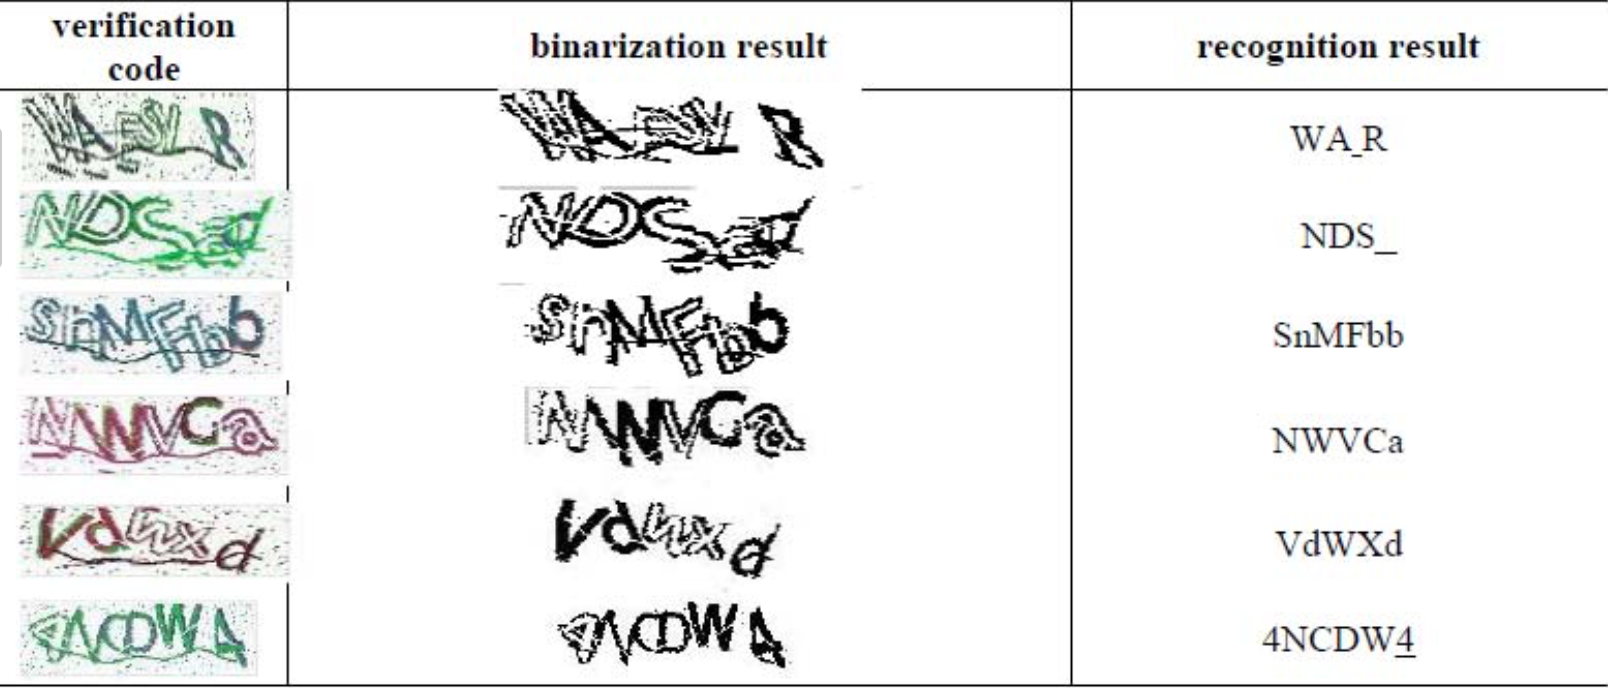
\includegraphics[width=1\linewidth]{../pictures/rev1.png}}
	\caption{
		Пример автоматически распознанных CAPTCHA из работы~\cite{an2017captcha}.
        }
        \label{fig:rev1}
\end{figure}

В работе 2017 г.~\cite{an2017captcha} для распознавания буквенно-циферных CAPTCHA конкретного типа после бинаризации изображения используется метод выделения особенностей формы для каждой точки изображения (relative shape context and point mode).
На рисунке~\ref{fig:rev1} приводится результат распознавания нескольких CAPTCHA из работы.
Как можно видеть, некоторые изображения распознаются существенно неверно, однако для ряда изображений метод дает корректный результат.

\begin{figure}[t!]
	\center{
\includegraphics[width=1\linewidth]{../pictures/rev2.png}}
	\caption{
		Примеры CAPTCHA, анализируемых в работе~\cite{hussain2016recognition}.
        }
        \label{fig:rev2}
\end{figure}

В работе 2016 г.~\cite{hussain2016recognition} проводится распознавание текстовой CAPTCHA, подобных изображенным на рисунке~\ref{fig:rev2} (tmall, JCAPTCHA, Microsoft CAPTCHA).
Особое внимание в работе уделяется сегментации изображения.
Для корректной сегментации на отдельные символы используется скользящее окно переменной ширины: выделенная область изображения отправляется на анализ нейросетевому классификатору (полносвязная ИНС), который был предварительно обучен на распознавание отдельных символов, затем в качестве места расположения символа выбора то положение окна, при котором классификатор дал наибольшую уверенность.
Отдельные символы сегментированного таким образом изображения затем распознаются тем же нейросетевым классификатором.
Заявленная в работе точность сегментации $58.25\%$, а точность распознавания отдельных символов $95\%$.

\begin{figure}[t!]
	\center{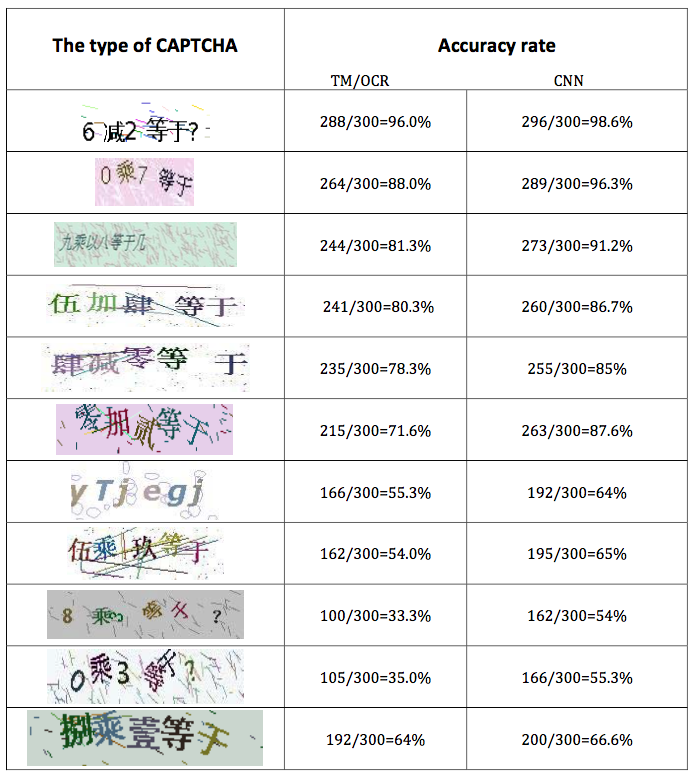
\includegraphics[width=1\linewidth]{../pictures/rev3.png}}
	\caption{
		Результаты распознавания различных CAPTCHA из работы~\cite{wang2017combining}.
        }
        \label{fig:rev3}
\end{figure}

В работе 2017 г.~\cite{wang2017combining} для распознавания нескольких типов CAPTCHA, содержащих цифры и арабские символы, используется сверточная нейронная сеть.
Для сегментации изображения на отдельные символы в работе предлагается использование простейшего метода анализа гистограммы распределения пикселей изображения по горизонтали: в местах, где значение оказывается меньше порогового предполагается окончание очередного символа.
Результаты распознавания приведены на рисунке~\ref{fig:rev3}.
Как можно видеть для ряда классов CAPTCHA точность автоматического распознавания является очень высокой.

\begin{figure}[t!]
	\center{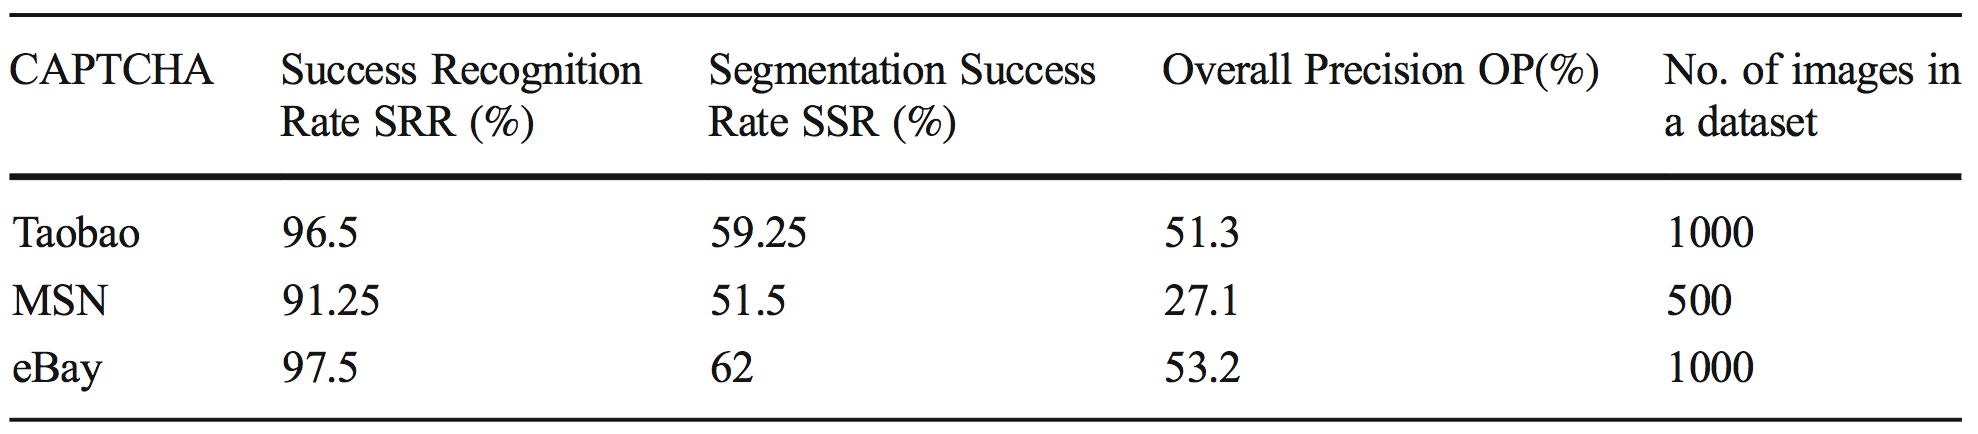
\includegraphics[width=1\linewidth]{../pictures/rev4.png}}
	\caption{
		Результаты распознавания различных CAPTCHA из работы~\cite{hussain2016segmentation}.
        }
        \label{fig:rev4}
\end{figure}

В работе 2016 г.~\cite{hussain2016segmentation} рассматривается задача распознавания буквенно-циферных текстов на CAPTCHA с существенно перекрывающимися символами. На рисунке~\ref{fig:rev4} мы отображаем полученные в работе результаты.

\begin{figure}[t!]
	\center{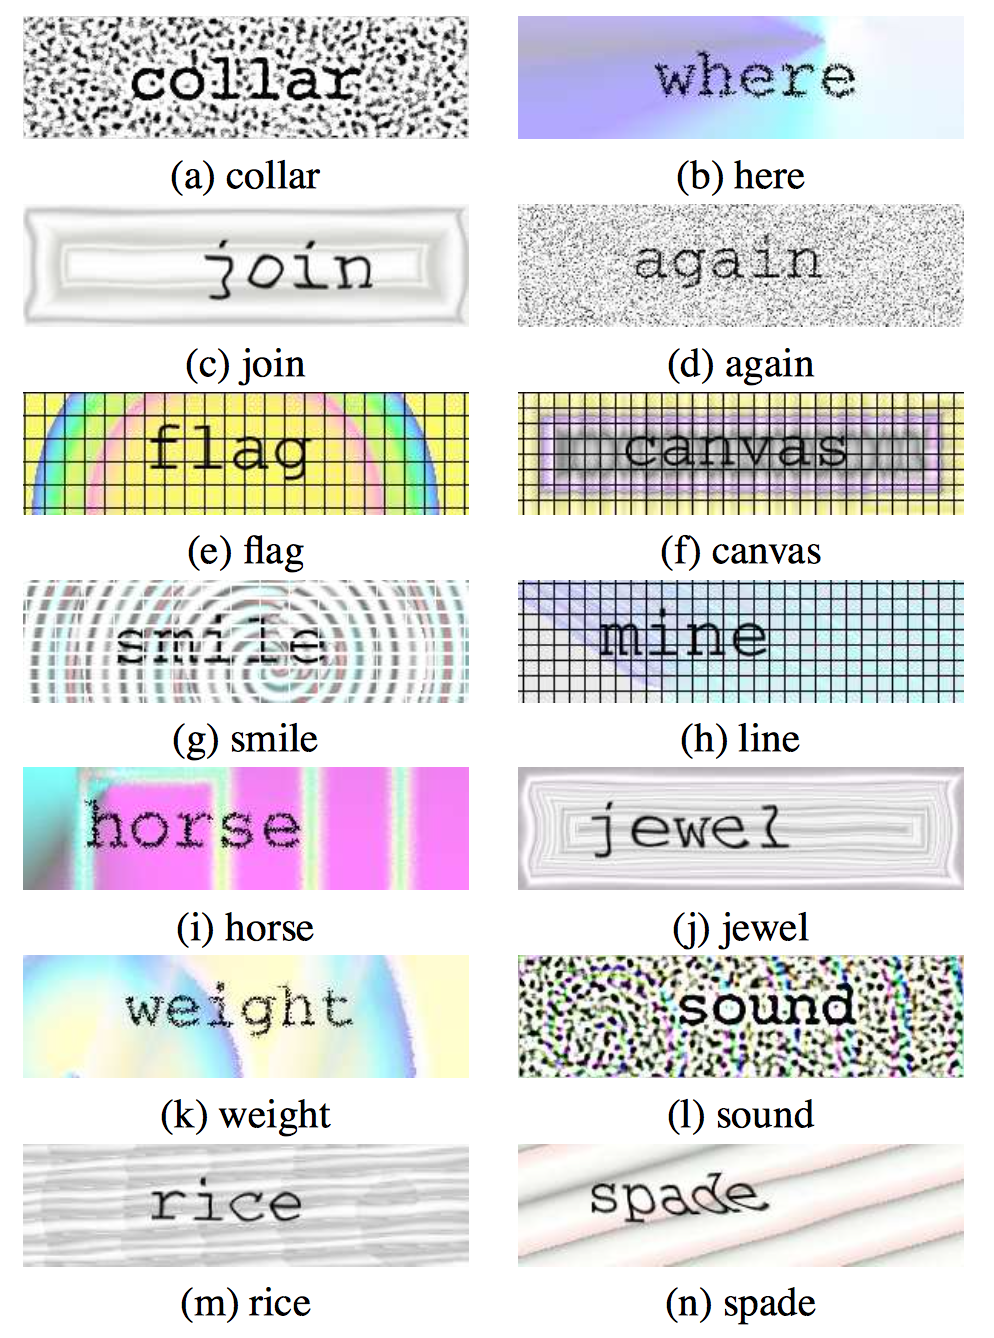
\includegraphics[width=1\linewidth]{../pictures/rev5.png}}
	\caption{
		Результаты распознавания различных CAPTCHA из работы~\cite{mori2003recognizing}.
        }
        \label{fig:rev5}
\end{figure}

Отметим также очень активно цитируемую работу 2003 г.~\cite{mori2003recognizing}, в которой для сегментации и распознавания текстовых CAPTCHA, составленных из слов английского алфавита (см, рисунок~\ref{fig:rev5}) используется набор элегантных методов, основанных на ряде эвристик.
В частности, в данной работе был разработан мощный фреймворк для выделения отдельных символов на основе анализа информации о формах и взаиных расположений закрашенных пикселей бинаризованного изображения.

Таким образом, резюмируя, можно видеть, что направление автоматического распознавания (<<взлома>>) CAPTCHA является активно развивающимся, однако предлагаемые в научных публикациях алгоритмы являются узко направленными и способными относительно эффективно работать только на конкретных классах CAPTCHA.

\newpage
\subsection{Распознавание отдельных символов и сегментация CAPTCHA} \label{ss:captheory_symb}

Программное распознавание символов является сложной задачей машинного обучения, в частности, из-за огромного числа вариантов начертания каждого конкретного символа.
Простейшим (наивным) подходом распознавания символов является простое угадывание, при этом, как ни странно, данный метод имеет определенную точность, например для распознавания цифр точность на достаточно большой и равномерной тестовой выборке составит $10\%$, что может оказаться удовлетворительным для определенных задач.
Еще один наивный подход -- это вычисление суммарной интенсивности пикселей изображений обучающей выборки и последующее сравнение данной величины для тестовых данных с соответствующими шаблонами.
В ряде случаев такой подход может давать достаточно высокую точность, очень сильно зависящую от единообразия начертания символов.

В основе современных подходов распознавания символов лежит идея выделения важных признаков (features; feature extraction) каждого из возможных символов, и последующего обучения классификатора на соответствующей обучающей выборке.
На сегодняшний день существует множество алгоритмов выделения важных признаков у символов и масса моделей классификации, включая методы k-ближайших соседей, главных компонент, радиальных базисных функций, полносвязных и сверточных ИНС (в том числе, глубоких).

В качестве примера мы рассмотрим задачу классификации цифр.
На рисунке~\ref{fig:nn_digits_many}\footnote{
	Данное изображение заимствовано с веб-ресурса \url{http://neuralnetworksanddeeplearning.com/chap1.html}.
}
приводится несколько изображений из базы MNIST~\cite{lecun1998mnist}, содержащей $70000$ распознанных рукописных цифр (от нуля до девяти включительно), написанных различными людьми, в формате изображений размера $28 \times 28$ в градациях серого цвета.
Обычно данный набор разбивается на три части: обучающий набор ($50000$ изображений), валидационный набор ($10000$ изображений) и тестовый набор ($10000$ изображений).
Соответственно, обучающий набор используется для настройки параметров модели (классификатора), на валидационном наборе уточняется выбор гиперпараметров модели, а тестовый набор используется для проверки качества обученной модели.

Простейшим вариантом выделения важных признаков является использование исходных интенсивностей всех пикселей изображения, соответственно, в данном случае мы имеем $784$ ($28 \times 28$) признака для каждого изображения.
В качестве классификатора может быть использована полносвязная ИНС, подробно рассмотренная нами в предыдущем разделе работы, при этом точность классификации цифр может достигать более $96\%$ (см. например~\cite{singh2011digit}).
В такой ИНС входной слой будет иметь $784$ нейрона, а выходной слой -- $10$ нейронов, а результатом распознавания будет считаться номер выхода ИНС (или, эквивалентно, номер элемента выходного вектора ИНС), дающего наибольший сигнал.
Описанный подход является наиболее простым в практическом реализации, так как он не предполагает никакой предварительной обработки изображений, однако при этом существенным является как время обучения/работы модели, так и возможная ошибка результатов.

\begin{figure}[t!]
	\center{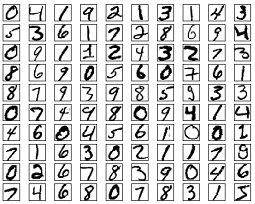
\includegraphics[width=1\linewidth]{../pictures/nn_digits_many.png}}
	\caption{
		Пример рукописных цифр, которые могут быть распознаны посредством ИНС.
        }
        \label{fig:nn_digits_many}
\end{figure}

Более перспективным представляется подход, при котором производится предварительное выделение важных признаков из изображения по определенным алгоритмам, при этом число итоговых признаков может быть существенно меньше, чем количество пикселей в исходном изображений.
Классическим подходом здесь является метод главных компонент~\cite{karamizadeh2013overview}, основанный на сингулярном разложении матрицы признаков.
Элементы обучающего набора данных в данном методе группируются в матрицу (в рассматриваемом примере размера $50000 \times 784$), для которой вычисляется усеченное сингулярное разложение.
Параметр обрезания сингулярного разложения соответственно становится параметром, определяющим степень сжатия исходных признаков, а данный подход позволяет выделять важные признаки без учета детальной структуры изображения.

Большую эффективность однако могут иметь методы, основанные на <<ручном>> выделении существенных признаков.
Так например, рассматривая изображения, представленные на рисунке~\ref{fig:nn_digits_many}, можно увидеть, что характерным признаком нуля является отсутствие концевых пикселей (пикселей, соответствующих концу линии), в то время как для цифр $3$ и $4$ есть три таких пикселя на изображении.
Или, например, для цифры $8$ (и иногда для цифры $2$) имеется пиксель, соответствующий пересечению двух линий.
Другими важными признаками могут быть также наличие и количество углов, внутренних областей (областей фона, окруженных цветными пикселями, как, например, в цифрах нуль и восемь) и т.д.
Подобные эвристики могут быть использованы в эффективном алгоритме выделения существенных признаков, которые затем будут использованы для обучения классификатора.
При этом правила положенные в основу действия классификатора, могут быть как явными, например, для модели решающих деревьев (упрощенный пример здесь может быть таким: <<если на изображении отсутствуют концевые пиксели, а также есть область фона, ограниченная цветными пикселями, значит на изображении представлена цифра $0$>>), так и неявными, например, для модели ИНС, где в процессе последовательного <<изучения>> экземпляров обучающей выборки сеть самостоятельно формулирует решающие правила, представленные в форме весов и смещений сети.
Отметим, что как уже отмечалось ранее в работе, принципиальной слабой стороной нейросетевого подхода является отсутствие возможности увидеть конкретные правила, которыми руководствуется ИНС при принятии решения.
Однако на сегодняшний день уже появился ряд работ, посвященных визуализации структуры ИНС (см., например~\cite{nnvis}).

Описанный выше метод <<ручного>> выделения существенных признаков, тем не менее, не может быть напрямую применен к изображениям, в частности, ввиду их зашумленности.
Так, например, на рисунке~\ref{fig:nn_digits_many} у некоторых изображений присутствуют паразитные (мусорные) пиксели вне изображения, у некоторых четверок есть лишние выступы справа и т.д.
Возможное решение -- это предварительная фильтрация изображения и прореживание пикселей (thinning) или скелетирование (skeletization) форм, представленных на изображении.

Первым шагом в алгоритме фильтрации изображения часто бывает процесс бинаризации, заключающийся в переходе к двухцветовой (бинарной) палитре из нулей и единиц, где нуль соответствует фону, а единица - изображению.
Бинаризация обычно выполняется по некоторому пороговому значению (в предположении, что фон изображения имеет нулевую интенсивность пикселей): если интенсивность некоторого пикселя не превосходит заданное пороговое значение, то такой пиксель удаляется (делается фоновым), при этом простейшим вариантом является использование нулевого порогового значения.
Бинаризованное изображение может быть представлено соответствующей матрицей, состоящей только из нулей и единиц.
Например, для цифры $4$ матрица может иметь вид (для иллюстрации, на изображении представлено также несколько шумовых пикселей)
$$
	\begin{bmatrix}
		0 & 0 & 0 & 0 & 0 & 0 & 0 & 0 \\
		0 & 1 & 0 & 0 & 1 & 1 & 0 & 0 \\
		0 & 1 & 0 & 0 & 1 & 1 & 0 & 0 \\
		0 & 1 & 0 & 0 & 1 & 1 & 0 & 0 \\
		0 & 1 & 1 & 1 & 1 & 1 & 0 & 0 \\
		0 & 0 & 0 & 1 & 1 & 1 & 1 & 0 \\
		0 & 1 & 0 & 0 & 1 & 1 & 1 & 0 \\
		0 & 0 & 0 & 0 & 1 & 1 & 0 & 0	
	\end{bmatrix}
$$

Для очистки бинаризованного изображения от мусорных (шумовых) пикселей может быть использован алгоритм удаления пикселей по девятиточечному шаблону~\cite{babu2014handwritten}.
В данному алгоритме последовательно обходятся все пиксели изображения и соответствующий нефоновый пиксель (равный $1$), удаляется если он соответствует одному из следующих шаблонов (центральный пиксель в представленных шаблонах соответствует текущему анализируемому нефоновому пикселю)
$$
	\begin{bmatrix}
		0 & 0 & 0 \\
		0 & 1 & 0 \\
		0 & 0 & 0
	\end{bmatrix},
	\begin{bmatrix}
		0 & 1 & 0 \\
		0 & 1 & 0 \\
		0 & 0 & 0
	\end{bmatrix},
	\begin{bmatrix}
		0 & 0 & 1 \\
		0 & 1 & 0 \\
		0 & 0 & 0
	\end{bmatrix},
	\begin{bmatrix}
		0 & 0 & 0 \\
		0 & 1 & 1 \\
		0 & 0 & 0
	\end{bmatrix},
	\begin{bmatrix}
		0 & 0 & 0 \\
		0 & 1 & 0 \\
		0 & 0 & 1
	\end{bmatrix},
$$
$$
	\begin{bmatrix}
		0 & 0 & 0 \\
		0 & 1 & 0 \\
		0 & 1 & 0
	\end{bmatrix},
	\begin{bmatrix}
		0 & 0 & 0 \\
		0 & 1 & 0 \\
		1 & 0 & 0
	\end{bmatrix},
	\begin{bmatrix}
		0 & 0 & 0 \\
		1 & 1 & 0 \\
		0 & 0 & 0
	\end{bmatrix},
	\begin{bmatrix}
		1 & 0 & 0 \\
		0 & 1 & 0 \\
		0 & 0 & 0
	\end{bmatrix},
	\begin{bmatrix}
		0 & 0 & 0 \\
		0 & 1 & 1 \\
		0 & 0 & 1
	\end{bmatrix},
$$
$$
	\begin{bmatrix}
		0 & 1 & 0 \\
		0 & 1 & 1 \\
		0 & 0 & 0
	\end{bmatrix},
	\begin{bmatrix}
		1 & 1 & 0 \\
		0 & 1 & 0 \\
		0 & 0 & 0
	\end{bmatrix},
	\begin{bmatrix}
		1 & 0 & 0 \\
		1 & 1 & 0 \\
		0 & 0 & 0
	\end{bmatrix},
	\begin{bmatrix}
		0 & 1 & 0 \\
		1 & 1 & 0 \\
		0 & 0 & 0
	\end{bmatrix},
	\begin{bmatrix}
		0 & 0 & 0 \\
		1 & 1 & 0 \\
		1 & 0 & 0
	\end{bmatrix},
$$
$$
	\begin{bmatrix}
		0 & 0 & 0 \\
		1 & 1 & 0 \\
		0 & 1 & 0
	\end{bmatrix},
	\begin{bmatrix}
		0 & 0 & 0 \\
		0 & 1 & 0 \\
		0 & 1 & 1
	\end{bmatrix},
	\begin{bmatrix}
		1 & 1 & 0 \\
		1 & 1 & 0 \\
		0 & 0 & 0
	\end{bmatrix},
	\begin{bmatrix}
		0 & 1 & 1 \\
		0 & 1 & 1 \\
		0 & 0 & 0
	\end{bmatrix}.
$$
Приведенные шаблоны имеют простой смысл.
Так, например, первый шаблон соответствует ситуации, когда данный пиксель окружен исключительно фоном.
На втором шаблоне отражена ситуация, когда данный пиксель имеет в своем окружении ровно один нефоновый пиксель, который располагается справа от него.
Последний шаблон отвечает случаю, когда данный пиксель имеет ровно три нефоновых пикселя в своем окружении, причем расположены они справа вверху от него.

После проведения бинаризации и очистки изображения от шума, может быть проведена также полезная для последующего выделения ключевых признаков процедура прореживания пикселей.
Суть данного метода заключается в последовательном удалении нефоновых пикселей для преобразования исходного изображения в модифицированное изображение, где все или почти все линии имеет единичную толщину, при сохранении основной информации об изображении.
В обзорных статьях ~\cite{lam1992thinning} и~\cite{gramblivcka2016comparison} рассматриваются основные существующие алгоритмы прореживания.
Мы более подробно остановимся на алгоритме из работы~\cite{zhang1984fast} для последующей реализации данного метода в разрабатываемом нами программном пакете для распознавания CAPTCHA.

\begin{figure}[t!]
	\center{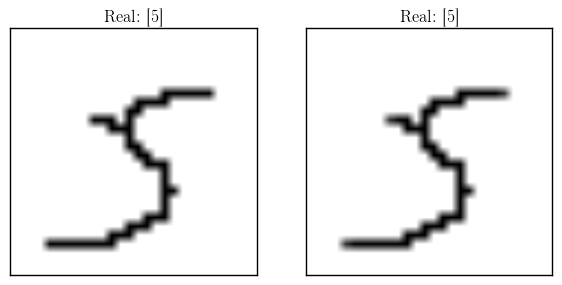
\includegraphics[width=1\linewidth]{../pictures/thin_ex_0.png}}
	\caption{
		Результат прореживания бинаризованного символа $5$ из базы MNIST.
        }
        \label{fig:nn_skelets_ex0}
\end{figure}
  
\begin{figure}[t!]
	\center{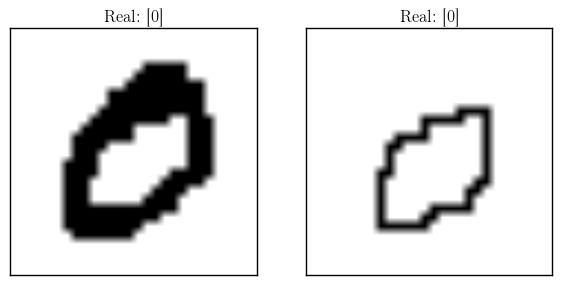
\includegraphics[width=1\linewidth]{../pictures/thin_ex_1.png}}
	\caption{
		Результат прореживания бинаризованного символа $0$ из базы MNIST.
        }
        \label{fig:nn_skelets_ex1}
\end{figure}

В рассматриваемой реализации процедуры прореживания, как и в описанном выше методе фильтрации, используется девятиточечный шаблон для каждого из пикселей изображений.
При этом вводится следующая нумерация пикселей
$$
	\begin{bmatrix}
		P_9 & P_2 & P_3 \\
		P_8 & P_1 & P_4 \\
		P_7 & P_6 & P_5
	\end{bmatrix},
$$
где символ $P_1$ соответствует текущему анализируемому пикселю, а символы $P_2, P_3, \ldots, P_9$ соответствуют его соседям.
Также вводятся две функции: функция $B(P_1)$, равная количеству нефоновых пикселей, соответствующих рассматриваемому пикселю $P_1$
$$
	B(P_1) = P_2 + P_3 + \ldots + P_9,
$$
и функция $A(P_1)$, равная количеству пар вида $0, 1$ в окружении рассматриваемого пикселя.
Так, например, для случая
$$
	\begin{bmatrix}
		0 & 0 & 1 \\
		1 & 1 & 0 \\
		1 & 0 & 0
	\end{bmatrix},
$$
имеем $B(P_1)=3$ и $A(P_1)=2$.

Соответствующий алгоритм прореживания формулируется следующим образом.
Осуществляется двукратный проход всех пикселей изображения, исключая граничные.
Для каждого обнаруженного нефононового пикселя проверяется выполнение четырех условий:
\begin{enumerate}
	\item $2 \leq B(P_1) \leq 6$,
	\item $A(P_1) = 1$,
	\item $P_2 * P_4 * P_6 = 0$,
	\item $P_4 * P_6 * P_8 = 0$,
\end{enumerate}
и в случае выполнения каждого из условий, соответствующий пиксель $P_1$ удаляется (делается фоновым).
На втором проходе проверяется совместное выполнение следующих условий:
\begin{enumerate}
	\item $2 \leq B(P_1) \leq 6$,
	\item $A(P_1) = 1$,
	\item $P_2 * P_4 * P_8 = 0$,
	\item $P_2 * P_6 * P_8 = 0$,
\end{enumerate}
и в случае выполнения каждого из них, соответствующий пиксель $P_1$ удаляется (делается фоновым).
Отметим, что описанный алгоритм на первом проходе удаляет граничные пиксели слева внизу, а на втором проходе -- справа вверху.
Нами был программно реализован данный алгоритм, и на рисунках~\ref{fig:nn_skelets_ex0} и~\ref{fig:nn_skelets_ex1} приводятся результаты прореживания для двух очищенных от шума и бинаризованных изображений из базы MNIST, содержащих цифры $5$ и $0$ соответственно.

\begin{figure}[t!]
	\center{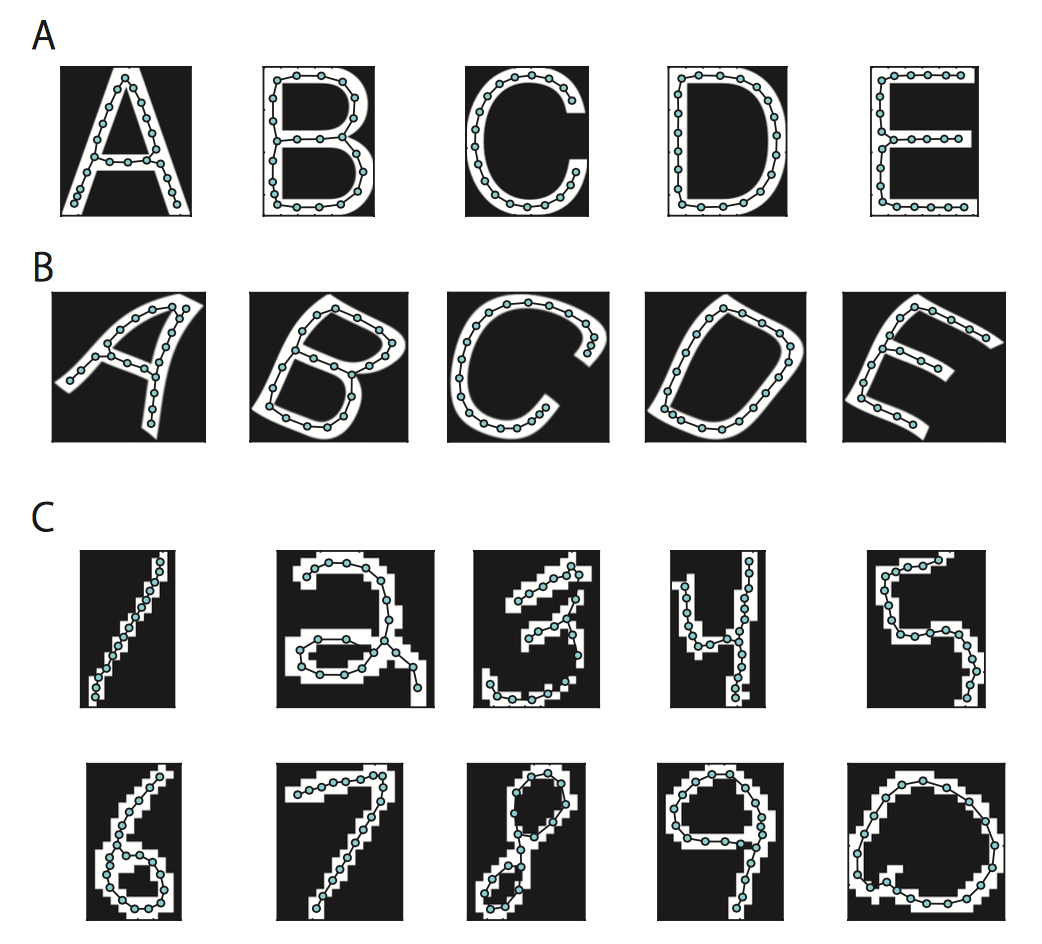
\includegraphics[width=1\linewidth]{../pictures/nn_skelet_ex.png}}
	\caption{
		Пример скелетирования символов (из работы~\cite{fujita2015extract}), соответствующих буквам латинского алфавита (A), наклонным буквам латинского алфавита (B) и цифрам (C). Цепочки на изображениях соответствуют результатам скелетирования.
        }
        \label{fig:nn_skelets}
\end{figure}
  
Вместо процедуры прореживания бинаризованного изображения, описанной выше, может быть применен альтернативный подход, называемый скелетированием изображений.
Скелетирование изображений также позволяет упростить последующий процесс извлечения существенных признаков изображения.
Суть данного метода заключается в замене исходной фигуры на изображении на однопиксельные линии, задающие общий контур фигуры.
Отметим работы~\cite{supriana2014handwriting} и~\cite{fujita2015extract} где для скелетирования объектов, представленных на изображении, используются современные методы машинного обучения такие как распространяющийся нейронный газ~\cite{fritzke1995growing} (growing neural gas, GNG) и метод относительных соседей на графе~\cite{toussaint1980relative} (relative neighborhood graph, RNG).
Также отметим работу~\cite{zou2003fast}, где для скелетирования предложен быстрый метод, использующий свойства симметрии объекта, и работу~\cite{zou2001skeletonization}, где для подавления артефактов скелетирования используются методы анализа точек регулярности и сингулярности формы.
В качестве примера, на рисунке~\ref{fig:nn_skelets} приводятся результаты процедуры скелетирования из работы~\cite{fujita2015extract}, примененной к символам латинского алфавита и к цифрам.
Как можно видеть, в результате скелетирования образуются однопиксельные кривые, сохраняющие общую информацию о форме исходного изображения.

В итоге, после успешного проведения всех описанных процедур, мы имеем очищенное от шума, бинаризованное изображение, на котором все линии имеют толщину не более одного пикселя.

\newpage
\subsection{Современные методы автоматического распознавания} \label{ss:captheory_methods}

В данном разделе мы рассмотрим наиболее современные методы машинного обучения в контексте задачи распознавания CAPTCHA.
Как уже неоднократно указывалось в работе, на сегодняшний день наиболее активно развивающимся направлением является нейросетевой подход.
Создано большое число новых архитектур ИНС, постоянно публикуются работы с новыми эвристиками выбора функций активации и функции стоимости.
В этом контексте, подробно рассмотренная в первом разделе работы полносвязная ИНС является лишь частным (и не всегда лучшим) случаем ИНС.
Однако полносвязные сети продолжают активно использоваться исследователями и инженерами.

При этом, естественным этапом в развитии метода ИНС стало увеличение их глубины, то есть последовательное расположение нескольких полносвязных слоев и иных типов слоев (с полным числом слоев даже более двадцати на сегодняшний день) для возможности иерархического анализа и выявления закономерностей во входных данных.
Такие ИНС называют глубокими (в литературе используется также термин <<глубинные>>) сетями, при этом отсутствует формальное ограничение на число слоев, начиная с которого сеть можно считать глубокой.
Так, в  качестве примера, на рисунке~\ref{fig:nn_deep}\footnote{
	Данное изображение заимствовано с веб-ресурса \url{http://searchnetworking.techtarget.com/definition/neural-network}.
}
схематически изображена полносвязная нейронная сеть с третями скрытыми слоями, которую можно считать глубокой ИНС.
Принцип действия такой сети не имеет принципиальных отличий от механизма работы полносвязной ИНС с одним скрытым слоем, описанной в первом разделе работы.
Входной слой передает без изменений входной вектор ИНС на первый внутренний слой.
Нейроны первого внутреннего слоя осуществляют преобразование сигнала в соответствии с текущими значениями весов и смещений.
Выходной сигнал затем подается на вход второго внутреннего слоя, где осуществляются аналогичные преобразования.
Затем аналогично сигнал обрабатывается третьим внутренним слоем и поступает на выходной слой сети.
После преобразования сигнала выходным слоем, получаем выходной вектор сети, являющийся ее предсказанием.

\begin{figure}[t!]
	\center{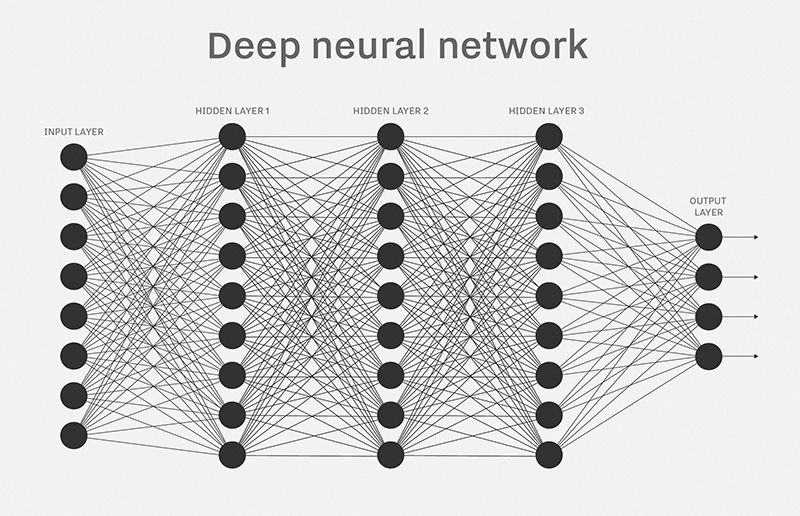
\includegraphics[width=1\linewidth]{../pictures/nn_deep.jpg}}
	\caption{
		Схематическое изображение полносвязной глубокой нейронной сети с тремя скрытыми слоями. Входной вектор $\vect{x}$ сети для данного примера имеет длину $8$, а выходной вектор $\vect{y}$ -- длину $4$.
        }
        \label{fig:nn_deep}
\end{figure}

Глубокие нейронные сети позволяют существенно повысить качество предсказаний сети.
На сегодняшний день отсутствует полное обоснование причин их эффективности, кроме интуитивного соображения, заключающегося в следующем факте.
Человеческому мозгу свойственна иерархичность восприятия.
Когда мы видим некоторый объект, то изначально светочувствительными элементами глаза воспринимаются отдельные точки изображения, затем нервной системой глаза производится первичная обработка сигнала: выделяются некоторые простые элементы (линии, углы).
Затем сигнал передается в мозг человека, где происходит дальнейшая последовательная обработка с введением все более сложных сущностей.
Аналогично глубокая ИНС при распознавании, например, лица человека на изображении может на первом внутреннем слое производить идентификацию некоторых простых форм (овалов, линий, углов), на следующем слое выявленные сущности могут усложняться (при наличии сигналов от нейронов предыдущего слоя, ответственных, например, за выявление овалов, может приниматься решение о наличии глаза на изображении) и далее от слоя к слою происходит дальнейшее усложнение сущностей, которое в итоге приводит к ответу сети о наличии или отсутствии лица на изображении.

Описанная иерархичность обработки входной информации, по всей видимости, и обеспечивает потрясающие результаты, которые глубокие ИНС демонстрируют в задачах распознавания и классификации.
Так например, глубокие сети с более чем тридцатью слоями используются в настоящее время для классификации популярного набора данных ImageNet~\cite{deng2009imagenet}.
Данная база содержит более $16$ миллионов полноцветных изображений, разбитых на $20$ тысяч категорий.
Задача, соответственно заключается в обучении сети предсказывать категорию заданного изображения.
Глубокие ИНС на сегодняшний день решают данную несоизмеримо лучше человека (см., например,~\cite{le2013building} и~\cite{ciregan2012multi}), верно определяя топ-5 категорий с точностью более $95\%$.
Отметим, что для описанной базы данных наиболее распространенная оценка качества сети -- это именно топ-5 категорий: рассматривается $5$ предсказаний категории, которые сеть считает наиболее вероятными, и если одно из них оказывается совпадающим с правильным, то такое предсказание считается верным.
Такой критерий оценки связен с тем фактом, что для огромного числа изображений практически невозможно (в том числе, человеку) точно определить категорию, например, для фотографии, на которой изображена собака и кошка, трудно выбрать между категориями <<собаки>> и <<кошки>>.
Добавим, что глубокие ИНС нашли на сегодняшний день ряд применений и в задачах распознавания речи на основе обработки отдельных звуков~\cite{hinton2012deep}, а также на основе специальных словарей~\cite{dahl2012context}.

Еще одно важное направление современного развития нейросетевого подхода -- это сверточные ИНС (convolutional neural network)~\cite{krizhevsky2012imagenet, szegedy2015going}.
Данный подход был разработан в последнее десятилетие и является естественным  обобщением метода классических ИНС, адаптированным для выявления закономерностей и работы с двухмерными и трехмерными входными структурами  данных, в частности, для работы с графическими изображениями.

\begin{figure}[t!]
	\center{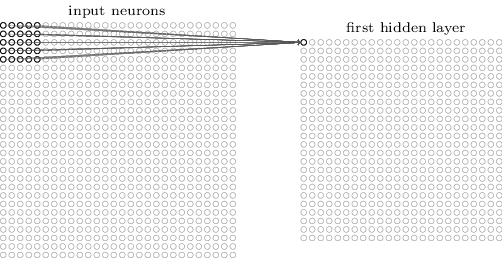
\includegraphics[width=1\linewidth]{../pictures/nn_conv_layer.png}}
	\caption{
		Схематическое изображение сверточного слоя ИНС.
        }
        \label{fig:nn_conv_layer}
\end{figure}

Основная идея здесь следующая.
Как описывалось в предыдущем разделе, для использования полносвязной ИНС в задаче распознавания изображений, необходимо векторизовать матрицу интенсивностей пикселей, то есть преобразовать ее в вектор, склеивая последовательно строки или столбцы исходной матрицы.
При этом неизбежно теряется часть информации связанной с двумерной структурой изображения, например, те пиксели, которые располагались рядом на изображении, в векторе уже могут оказаться на значительном удалении.
Для разрешения подобных проблем был предложен новый тип слоев ИНС - сверточный слой.
Данный слой также состоит из нейронов, однако они являются упорядоченными на плоскости в соответствии с геометрией исходного изображения.
В качестве примера на рисунке~\ref{fig:nn_conv_layer}\footnote{
	Данное изображение, а также изображения на рисунках~\ref{fig:nn_conv_layers} и~\ref{fig:nn_conv_net} заимствованы с веб-ресурса \url{http://neuralnetworksanddeeplearning.com/chap6.html}.
}
схематически изображен входной слой сверточной сети размера $28 \times 28$ (он может, например, соответствовать изображению размера $28 \times 28$) и следующий за ним сверточный слой.
Входной слой (input neurons на рисунке) соответствует значениям интенсивности пикселей изображения с учетом геометрии изображения.
Для получения сигнала сверточного слоя, находящегося за ним, выполняется следующая операция.
Выбирается некоторый размер окна (например, $5 \times 5$ пикселей, как изображено на рисунке), и выбираются соответствующие пиксели (нейроны), попадающие в данное окно.
Изначально (как изображено на рисунке) окно располагается в верхнем левом углу изображения.
Для всех нейронов, попавших в окно, вычисляется свертка по формуле
\begin{equation} \label{ss:captheory_methods_conv}
	\sigma 
		\left(
			b + \sum_{l=0}^{4} \sum_{m=0}^{4} w_{l,m} a_{i+l,j+m}
		\right),
\end{equation}
значение которой будет выходом $(i,j)$-ого нейрона сверточного слоя (для начального положения окна имеем соответственно $i=0$ и $j=0$).
Затем происходит сдвиг окна на один пиксель вправо и вновь вычисляется выход $(i,j)$-ого нейрона сверточного слоя (теперь $i=0$ и $j=1$) по формуле~\eqref{ss:captheory_methods_conv}.
Данный процесс продолжается до достижения правой границы изображения, затем происходит возврат к левой границе изображения со сдвигом на один пиксель вниз (что соответствует $i=1$ и $j=0$).

\begin{figure}[t!]
	\center{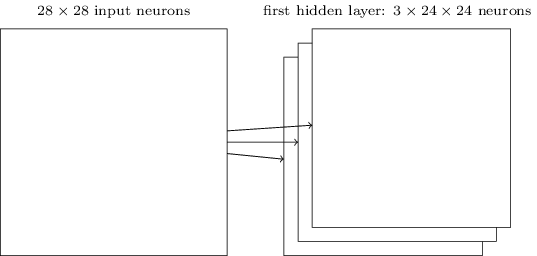
\includegraphics[width=1\linewidth]{../pictures/nn_conv_layers.png}}
	\caption{
		Схематическое изображение совокупности трех сверточных слоев ИНС.
        }
        \label{fig:nn_conv_layers}
\end{figure}

Поскольку на каждом шаге окно размера $5$ сдвигается на один пиксель, и при этом размер входного слоя для рассматриваемого примера $28 \times 28$, то в итоге сверточный слой, в соответствии с описанным алгоритмом, будет содержать $24 \times 24$ нейронов (так всего возможно $28-5+1=24$ положений окна по каждому из направлений).
При этом, в соответствии с формулой~\eqref{ss:captheory_methods_conv}, каждому положению окна соответствует одни и те же значения весов $w_{l,m}$ и смещения $b$, таким образом, сверточный слой имеет всего $26$ параметров.

Смысл введения сверточного слоя в соответствии с формулой~\eqref{ss:captheory_methods_conv} следующий.
Описанный обход входного слоя с помощью небольшого окна и малым сдвигом соответствует поиску некоторой (одной) особенности на изображении, например, это может быть поиск острого угла на картинке.
В данном контексте становится понятно, почему для каждого положения окна используются одни и те же веса и смещения -- конкретный сверточный слой нацелен на выявление конкретной особенности на изображении (в любом месте изображения).

\begin{figure}[t!]
	\center{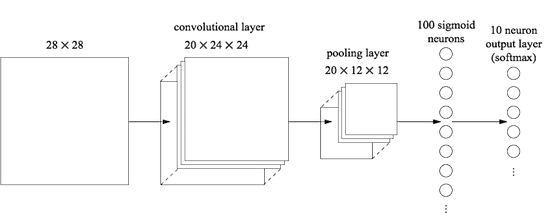
\includegraphics[width=1\linewidth]{../pictures/nn_conv_net.png}}
	\caption{
		Схематическое изображение ИНС, содержащей сверточные слои.
        }
        \label{fig:nn_conv_net}
\end{figure}

Поскольку один сверточный слой, как было описано выше, способен выявить только одну особенность, то логичным представляется параллельное использование нескольких сверточных слоев (корректнее -- подслоев, так все эти сверточные подслои располагаются в одном месте сети, как бы расширяя ее в дополнительном измерении), каждый из которых характеризуется своими весами и смещениями и нацелен на выявление некоторой особенности изображения.
На рисунке~\ref{fig:nn_conv_layers} приведен пример части ИНС со входным слоем и первым внутренним слоем, состоящим из трех сверточных подслоев.

В реальных приложениях сверточных подслоев в одном слое может быть существенно больше, чем три -- их число должно соответствовать количеству важных особенностей изображения.
Так в качестве примера, на рисунке~\ref{fig:nn_conv_net} изображена глубокая ИНС, содержащая сверточный слой, который, в свою очередь, состоит из $20$ подслоев, каждый из который выделяет одну характерную особенность на изображении.

\begin{figure}[t!]
	\center{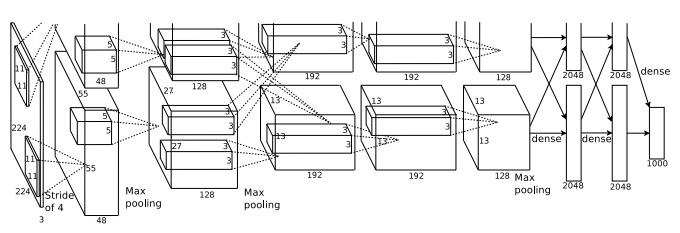
\includegraphics[width=1\linewidth]{../pictures/nn_real.jpg}}
	\caption{
		Пример реальной глубокой нейронной (из работы~\cite{krizhevsky2012imagenet}) для классификации изображений.
        }
        \label{fig:nn_real}
\end{figure}

На сегодняшний день ИНС, в том числе, со сверточными слоями, применяются в широком спектре приложений.
При этом сложность архитектуры современных ИНС достигла потрясающих масштабов.
На рисунке~\ref{fig:nn_real} изображена сверточная глубокая ИНС, использованная для классификации более чем миллиона изображений в высоком разрешении на $1000$ различных заданных классов в рамках популярного конкурса машинного обучения ImageNet, описанного выше.
Сеть имеет $650000$ нейронов, включая пять сверточных слоев и три полносвязных слоя, при этом сеть имеет более $60$ миллионов параметров.
Приведенный пример взят из работы~\cite{krizhevsky2012imagenet} 2010 года, и на сегодняшний день, безусловно, создаются и успешно обучаются существенно более сложные ИНС с еще большим числом параметров.

Чрезвычайно высокая сложность и требовательность к вычислительным ресурсам современных глубоких нейросетевых структур обуславливает необходимость разработки новых эффективных  подходов для обучения и функционирования сети.
Отметим, что обучение и функционирование являются двумя различающимися аспектами работы с современными сетями.
Так первичное обучение глубоких сетей обычно осуществляется с использованием суперкомьютеров и вычислительных кластеров на мощных графических процессорах, например, это может быть обучение сети, предсказывающей пробки на вычислительных системах Яндекса.
Обученная таким образом сеть далее может использоваться конкретными пользователями для получения соответствующих прогнозов (фаза функционирования), при этом запросы во многих случаях осуществляются с маломощных мобильных устройств (смартфоны, планшеты и т.д.).

На обоих приведенных этапах ИНС потребляет массу вычислительных ресурсов.
При этом обучение современных сетей может занимать недели и месяцы, а функционирование обученной сети на мобильном устройстве практически невозможно, поэтому для использования сети необходим постоянный доступ к сети Интернет: мобильное устройство делает запрос к серверу, на котором размещена сеть, делается предсказание, и результат отправляется обратно по сети.
Однако такая модель имеет ряд ограничений, в частности, необходимость наличия Интернет-соединения.
Яркий иллюстративный пример здесь -- это наблюдение за тем как <<глупеют>> электронные помощники с искусственным интеллектом (например, Siri) при потери доступа к сети Интернет.
Очевидное решение здесь -- это размещение обученных ИНС непосредственно на мобильных устройствах, однако для этого необходимы новые алгоритмы, позволяющие компактно представлять массивы весов сети и вычислительно эффективно проводить процедуру прямого распространения сигнала в сети.

Наиболее современный на сегодняшний день подход в рамках данного направления, на наш взгляд -- это методы тензоризации ИНС~\cite{novikov2015tensorizing, lebedev2014speeding, socher2013reasoning, yu2012large, yu2013deep, kim2015compression, janzamin2015beating}. 
Данное направление начало активно развиваться только лишь в последние 2-3 года, и основано на идее малопараметрических тензорных аппроксимаций.

Как было показано в работах~\cite{oseledets2010tt, oseledets2011tensor, savostyanov2011fast} во многих практически значимых случаях многомерные массивы (тензоры) могут быть представлены в компактной (малопараметрической или малоранговой) форме в рамках, так называемого, разложения тензорного поезда (tensor train decomposition).
Пусть $\tensor{X}$ -- это многомерный массив, имеющий $d$ измерений (при $d=2$ -- это матрица, а при $d=1$ -- вектор), с числом элементов $n$ вдоль каждого из измерений.
Как можно видеть, полное число элементов такого массива $n^d$, и уже при сравнительно небольших значениях $d$ и $n$ такие массивы становится невозможным хранить в памяти компьютеров (например, для четырехмерного массива с $1000$ элементов вдоль каждого измерения мы имеем полное число элементов $10^{12}$) -- так называемая проблема проклятия размерности.
Однако практически любой массив данных имеет некоторую внутреннюю структуру, при учете которой он может быть представлен в значительное более компактной форме.
В рамках разложения тензорного поезда многомерный массив $\tensor{X}$ путем многократного вычисления сингулярного разложения (SVD, см. Приложение~1) матриц-разверток, представляется в виде
$$
	\tensor{X} = \sum_{\alpha_1=1}^{r_1}  \sum_{\alpha_2=1}^{r_2} \ldots  \sum_{\alpha_{d-1}=1}^{r_{d-1}}
		\tensor{G}_1 (1, i_1, \alpha_1)
		\tensor{G}_2 ( \alpha_1, i_2, \alpha_2)
		\ldots
		\tensor{G}_d ( \alpha_{d-1}, i_d, 1),
$$
где $r_1, r_2, \ldots, r_{d-1}$ -- это ранги разложения, а трехмерные массивы $\tensor{G}_1, \tensor{G}_2, \ldots, \tensor{G}_d$ -- это, так называемые, ядра разложения.
Как можно видеть из приведенной формулы, полное число параметров в таком разложении не превосходит величины 
$$
	d \times n \times \max(r_k)^2,
$$
то есть линейно зависит от размерности и числа элементов вдоль каждого измерения при ограниченности рангов разложения.
В указанных работах было доказано, что ранги действительно являются ограниченными для широкого класса многомерных массивов, в частности, полученных из линейных комбинаций полиномиальных и тригонометрических функций и т.д.

Аналогичное разложение может быть применено также к матрицам и векторам, если они формально представлены в виде многомерных массивов путем процедуры тензоризации~\cite{oseledets2010approximation}. Для получаемых объектов потребляемая память и вычислительная сложность становится логарифмической по числу элементов, что позволяет в ряде случаев в тысячи раз снижать потребление памяти и вычислительных ресурсов.

В работе~\cite{novikov2015tensorizing} описанное разложение было применено для компактного представления полносвязного слоя ИНС, что позволило на порядок ускорить работу сети, а, например, в работе~\cite{lebedev2014speeding}, подобное разложение было использовано для представления сверточного слоя сети, что также в десятки раз улучшило ее производительность.

%=======================================================================
\newpage
\section{Реализация метода автоматического распознавания CAPTCHA} \label{s:soft}

\subsection{Введение} \label{ss:soft_intro}

В данной, заключительной, главе мы рассматриваем практические аспекты реализации программного комплекса для распознавания текстов на графических изображениях, в том числе для распознавания CAPTCHA.
В основе программного комплекса лежит полносвязная искусственная нейронная сеть (ИНС), принцип действия которой был рассмотрен в первой главе работы.
Для предварительной обработки изображения и сегментации его на отдельные символы мы используем методы, описанные во второй главе работы.

В разделе~\ref{ss:soft_nn} мы более подробно рассмотрим выбранную архитектуру ИНС и сформулируем алгоритмы обучения и функционирования, на основе которых будет разработана программная реализация.

Далее в разделе~\ref{ss:soft_package} мы детально описываем созданный программный пакет CapSolver для распознавания текста на графических изображениях, включая CAPTCHA, содержащий в качестве основных компонент модуль, реализующий полносвязную ИНС; модуль, реализующий загрузку, обработку и отображение изображений; браузерное расширение (плагин) для автоматического обнаружения поддерживаемой CAPTCHA на веб-странице, ее отправки на локальный сервер и автоматической вставки результата распознавания в соответствующее поле веб-страницы; локальный сервер и обработчики клиент-серверных сообщений и ряд вспомогательных модулей.
Браузерное расширение написано на языках html, css, javascript, а также использует специфическое API браузера Google Chrome.
Остальная часть кода создана с использованием языка программирования python 2.7 и ряда вспомогательных библиотек.

И наконец в разделе~\ref{ss:soft_results} мы приводим результаты практического применения программного пакета и особенности соответствующих наборов обучающих данных для конкретных задач распознавания, включая распознавание рукописных цифр из базы MNIST ($60000$ изображений в размеченной базе) и самостоятельно размеченной автором работы циферной CAPTCHA иностранного новостного портала.

\newpage
\subsection{Архитектура искусственной нейронной сети} \label{ss:soft_nn}

\begin{algorithm}[t]
	\caption{
		Алгоритм распространения сигнала в ИНС (forward).
	} \label{alg:nn_forw}
	\begin{algorithmic}[1]
    	\Require $\;$
    	
    		число слоев сети $L$;
    		
    		количества нейронов в слоях $N^{(0)}, N^{(1)}, \ldots, N^{(L-1)}$;
    		
    		матрицы весов нейронов $\matr{W}^{(1)}, \matr{W}^{(2)}, \ldots, \matr{W}^{(L-1)}$;
    		
    		векторы смещений нейронов $\vect{b}^{(1)}, \vect{b}^{(2)}, \ldots, \vect{b}^{(L-1)}$;
    		
    		функции активации для каждого из слоев $\sigma^{(1)}, \sigma^{(2)}, \ldots, \sigma^{(L-1)}$;
    		
    		входной вектор $\vect{x}$ размера $N^{(0)}$.
    		
		\State Задать векторы $\vect{z}^{(0)} = \vect{x}$ и $\vect{a}^{(0)} = \vect{x}$.
		\For{$l = 1, 2, \ldots, L-1$}
			\State Вычислить вектор $\vect{z}^{(l)} = \matr{W}^{(l)} \vect{a}^{(l-1)} + \vect{b}^{(l)}$.
			\State Вычислить вектор $\vect{a}^{(l)} = \sigma^{(l)} (\vect{z}^{(l)})$.
		\EndFor
		\Ensure  выходные векторы слоев $\vect{a}^{(0)}, \vect{a}^{(1)}, \ldots, \vect{a}^{(L-1)}$ 
		
		($\vect{a}^{(0)}$ совпадает со входом сети, $\vect{a}^{(L-1)}$ является выходным вектором сети).
	\end{algorithmic}
\end{algorithm}

\begin{algorithm}[t]
	\caption{
		Алгоритм одной эпохи обучения ИНС (backward).
	} \label{alg:nn_back}
	\begin{algorithmic}[1]
    	\Require $\;$
    	
    		число слоев сети $L$;
    		
    		количества нейронов в слоях $N^{(0)}, N^{(1)}, \ldots, N^{(L-1)}$;
    		
    		матрицы весов нейронов $\matr{W}^{(1)}, \matr{W}^{(2)}, \ldots, \matr{W}^{(L-1)}$;
    		
    		векторы смещений нейронов $\vect{b}^{(1)}, \vect{b}^{(2)}, \ldots, \vect{b}^{(L-1)}$;

    		функции активации для каждого из слоев $\sigma^{(1)}, \sigma^{(2)}, \ldots, \sigma^{(L-1)}$;
    		
    		функция стоимости одного измерения $C_{\vect{x}}$;
    		
			размер подвыборки $M^{(mb)}$;
			
			параметр скорости обучения $\eta$;
			
    		набор обучающих данных $(\vect{x}_{q}, \vect{y}_{q})$ ($q= 0, 1, \ldots, M^{(trn)}-1$).
    		
		\State Задать матрицы $\Delta \matr{W}^{(1)}, \Delta  \matr{W}^{(2)}, \ldots, \Delta \matr{W}^{(L-1)}$, заполненные нулями, и имеющие формы, совпадающие с $\matr{W}^{(1)}, \matr{W}^{(2)}, \ldots, \matr{W}^{(L-1)}$ соответственно.
		\State Задать векторы $\Delta \vect{b}^{(1)}, \Delta  \vect{b}^{(2)}, \ldots, \Delta \vect{b}^{(L-1)}$, заполненные нулями, и имеющие размер, совпадающий с $\vect{b}^{(1)}, \vect{b}^{(2)}, \ldots, \vect{b}^{(L-1)}$ соответственно.
		\For{$q = 0, 1, \ldots, M^{(mb)}-1$}
			\State Используя равномерное случайное распределение, получить случайное число $r(q)$ ($0 \leq r(q) < M^{(mb)}$) и выбрать соответствующий элемент $(\vect{x}_{r(q)}, \vect{y}_{r(q)})$ из обучающей выборки данных.
			\State Вычислить выходные векторы слоев сети $\vect{a}^{(0)}, \vect{a}^{(1)}, \ldots, \vect{a}^{(L-1)}$, соответствующие входному вектору сети $\vect{x}_{r(q)}$, используя функцию forward из алгоритма~\ref{alg:nn_forw}.
			\State Вычислить вектор ошибки последнего слоя 
			$\vect{\delta}^{(L-1)} = \frac{\partial C_{\vect{x}}}{\partial \vect{a}^{(L-1)}} \odot \sigma'(\vect{z}^{(L-1)})$.
			\For{$l = L-2, L-3, \ldots, 1$}
				\State Вычислить вектор ошибки $l$-ого слоя 
				$\vect{\delta}^{(l)} = \left( \left( \matr{W}^{(l+1)} \right)^T \vect{\delta}^{(l+1)} \right) \odot \sigma'(\vect{z}^{(l)})$.
				\State Обновить значение 
				$\Delta \vect{b}^{(l)} = \Delta \vect{b}^{(l)}  + \vect{\delta}^{(l)}$.
				\State Обновить значение 
				$\Delta \matr{W}^{(l)} = \Delta \matr{W}^{(l)}  + \vect{\delta}^{(l)} \left( \vect{a}^{(l-1)} \right)^T$.
			\EndFor
		\EndFor
		\For{$l =1, 2, \ldots, L-1$}
			\State Обновить значение $\vect{b}^{(l)} = \vect{b}^{(l)} - \frac{\eta}{M^{(mb)}} \Delta \vect{b}^{(l)}$.
			\State Обновить значение $\matr{W}^{(l)} = \matr{W}^{(l)} - \frac{\eta}{M^{(mb)}} \Delta \matr{W}^{(l)}$.
		\EndFor
		\Ensure обновленные матрицы весов нейронов $\matr{W}^{(1)}, \matr{W}^{(2)}, \ldots, \matr{W}^{(L-1)}$ и векторы смещений нейронов $\vect{b}^{(1)}, \vect{b}^{(2)}, \ldots, \vect{b}^{(L-1)}$.
	\end{algorithmic}
\end{algorithm}

\begin{algorithm}[t]
	\caption{
		Алгоритм обучения ИНС (learning).
	} \label{alg:nn_learning}
	\begin{algorithmic}[1]
    	\Require $\;$
    	
    		число слоев сети $L$;
    		
    		количества нейронов в слоях $N^{(0)}, N^{(1)}, \ldots, N^{(L-1)}$;
    		
    		матрицы весов нейронов $\matr{W}^{(1)}, \matr{W}^{(2)}, \ldots, \matr{W}^{(L-1)}$;
    		
    		векторы смещений нейронов $\vect{b}^{(1)}, \vect{b}^{(2)}, \ldots, \vect{b}^{(L-1)}$;

    		функции активации для каждого из слоев $\sigma^{(1)}, \sigma^{(2)}, \ldots, \sigma^{(L-1)}$;
    		
    		функция стоимости одного измерения $C_{\vect{x}}$;
    		
			размер подвыборки $M^{(mb)}$;
			
			параметр скорости обучения $\eta$;

    		набор обучающих данных $(\vect{x}_{q}, \vect{y}_{q})$ ($q= 0, 1, \ldots, M^{(trn)}-1$).
    		
    		набор тестовых данных $(\vect{x}_{t}, \vect{y}_{t})$ ($t= 0, 1, \ldots, M^{(tst)}-1$).
    		
   			максимальное количество эпох обучения $M^{(ep)}$;
   			
		\State Создать пустой список $acc$ для значений точности сети на каждой из эпох.
		\For{$e = 0, 1, \ldots, M^{(ep)}-1$}
			\State Провести одну эпоху обучения на обучающем наборе данных, используя функцию backward из алгоритма~\ref{alg:nn_back}.
			\State Создать и вещественную переменную $count$ и задать $count=0$.
			\For{$t = 0, 1, \ldots, M^{(tst)}-1$}
				\State Вычислить выходной вектор сети $\vect{a}^{(L-1)}$, соответствующий входному вектору сети $\vect{x}_{t}$ из тестового набора данных, используя функцию forward из алгоритма~\ref{alg:nn_forw}.
				\If $\vect{a}^{(L-1)}$ равно  $\vect{y}_{t}$
					$count = count + 1$ 
				\EndIf
			\EndFor
			\State Добавить в список $acc$ процент правильных ответов сети на данной эпохе $\frac{count}{M^{(tst)}}$.
		\EndFor
		\Ensure Матрицы весов нейронов $\matr{W}^{(1)}, \matr{W}^{(2)}, \ldots, \matr{W}^{(L-1)}$ и векторы смещений нейронов $\vect{b}^{(1)}, \vect{b}^{(2)}, \ldots, \vect{b}^{(L-1)}$ обученной сети, а также список точностей на каждой из эпох обучения $acc$.
	\end{algorithmic}
\end{algorithm}

Основным этапом при решении задачи автоматизированного распознавания символов и CAPTCHA является создание и обучение классификатора, позволяющего распознавать конкретные символы в режиме онлайн на основе результатов предварительного обучения в режиме офлайн на размеченной обучающей выборке данных.
В случае распознавания текстовой информации на графических изображениях элементами обучающей выборки являются пары $\vect{x}, \vect{y}$, где $\vect{x}$ -- это определенным образом упорядоченный массив интенсивностей отдельных пикселей изображения, а $\vect{y}$ -- это желаемый выход классификатора, то есть правильное значение символа, представленного на изображении.

Ранее в данной работе были описаны преимущества нейросетевого подхода для решения задач классификации.
Для автоматизации процесса распознавания CAPTCHA нами была реализована полносвязная ИНС, принцип действия которой подробно описывается в разделе~1 данной работы.
Прямое распространение сигнала в сети может быть реализовано в форме функции forward, представленной в виде псевдокода в алгоритме~\ref{alg:nn_forw}.
Данная функция принимает текущие значения параметров сети (весов и смещений всех нейронов), а также использует гиперпараметры сети (число слоев, количества нейронов в слоях, функции активации для каждого из слоев).
По заданному входному вектору функция вычисляет и возвращает выходы всех слоев сети, при этом выход последнего слоя сети является выходом (предсказанием) сети, а выходы остальных слоев необходимы для работы алгоритма обучения сети.

В алгоритме~\ref{alg:nn_back} представлен псевдокод функции backward, осуществляющей одну эпоху обучения ИНС с использованием метода стохастического градиентного спуска и метода обратного распространения ошибок, описанных в разделе~1 данной работы.

При программной реализации алгоритма для каждого из слоев необходимы две функции: одна вычисляет значение функции активации, а вторая -- ее производную по заданному взвешенному выходу нейрона (или всего слоя).

Фактически для работы алгоритма необходима только частная производная функции стоимости по выходному вектору сети $\frac{\partial C_{\vect{x}}}{\partial \vect{a}^{(L-1)}}$, соответственно, при программной реализации алгоритма необходима функция cost\_function\_der\_a(a, y), которая по заданному выходному вектору сети и по желаемому выходу (который известен для данных из обучающей выборки), вычисляет соответствую частную производную.

В соответствии с представленным в разделе~\ref{s:review} алгоритмом обучения ИНС, гиперпараметрами сети являются: 
\begin{itemize}
	\item число слоев ($L$),
	\item количество нейронов в каждом из внутренних слоев\footnote{
		Количество нейронов во входном слое ($N^{(0)}$) определяется фиксированной размерностью входного вектора, а количество нейронов в выходном слое ($N^{(L-1)}$) -- фиксированной размерностью выходного вектора.
	}
	($N^{(1)}, N^{(2)}, \ldots, N^{(L-2)}$),
	\item метод выбора начальных (случайных) значений весов нейронов ($\matr{W}^{(1)}, \matr{W}^{(2)}, \ldots, \matr{W}^{(L-1)}$) и смещений нейронов ($\vect{b}^{(1)}, \vect{b}^{(2)}, \ldots, \vect{b}^{(L-1)}$),
	\item вид функции активации каждого из слоев, кроме входного ($\sigma^{(1)}, \sigma^{(2)}, \ldots, \sigma^{(N-1)}$),
	\item вид функции стоимости отдельного измерения ($C_{\vect{x}}$),
	\item размер подвыборки ($M^{(mb)}$),
	\item параметр скорости обучения ($\eta$),
	\item количество эпох обучения ($M^{(ep)}$).
\end{itemize}

Отметим, что в данной работе нами были выбраны популярные и широко используемые сигмоидальная (логистическая) функция активации вида
$$
	\sigma(z) = \frac{1}{1+e^{-z}},
$$
и квадратичная функция стоимости вида
\begin{equation} 
	C_{\vect{x}} = 
		\frac{1}{2} || \vect{y} - \vect{a}^{(L-1)} ||^2 =
		\frac{1}{2} \sum_{j=0}^{N^{(L-1)}-1} \left( \vect{y}[j] - \vect{a}^{(L-1)}[j] \right)^2.
\end{equation}

\newpage
\subsection{Программный пакет для распознавания CAPTCHA} \label{ss:soft_package}

Для автоматического распознавания CAPTCHA был создан программный пакет CapSolver, включающий в себя следующие основные компоненты:
\begin{itemize}
	\item модуль, реализующий полносвязную ИНС, включая процесс обучения и функционирования (папка $neural\_network$);
	\item модуль, реализующий загрузку изображений (из тестовой базы, из файла и из сети Интернет), их обработку и отображение (папка $image$);
	\item браузерное расширение (плагин) для автоматического обнаружения поддерживаемой CAPTCHA на веб-странице, ее отправки на локальный сервер и автоматической вставки результата распознавания в соответствующее поле веб-страницы (папка $cap\_plugin$);
	\item локальный сервер, осуществляющий связь с браузерным расширением (файл $server$);
	\item обработчик клиент-серверных сообщений (файл $message$);
	\item главный обработчик, взаимодействующий с локальным сервером и запускающий процесс распознавания CAPTCHA по запросу браузерного расширения (файл $manager$);
	\item рабочие ipython-блокноты для локального обучения, сохранения и тестирования ИНС для распознавания цифр из базы MNIST и распознавания циферной CAPTCHA (файл $cap\_recognition$);
	\item различные вспомогательные функции (файл $utils$).
\end{itemize}

\begin{figure}[t!]
	\center{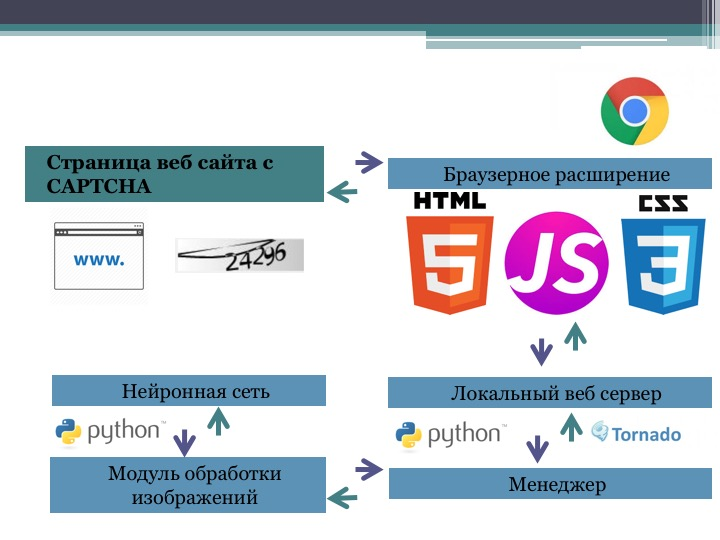
\includegraphics[width=1\linewidth]{../pictures/cap_solver.jpg}}
	\caption{
		Схематическое изображение логики работы разработанного программного комплекса CapSolver.
        }
        \label{fig:cap_solver}
\end{figure}

На рисунке~\ref{fig:nn_result_err} схематически представлен принцип работы программного комплекса.
При загрузке в веб браузере страницы сайта, содержащей поддерживаемую CAPTCHA, в автоматическом режиме происходит ее обнаружение, и на локальный сервер посредством технологии веб сокетов отправляет ссылка на изображение с указанием его типа.
Сервер при получении очередного сообщения передает его обработчику, который в свою очередь передает изображение модулю обработки изображения.
Здесь происходит удаление шумов, бинаризация и сегментация изображения на отдельные символы.
Далее символы последовательно передаются на распознавание предварительно обученной искусственной нейронной сети.
Результаты распознавания собираются обработчиком (менеджером) и далее при помощи сервера отправляются в плагин (браузерное расширение) по сети.
Полученный результат распознавания плагин автоматически вставляет в соответствующее поле веб страницы, предназначенное для ответа на заданную CAPTCHA.
При этом в текущей реализации время необходимое на распознавание символов и на совершение передачи на сервер и обратно в сумме составляет не более секунды.
Для возможности работы плагины и взаимодействия с локальным сервером при использовании протокола https на целевой странице, был реализован самоподписанный сетевой сертификат.

На всех этапах работы программного комплекса организован контроль ошибок.
При этом роль управляющего центра в текущей реализации играет сервер: при возникновении исключений на стороне браузерного расширения, на сервер отправляется соответствующее сообщение с описанием ошибки, и далее сервер принимает решение о продолжении работы либо об окончании текущего сокет-соединения.
При невозможности отправки сообщения на сервер, браузерное расширение отправляет сообщения в интерактивную консоль браузера.

\newpage
\subsection{Результаты практического применения программного пакета} \label{ss:soft_results}

\begin{figure}[t!]
	\center{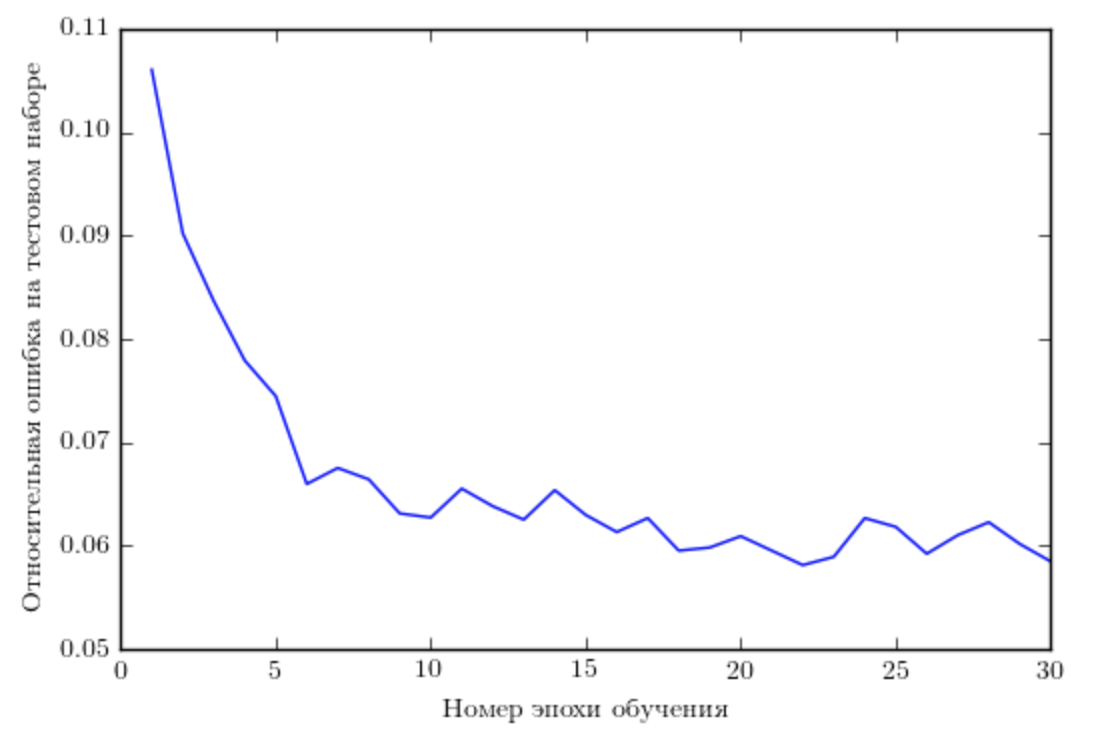
\includegraphics[width=1\linewidth]{../pictures/nn_result_err.png}}
	\caption{
		Относительная ошибка полносвязной ИНС при обучении на выборке из базы MNIST.
        }
        \label{fig:nn_result_err}
\end{figure}

\begin{figure}[t!]
	\center{
\includegraphics[width=1\linewidth]{../pictures/cap_site_part.png}}
	\caption{
		Пример поля для ввода CAPTCHA, к которой применялось автоматическое распознавание.
        }
        \label{fig:cap_site_part}
\end{figure}

\begin{figure}[t!]
	\center{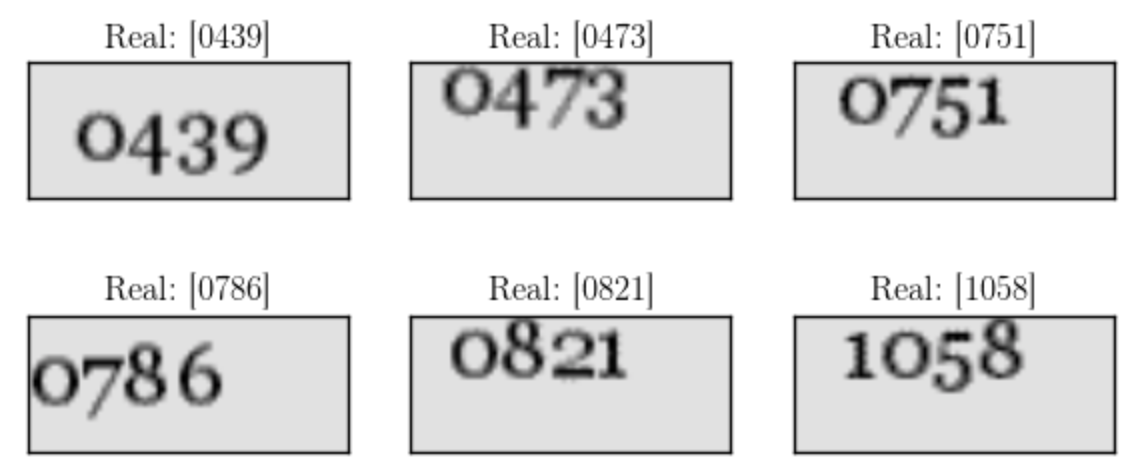
\includegraphics[width=1\linewidth]{../pictures/cap_site_recd.png}}
	\caption{
		Пример распознанных вручную CAPTCHA.
        }
        \label{fig:cap_site_recd}
\end{figure}

\begin{figure}[t!]
	\center{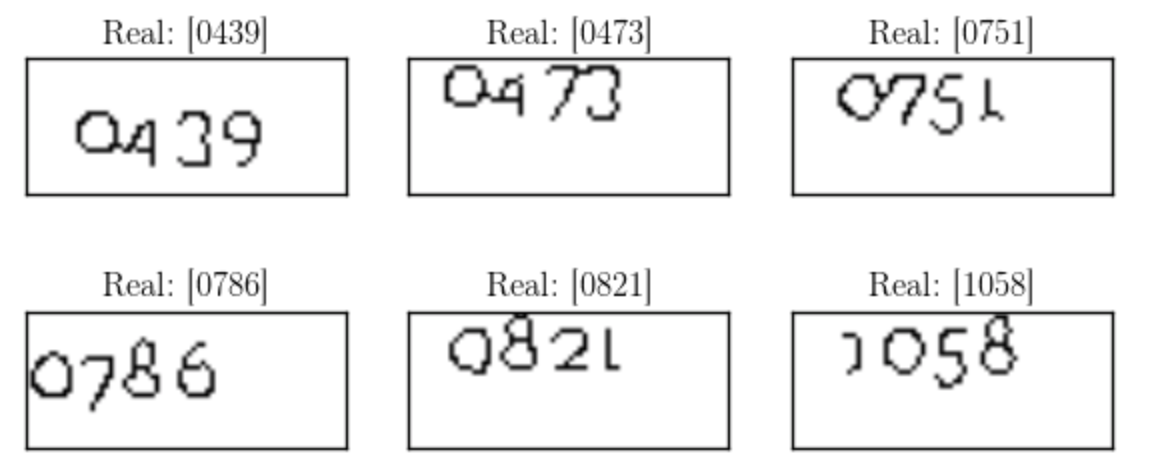
\includegraphics[width=1\linewidth]{../pictures/cap_site_skelet.png}}
	\caption{
		Пример CAPTCHA утоньщенных до одного пикселя.
        }
        \label{fig:cap_site_skelet}
\end{figure}

\begin{figure}[t!]
	\center{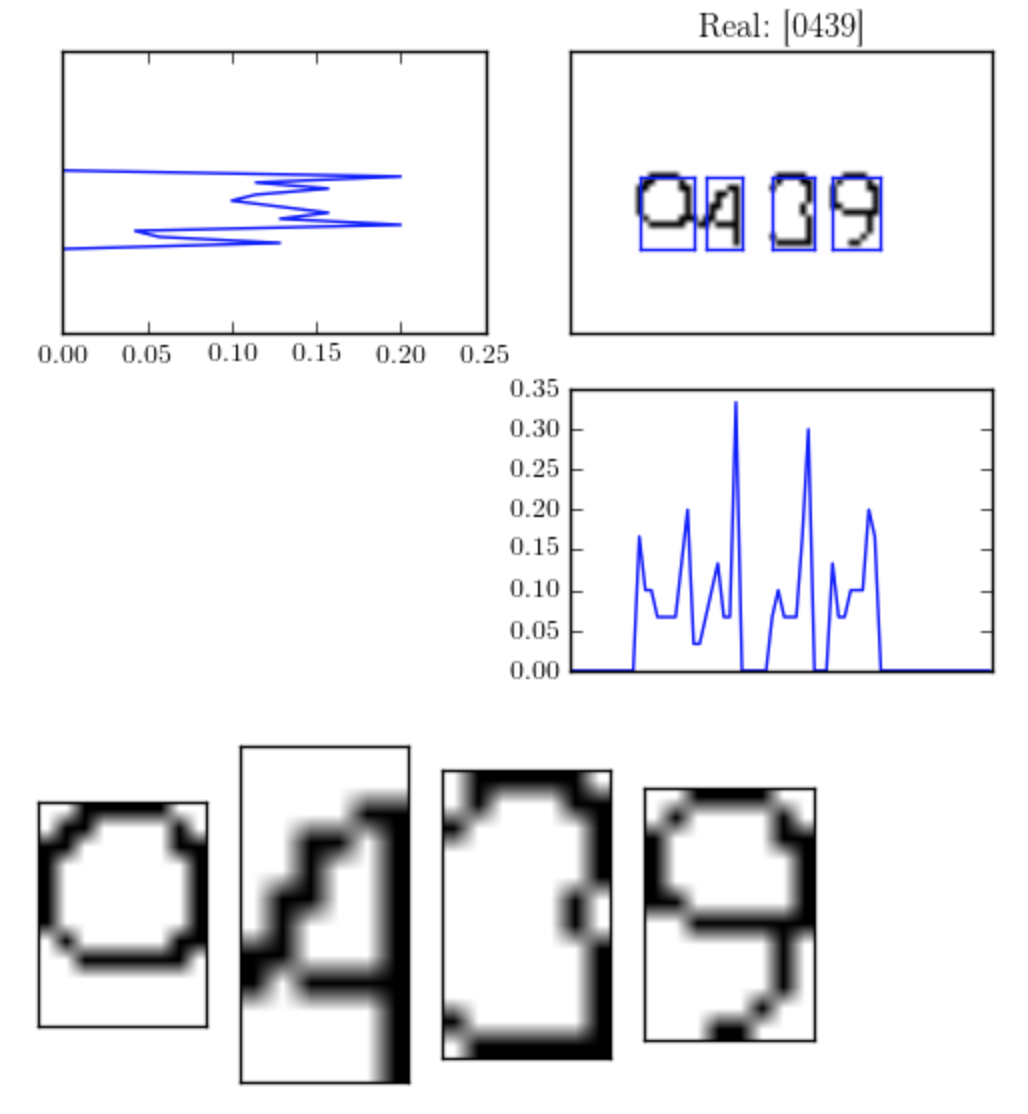
\includegraphics[width=1\linewidth]{../pictures/cap_site_segm.png}}
	\caption{
		Пример сегментированной CAPTCHA.
        }
        \label{fig:cap_site_segm}
\end{figure}



Для тестирования созданного программного комплекса нами было рассмотрено два класса задач.
Разработанная архитектура полносвязной искусственной нейронной сети и соответствующих алгоритмов очистки изображений от шума были протестированы на базе данных из предварительно распознанных рукописных символов MNIST.
Данная база содержит $7000$ распознанных изображений рукописных цифр, написанных различными людьми.
В первой части работы нами уже обсуждалась данная база и приводились примеры соответствующих изображений, поэтому здесь мы данное рассмотрение опускаем.

Нейронная сеть обучалась на $50000$ тестовых изображениях, для тестирования результатов обучения использовалось $10000$ изображений на этапе валидации, и затем $20000$ изображений.
Для оптимизации выбора гиперпараметров сети нами были проведена ее валидация на наборе из $10000$ размеченных изображений.
Итоговый выбор, комбинирующий удовлетворительную точность предсказаний при адекватном времени обучении (на настольном компьютере с использование CPU) был: $3.0$ для параметра скорости обучения, $1$ внутренний слой сети с $30$ нейронами, размер подвыборки для метода стохастического градиентного спуска был выбран равным $10$, а обучение происходило на протяжении $30$ эпох.

На рисунке~\ref{fig:nn_result_err} представлен график зависимости относительной доли ошибок сети на тестовом наборе данных в зависимости от текущей эпохи обучения.
В Приложении Б данной работы более подробно представлена практическая реализации обучения сети.

Для тестирования работы программного комплекса с реальными изображениями CAPTCHA, нами был выбран иностранный новостной ресурс \url{https://www.0629.com.ua/catalog/add}, требующий ввода циферной CAPTCHA при регистрации либо отправке комментария к новости.
На рисунке~\ref{fig:cap_site_part} приводится вид данной CAPTCHA, а на рисунке~\ref{fig:cap_site_recd} несколько примеров распознанных вручную CPATCHA.

Обучение нейросетевого классификатора производилось по самостоятельно размеченной выборке из $1000$ символов.
Для успешного автоматического распознавания данного вида CAPTCHA необходимо произвести последовательно:
\begin{enumerate}
	\item определить фоновые и текстовые наборы цветов и произвести бинаризацию изображения;
	\item произвести утоньшение (скелетонизацию изображения) c использованием алгоритмов из раздела 2 данной работы (Zhang-Suen thinning algorithm), см. рис.~\ref{fig:cap_site_skelet};
	\item произвести сегментацию полученного изображения, см. рис.~\ref{fig:cap_site_segm} - для данного типа CAPTCHA нами использовался простой алгоритм обрезания по порогу гистограммы, дающий точность около $85\%$;
	\item полученные в результате сегментации изображения распознаются полносвязной искусственной нейронной сетью по аналогии с изображениями из базы MNIST, при этом мы имеем точность около $80\%$ для отдельного символа.
\end{enumerate}

%=======================================================================
\newpage
\section*{ЗАКЛЮЧЕНИЕ}
\addcontentsline{toc}{section}{ЗАКЛЮЧЕНИЕ}

В работе нами были рассмотрены современные методы машинного обучения и интеллектуального анализа данных в контексте применения к задачам автоматического распознавания текстовой информации на графических изображениях.
В качестве основного метода нами был выбран нейросетевой подход, а в качестве задачи распознавания рассматривалось автоматическое распознавание (<<взлом>>) CAPTCHA.

Как было продемонстрировано в работе, наиболее перспективным на сегодняшний день направлением в области машинного обучения является метод искусственных нейронных сетей.
Регулярно публикуется большое число работ, посвященных новым архитектурам сетей и модификациям алгоритмов обучения.
Широкое распространение, особенно в контексте задачи обработки графических изображений, за последние несколько лет получили глубокие сверточные нейронные сети, которые были описаны в данной работе.

Одним из основных преимуществ метода искусственных нейронных сетей является практически полная универсальность, то есть единый подход к задачам из различных предметных областей: сбор размеченной обучающей выборки данных, выбор архитектуры и других гиперпараметров сети и, собственно, обучение сети в автоматическом режиме.
Появление больших объемов размеченных данных и мощных вычислительных средств обусловило возможность реального применения нейросетевого подхода в практических приложениях, включая задачи обработки изображений и текста, автоматизированные системы поддержки принятия решений в технических и медицинских приложениях и т.д.

Современные глубокие искусственные нейронные сети насчитывают миллионы параметров и требуют для своего обучения недели и месяцы.
Дальнейшее развитие метода искусственных нейронных сетей, как обсуждалось в работе, связано с созданием новых архитектур и алгоритмов обучения, позволяющих снизить вычислительную сложность и потребляемую память при обучении и функционировании сети.
Многообещающим подходом является, в частности, метод тензоризации сетей, в котором матрицы весов нейронных слоев представляются в малопараметрическом (сжатом) формате.
Подобные подходы позволят использовать обученные сети на мобильных и настольных устройствах без необходимости обращения к серверу, что приведет к еще большему распространению интеллектуальных программных систем (персональные помощники такие как Siri, локальные приложения для обработки изображений, системы для построения оптимальных маршрутов и др.).

Нейросетевой подход в применении к задачам распознавания CAPTCHA позволяет получать удовлетворительные результаты, как следует из анализа литературы, проведенного в работе.
Так для ряда типов CAPTCHA успешность распознавания может доходить до $90\%$.
С научной точки зрения, основная цель при построении подобных автоматических систем распознавания -- это выявление узких мест существующих алгоритмов распознавания и выработка рекомендаций по их улучшению.
По результатам проведенного в данной работе анализа литературы и практической реализации автоматической системы распознавания можно отметить, что при реализации CAPCTHA для повышения ее взломоустойчивости необходимо
\begin{itemize}
	\item в качестве текста использовать сочетания из цифровых и буквенных (в обоих регистрах) символов;
	\item избегать использования в качестве текста существующих словарных слов;
	\item использовать трансформации символов, в частности, повороты, неоднородные искажения и смещения по вертикали;
	\item реализовывать слабо повторяющееся расположение символов по горизонтали, а также использовать тексты переменной длины;
	\item использовать шумовые линии, пересекающие текст CAPTCHA, а также выходящие за пределы текста. 
\end{itemize}

Отметим, что в задаче разработки CAPTCHA помимо требования устойчивости к автоматизированному взлому, возникает второе, не менее важное требование -- возможность быстрого распознавания CAPTCHA человеком.
То есть CAPTCHA должна легко разгадываться человеком, но иметь высокую сложность для автоматического распознавания роботом.
И в этом контексте, сформулированные выше требования по взломоустойчивости часто не могут быть применены в полной мере ввиду усложнения итоговой CAPTCHA для восприятия человеком.
На сегодняшний день начинают получать распространение системы аналогичные по задаче CAPTCHA, но построенные на основе интеллектуального анализа (с использованием нейросетевого подхода) истории поисковых запросов и иной информации о конкретном пользователе для принятия окончательного решения человек/робот.
Однако пока что такие системы не являются достаточно надежными и в большинстве случаев все равно требуют разгадывания CAPTCHA (при сомнениях в <<человечности>> посетителя веб-ресурса).

На основе нейросетевого подхода в работе был разработан программный комплекс для автоматического распознавания CAPTCHA.
В данном комплексе были использованы полносвязные искусственные нейронные сети и ряд алгоритмов для предварительной обработки и сегментации изображений с текстовой информацией.
Для тестирования комплекса нами была рассмотрена задача распознавания рукописных цифр из популярной базы MNIST, содержащей $60000$ изображений цифр, написанных различными людьми.
Точность распознавания на тестовой выборке из $10000$ изображений составила $95\%$.

Верификация комплекса проводилась на задаче автоматического распознавания циферной CAPTCHA.
Точность сегментации изображения на отдельные символы в данном случае составила $30\%$, а точность распознавания отдельного символа $70\%$.
Для возможности практического использования данного комплекса  было разработано браузерное расширение (plugin), которое автоматически обнаруживает поддерживаемую CAPTCHA на веб-странице, отправляет изображение на локальный сервер и автоматически вводит полученный результат распознавания в соответствующее поле.
Отметим, что не смотря на недостаточно высокую точность распознавания в текущей версии программного комплекса, он может быть удобным для ускорения процесса разгадывания CAPTCHA человеком: пользователю достаточно просто при необходимости подкорректировать результат автоматического распознавания, то есть комплекс в данном случае выступает как система типа <<второе мнение>>.

Проделанная работа имеет ряд естественных направлений дальнейшего развития, включая:
\begin{enumerate}
	\item улучшение используемой нейросетевой архитектуры, в частности, переход к глубоким сверточным искусственным нейронным сетям;
	\item развитие алгоритмов предобработки и сегментации изображений;
	\item обучение комплекса распознаванию различных типов распространенных CAPTCHA;
	\item развитие созданного браузерного расширения, в частности, дополнение его развитым пользовательским интерфейсом, добавление системы аутентификации пользователя и т.д.;
	\item применение разработанного подхода к распознаванию иных типов графических изображений, включая тексты, автомобильные номера, дорожные знаки и др.
\end{enumerate}

%=======================================================================
\newpage
\addcontentsline{toc}{section}{СПИСОК ИСПОЛЬЗОВАННЫХ ИСТОЧНИКОВ}
\renewcommand\refname{\Large\centering СПИСОК ИСПОЛЬЗОВАННЫХ ИСТОЧНИКОВ}
\bibliography{biblio}

%=======================================================================
\newpage
\section*{ПРИЛОЖЕНИЕ А. Сингулярное разложение} \label{app:svd}
\addcontentsline{toc}{section}{ПРИЛОЖЕНИЕ А. Сингулярное разложение}

Для вычисления собственных чисел и собственных векторов (спектра) симметричной матрицы~\cite{tirt_matix}, а также для построения малорангового (малопараметрического) приближения матрицы может быть использован метод сингулярного разложения (singular value decomposition, SVD)~\cite{svd}.
	
Для произвольной матрицы $\matr{A}$ размера $m \times n$, заданной на поле вещественных или комплексных чисел, рассмотрим эрмитово сопряженную с ней матрицу $\matr{A}^*$, которая может быть получена из исходной матрицы путем ее транспонирования и замены всех элементов на комплексно сопряженные. 
Тогда матричное произведение $\matr{A}^* \matr{A}$ оказывается эрмитовой ($ \left( \matr{A}^* A \right) ^* = \matr{A}^* \matr{A}$) неотрицательно определенной ($\vect{x}^T \matr{A}^* \matr{A} \vect{x} \geq 0, \; \forall \vect{x} \in R^{n} $) матрицей размера $n \times n$. 
Как известно, все собственные значения такой матрицы неотрицательны, а собственные векторы образуют ортонормированный базис. 
	
Сингулярными числами матрицы $\matr{A}$ называют квадратные корни из собственных значений матрицы $\matr{A}^* \matr{A}$, отсортированных по неубыванию и обозначают $\sigma_i$ или $\sigma_i(\matr{A})$, где $i=1,\ldots,n$.
Имеем, соответственно,
$$
	\sigma_1 \geq \sigma_2 \geq \ldots \geq \sigma_r > \sigma_{r+1} = \ldots = \sigma_{n} = 0.
$$
В соответствии с данным представлением, матрица $\matr{A}$ имеет ровно $r$ ненулевых сингулярных чисел ($r$ может в некоторых случаях совпадать с $n$).

	Пусть $\bm{u_1}, \ldots, \bm{u_n}$ - ортонормированный базис, состоящий из собственных векторов матрицы $A^*A$, причем, нумерация выбрана так, что
	\begin{equation}\label{SVD_vect}
		\begin{split}
			& A^*A \bm{u_i} = \sigma_i^2 \bm{u_i}, \;\; 1   \leq i \leq r, \\
			& A^*A \bm{u_i} = 0                  , \;\; r+1 \leq i \leq n. 
		\end{split}
	\end{equation}
	
	Отметим, что при $i \geq r+1$ выполняется:
	\begin{equation}\label{SVD_spec}
		A^*A \bm{u_i} = 0 \longrightarrow \bm{u_i^*} A^*A \bm{u_i} = 0 \longrightarrow A \bm{u_i} = 0.
	\end{equation}
	
	Введем систему векторов 
	\begin{equation}\label{SVD_v}
		\bm{v_i}=\frac{A\bm{u_i}}{\sigma_i}, \;\; i=1,\ldots,r.
	\end{equation}
	
	Для такой системы векторов выполняется: 
	\begin{equation}\label{SVD_vect_syst}
		\begin{split}
			& \bm{v_i}^T \bm{v_j} = 0, \;\; 1   \leq i,j \leq r, \;\; i \neq j,\\
			& \bm{v_i}^T \bm{v_i} = 1, \;\; 1   \leq i \leq r. 
		\end{split}
	\end{equation}
	
	Система из $r$ векторов $\bm{v_i}$, $i=1,\ldots,r$ может в этом случае быть дополнена векторами $\bm{v_{r+1}}, \ldots, \bm{v_{m}}$ до ортонормированного базиса в $m$-мерном пространстве.
	
	Соответственно, с учетом \ref{SVD_spec} и \ref{SVD_v} получаем:
	\begin{equation}\label{SVD_vect_syst}
		\begin{split}
			& A \bm{u_i} = \bm{v_i} \times \sigma_i, \;\; i=1,\ldots,r, \\
			& A \bm{u_i} = \bm{v_i} \times 0       , \;\; i=r+1,\ldots,n. 
		\end{split}
	\end{equation}
	
	В матричной форме последнее соотношение может быть записано как
	\begin{equation}\label{SVD_1}
	A U = V S,
	\end{equation}
	где	эрмитовы (в вещественном случае - ортогональные) матрицы $U$ и $V$ ($U^* = U^{-1}$ и $V^* = V^{-1}$) получены объединением столбцов, соответствующих системам векторов $\bm{u_i}$ и $\bm{v_i}$, а $S$ -диагональная матрица из сингулярных векторов, имеющая тот же размер, что и матрица $A$: 
	\begin{equation}\label{SVD_UV}
		\begin{split}
			& U_{n \times n} = [\bm{u_1} \cdots \bm{u_n}], \\
			& S_{m \times n} = diag[\sigma_1 \cdots \sigma_n], \\
			& V_{m \times m} = [\bm{v_1} \cdots \bm{v_m}].
		\end{split}
	\end{equation}
	
	Соотношение \ref{SVD_1} может быть переписано с учетом ортогональности матрицы $U$:
	\begin{equation}\label{SVD_2}
		A = V S U^*.
	\end{equation}	
	
Последнее соотношение обычно называют сингулярным разложением матрицы $\matr{A}$, а столбцы матриц $\matr{U}$ и $\matr{V}$ называют левыми и правыми сингулярными векторами (а в совокупности - базисами) соответственно.
Сингулярное разложение позволяет получать очень удобные представления для матриц и применяется в огромном количестве приложений линейной алгебры и вычислительной математики.
Наиболее эффективный на сегодняшний день алгоритм вычисления сингулярного разложения предложен в работе~\cite{svd} и реализован в стандартной библиотеке с операциями линейной алгебры LAPACK~\cite{lapack}.

%=======================================================================
\newpage
\section*{ПРИЛОЖЕНИЕ Б. Результаты обучения на базе MNIST} \label{app:mnist}
\addcontentsline{toc}{section}{ПРИЛОЖЕНИЕ Б. Результаты обучения на базе MNIST}

В данном Приложении мы приводим детали и результаты обучения полносвязной искусственной нейронной сети для распознавания рукописных символов из базы MNIST. Подробные комментарии по данной задаче сформулированы в разделе 3 работы.


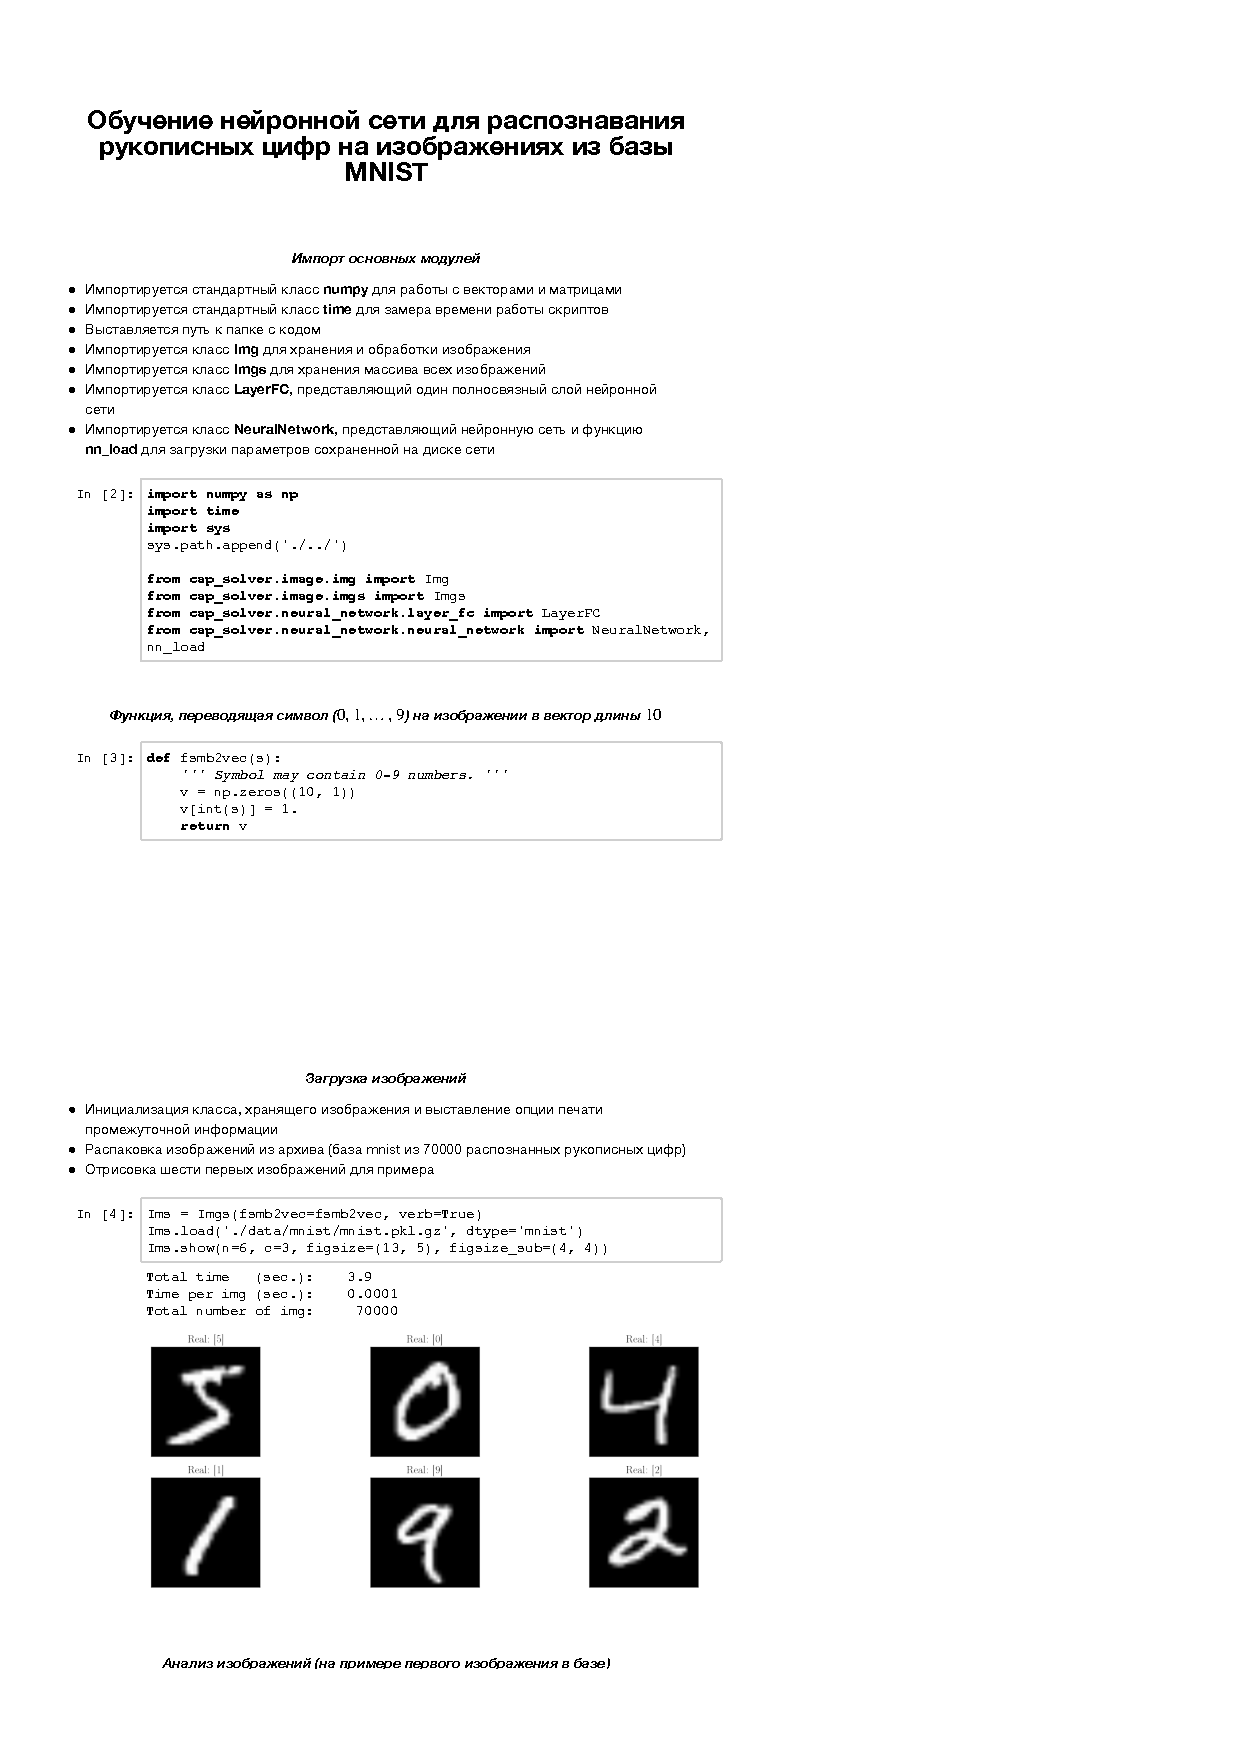
\includepdf[pages={1-7}]{mnist_recognition.pdf}

%=======================================================================
%\newpage
%\section*{ПРИЛОЖЕНИЕ В. Результаты обучения на примере реальной CAPTCHA} \label{app:captcha}
%\addcontentsline{toc}{section}{ПРИЛОЖЕНИЕ В. Результаты обучения на примере реальной CAPTCHA}

\end{document}